\newcommand{\FeynmanDiagramStau}{
\begin{figure}[!hbt]
\centering
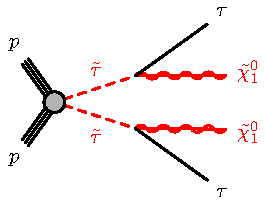
\includegraphics[width=0.7\textwidth]{Analysis/Feynman/staustau-tautauN1N1.pdf}
\caption{Diagram of the decay topology of the signal model considered in this work. A pair production of charged staus and subsequent decay into two-tau final state.}
\label{fig:feynman_direct_stau}
\end{figure}
}

\newcommand{\ABCDschematics}{
\begin{figure}[!hbt]
%\begin{wrapfigure}{R}{.5\textwidth}
	\begin{center}
		\subbottom[]{
			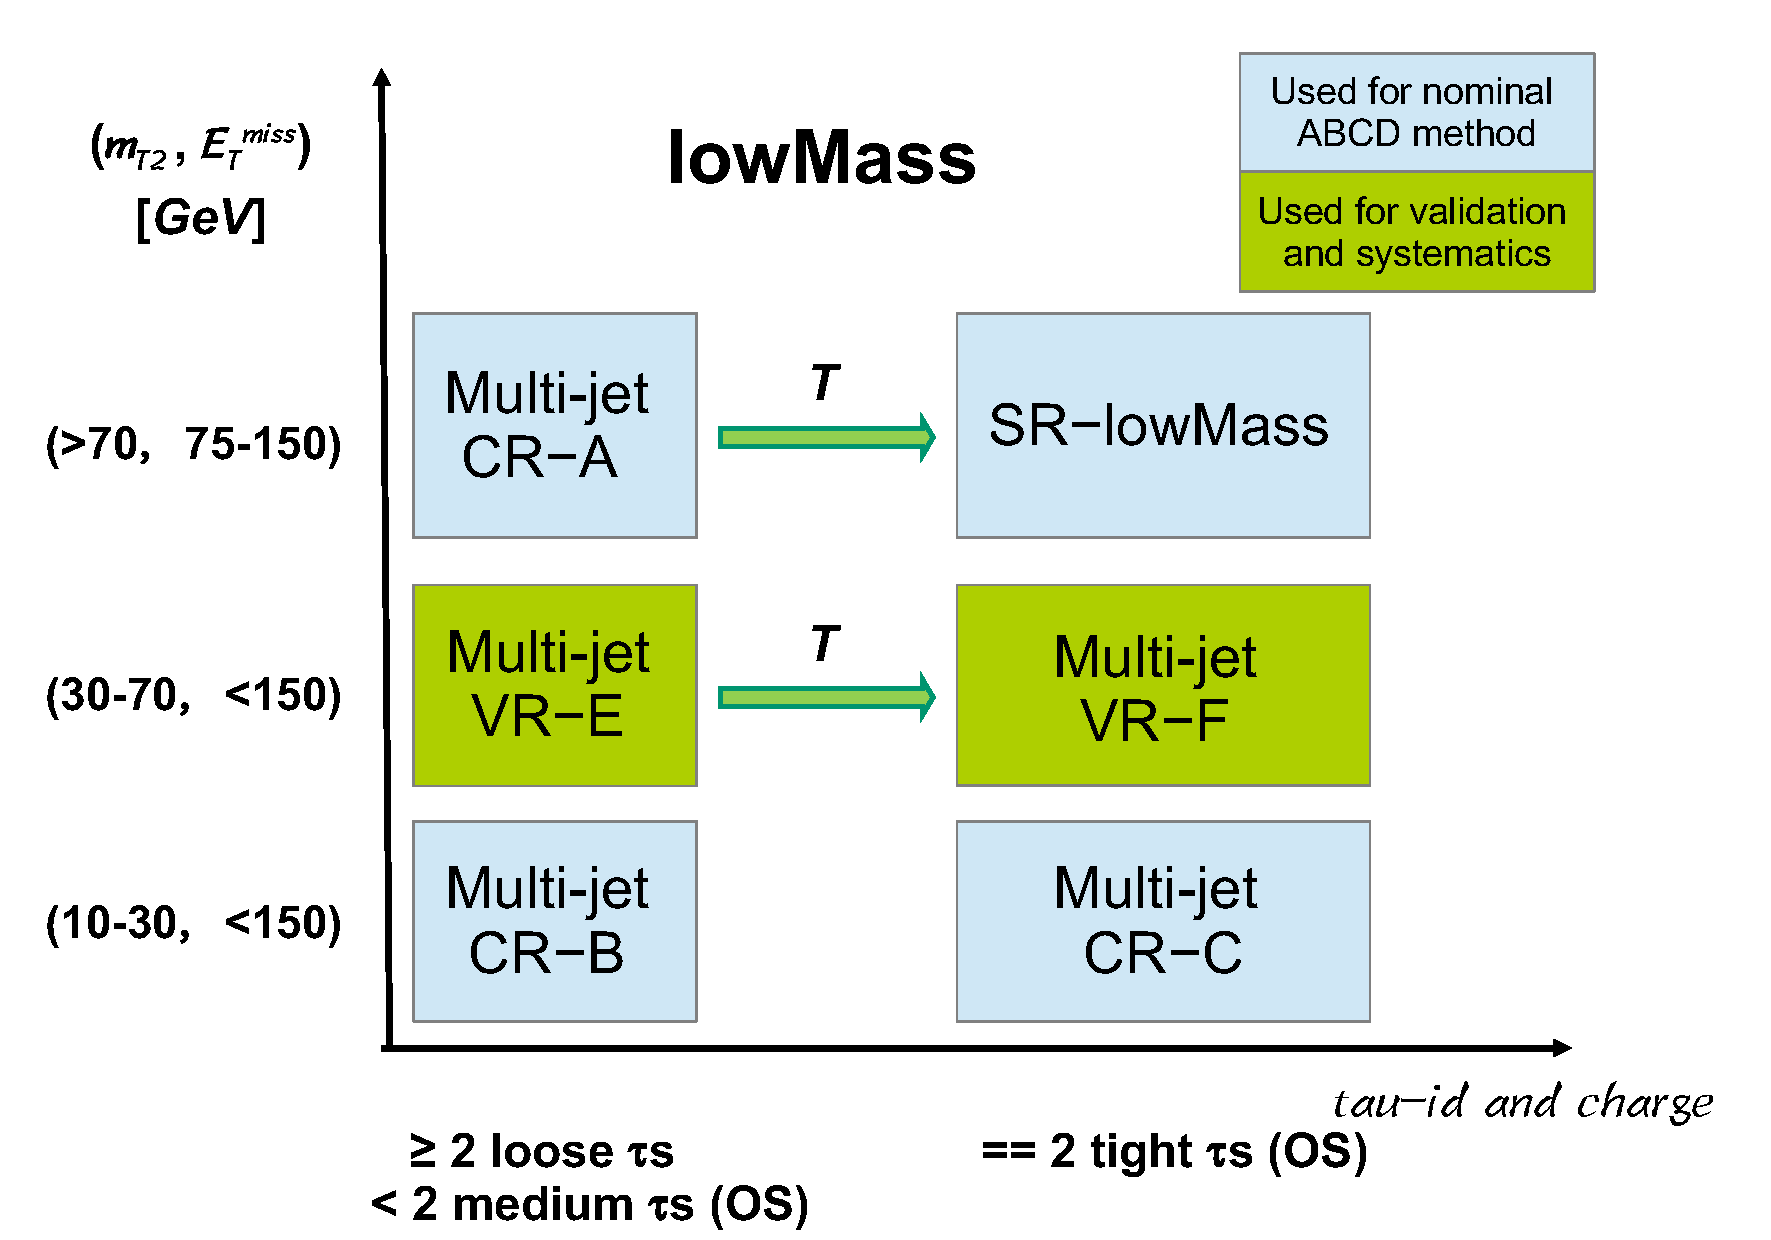
\includegraphics[width=0.49\textwidth]{Analysis/ABCD/ABCD_SR}}
		 \subbottom[]{
			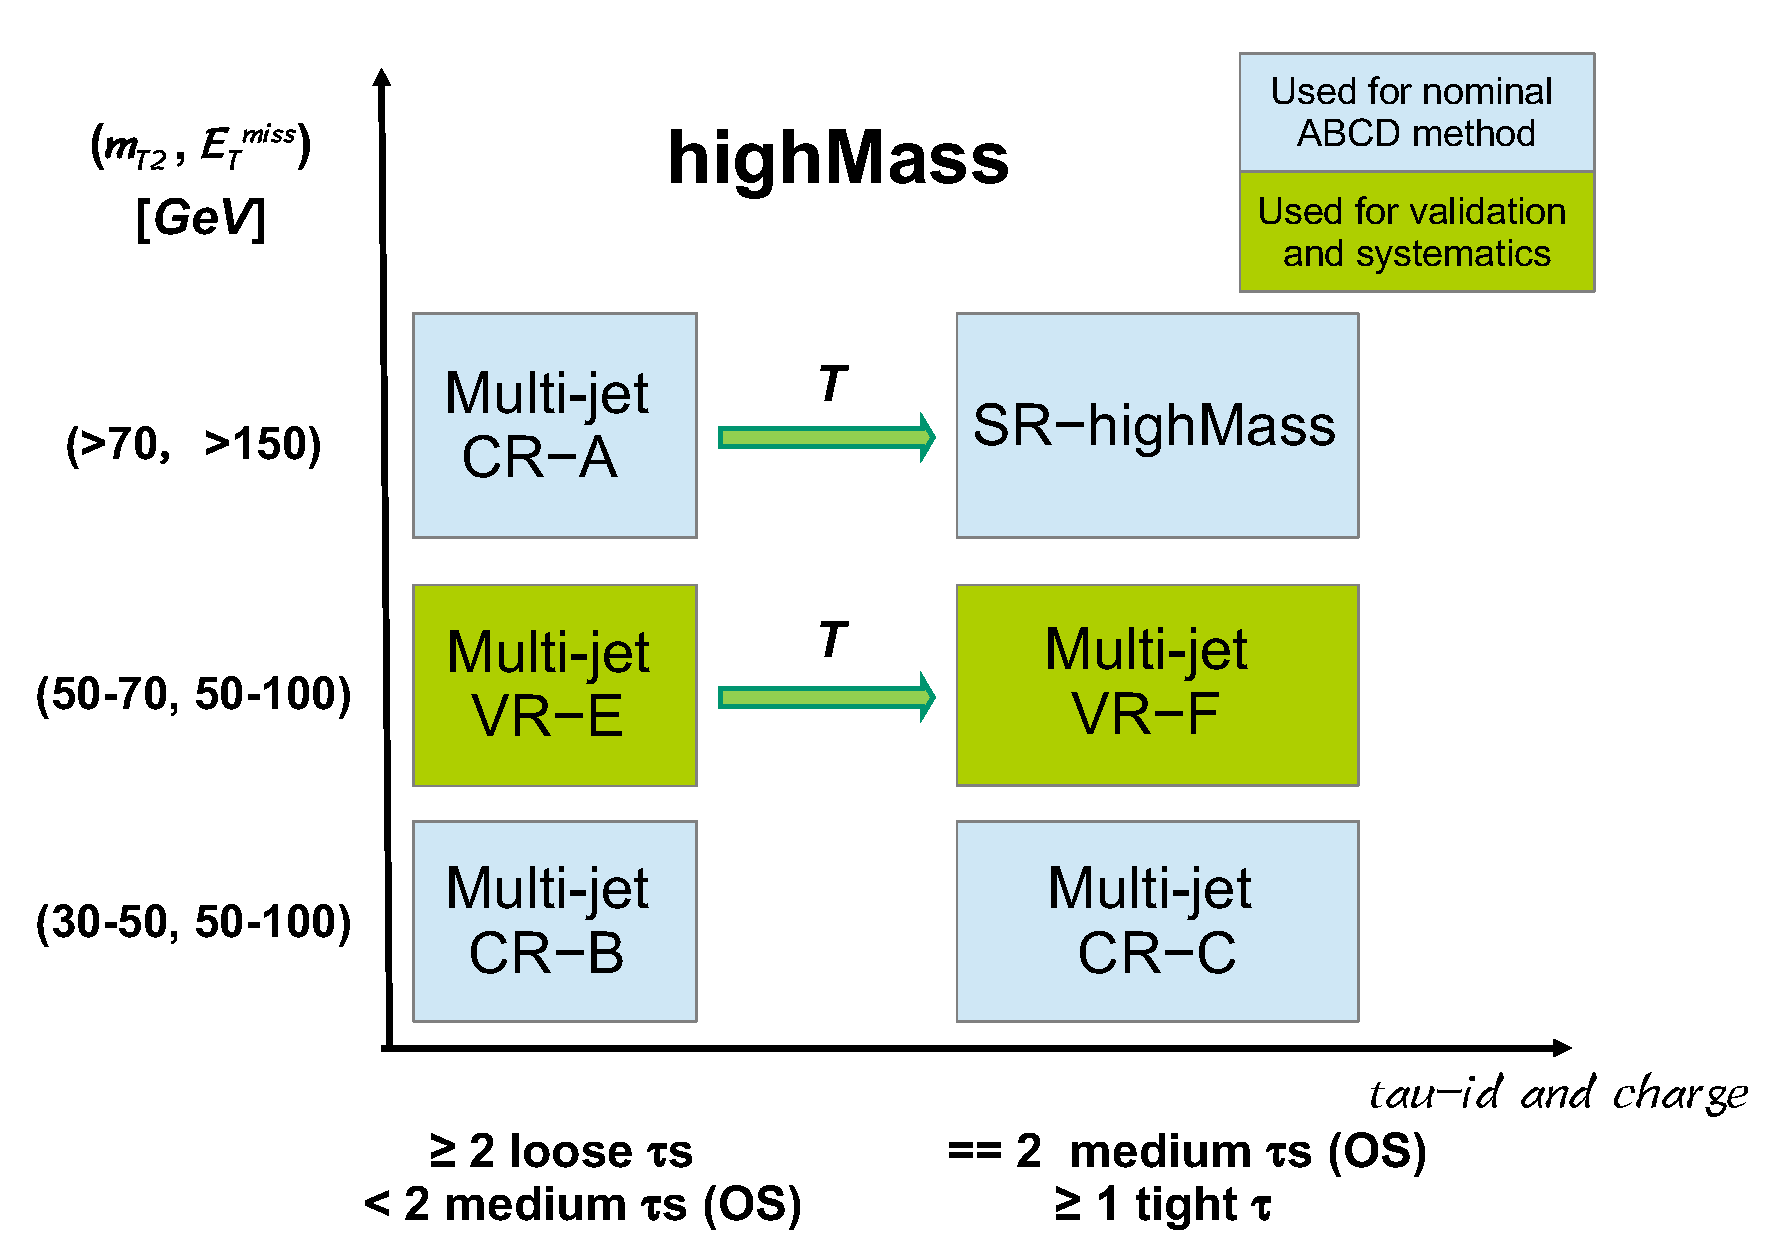
\includegraphics[width=0.49\textwidth]{Analysis/ABCD/ABCD_SR2}}
	\end{center}
\setlength{\belowcaptionskip}{-20pt}
\caption{Illustration of the ABCD method for the multi-jet background determination for (a) Low-mass and (b) High-mass \acp{SR}. \acp{CR} A, B, C, \ac{SR} D, and \acp{VR} E, F are described in the text and are drawn as blue and green boxes, respectively. 
%Regions E and F are \acp{VR} used to validate the ABCD method and to estimate the systematic uncertainty.
Transfer factor T used in the ABCD method is the ratio of number of multi-jet events in the regions C and B.}
\label{fig:ABCD_schematics}
\end{figure}
%\end{wrapfigure}
}

\newcommand{\SRyields}{
\begin{figure}[!hbt]
\begin{center}
\subbottom[]{
	\includegraphics[width=0.49\textwidth]{Analysis/SRL/mT21.pdf}}
	\subbottom[]{
	\includegraphics[width=0.49\textwidth]{Analysis/SRH/mT21.pdf}}
\end{center}
\caption{Post-fit $m_{T2}$ distribution for Low-mass \ac{SR} (left) and High-mass \ac{SR} (right). The stacked histograms show the expected \ac{SM} background. Contribution from \Wjets\ and multijet background events are scaled with the corresponding normalization factors derived from the background-only fit. The \ac{SUSY} signal point distributions are shown, for reference, as dashed lines.}
\label{fig:mT2_SR_yields}
\end{figure}
}

\newcommand{\exclusionstaustau}{
\begin{figure}[!hbt]
\centering
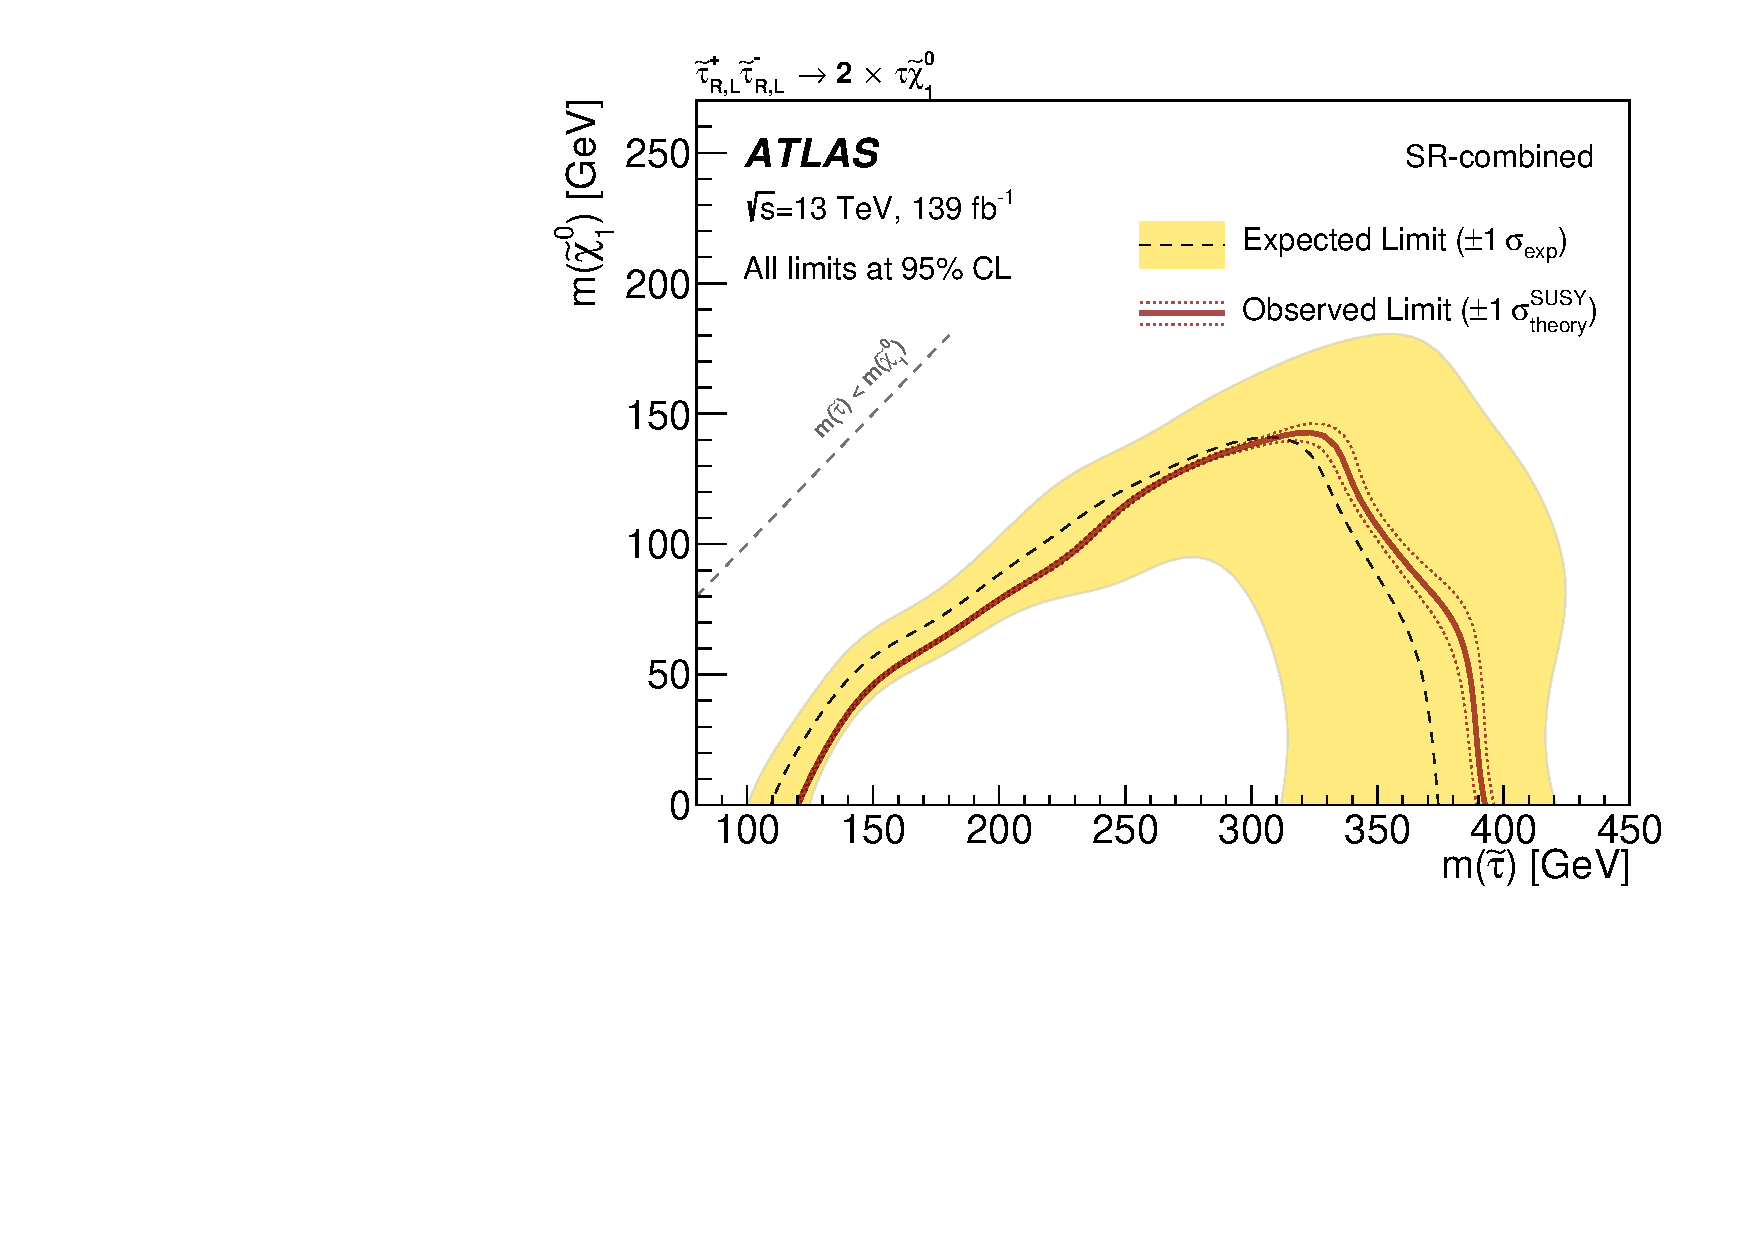
\includegraphics[width=\textwidth]{Analysis/Limits/limit_DS_combine_EXP_staustau.pdf}
\caption{95\% \ac{CL} exclusion limits for simplified models with direct \stau\ pair production in the combined High-mass and Low-mass \acp{SR}.}
\label{fig:exclusion_staustau}
\end{figure}
}

\newcommand{\exclusionstauLstauR}{
\begin{figure}[!hbt]
\begin{center}
\subbottom[]{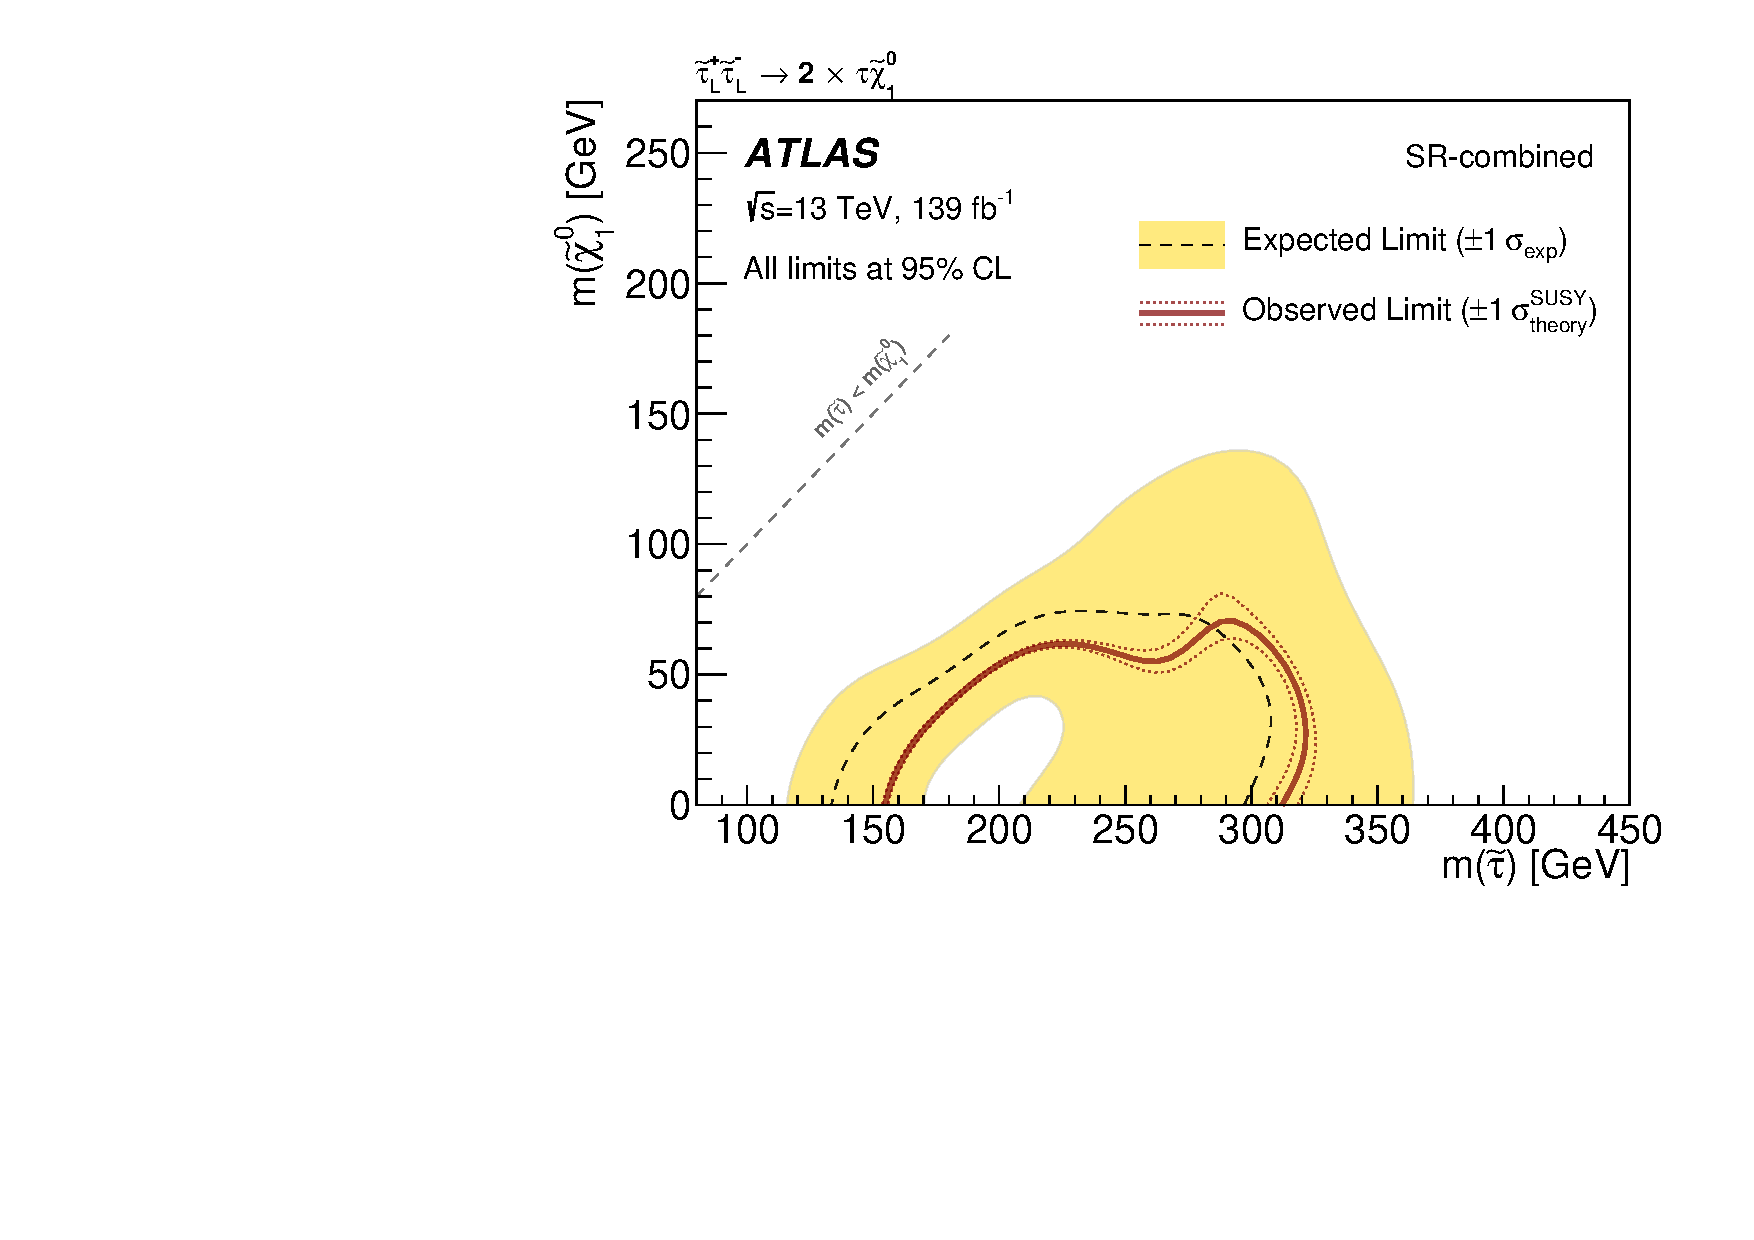
\includegraphics[width=0.7\textwidth]{Analysis/Limits/limit_DS_combine_EXP_stauL.pdf}}
\subbottom[]{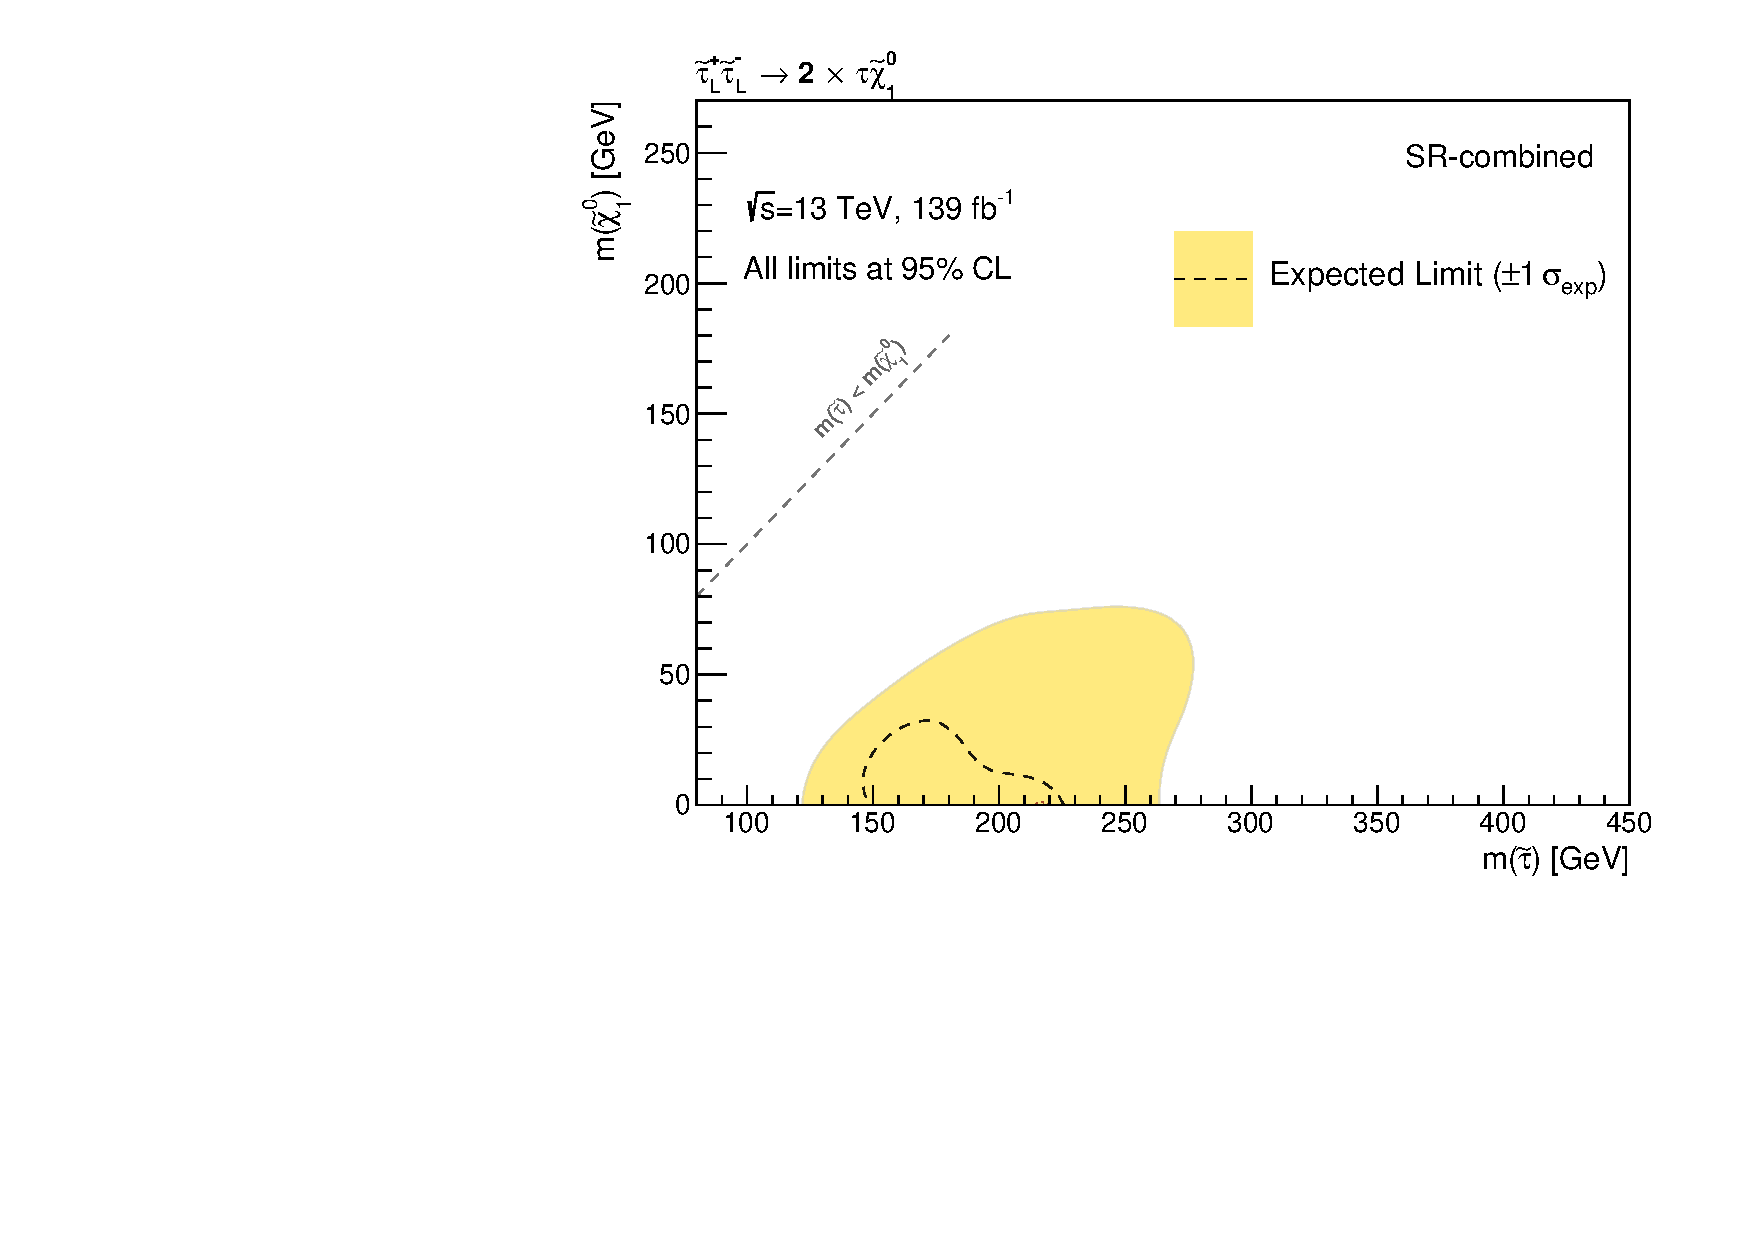
\includegraphics[width=0.7\textwidth]{Analysis/Limits/limit_DS_combine_EXP_stauR.pdf}}
\end{center}
\caption{95\% \ac{CL} exclusion limits for simplified models with direct (a) \stauL\stauL\ and (b) \stauR\stauR\ pair production in the combined High-mass and Low-mass \acp{SR}.}
\label{fig:exclusion_stauLstauR}
\end{figure}
}

\newcommand{\singleTauTrigTurnOn}{
\begin{figure}[!hbt]
\begin{center}
\subbottom[]{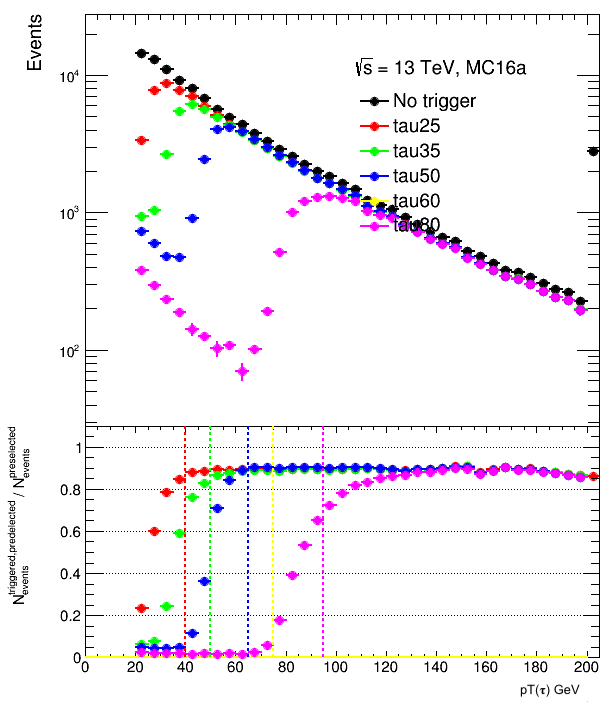
\includegraphics[width=0.33\textwidth]{Analysis/Trigger/TurnOn/WCR_tau1pt_mc16a.png}}
\subbottom[]{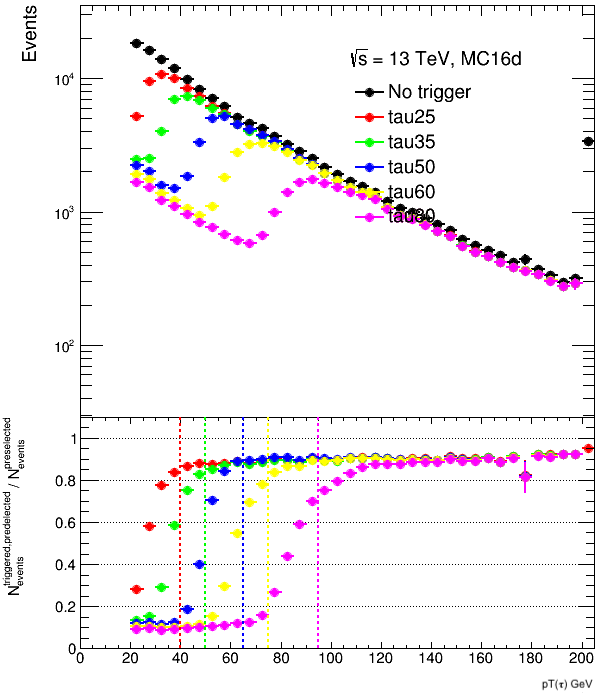
\includegraphics[width=0.33\textwidth]{Analysis/Trigger/TurnOn/WCR_tau1pt_mc16d.png}}
\subbottom[]{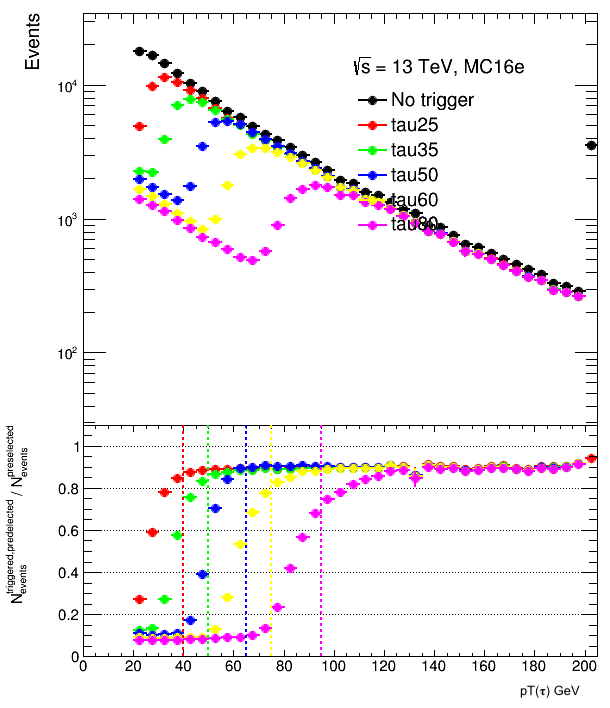
\includegraphics[width=0.33\textwidth]{Analysis/Trigger/TurnOn/WCR_tau1pt_mc16e.png}}
\end{center}
\caption{Turn-on curves of single tau triggers on \ac{SM} background samples, simulated in \ac{MC} for (a) 2015-2016, (b) 2017, and (c) 2018 data. Dashed line represents estimated turn-on thresholds.}
\label{fig:tau_single_leg_turnon}
\end{figure}
}

\newcommand{\metTrigTurnOn}{
\begin{figure}[!hbt]
\begin{center}
\subbottom[]{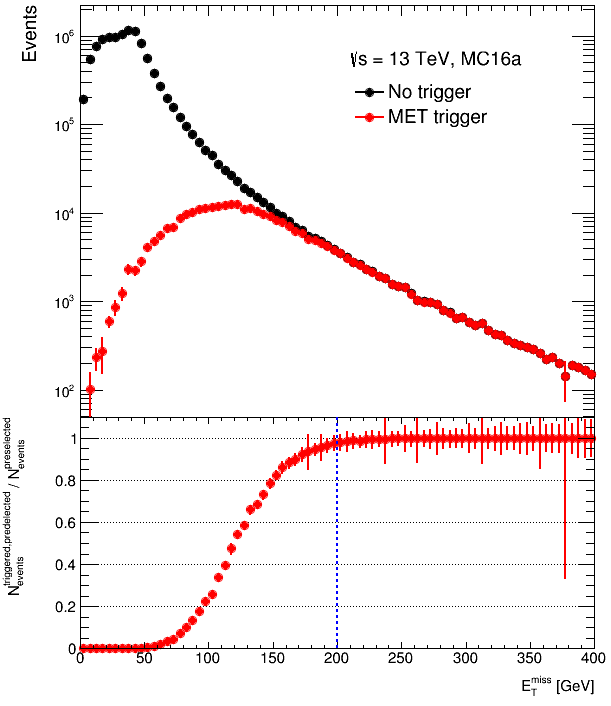
\includegraphics[width=0.33\textwidth]{Analysis/Trigger/TurnOn/MetTST_met_mc16a.png}}
\subbottom[]{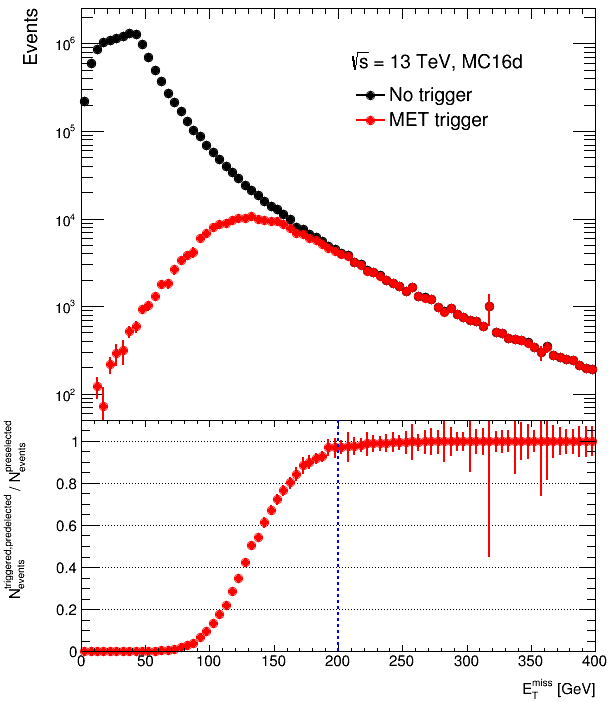
\includegraphics[width=0.33\textwidth]{Analysis/Trigger/TurnOn/MetTST_met_mc16d.png}}
\subbottom[]{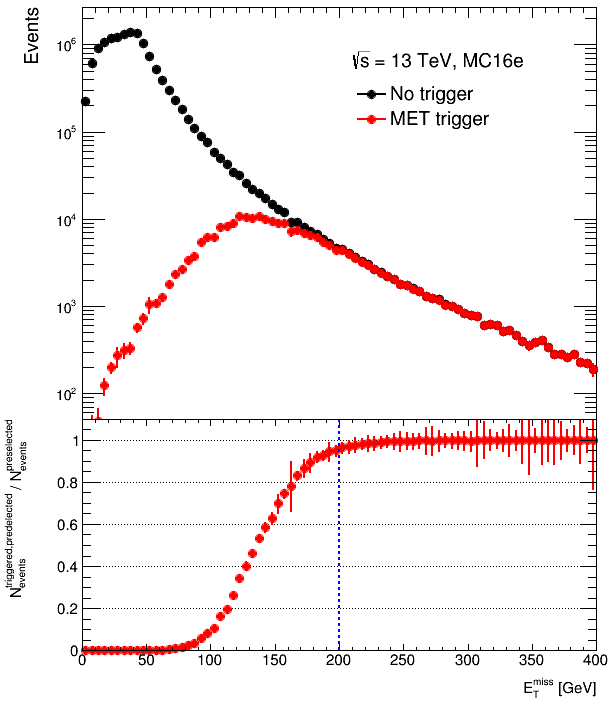
\includegraphics[width=0.33\textwidth]{Analysis/Trigger/TurnOn/MetTST_met_mc16e.png}}
\end{center}
\caption{Turn-on curves of 50\gev\ online threshold \met\ trigger on \ac{SM} background samples, simulated in \ac{MC} for (a) 2015-2016, (b) 2017, and (c) 2018 data. Dashed line represents estimated turn-on thresholds.}
%\met\ trigger turn on curves}
\label{fig:mettrig_turnon}
\end{figure}
}

\newcommand{\metTrigKine}{
\begin{figure}[!hbt]
\begin{center}
%\subbottom[$p_T(\tau)$]{
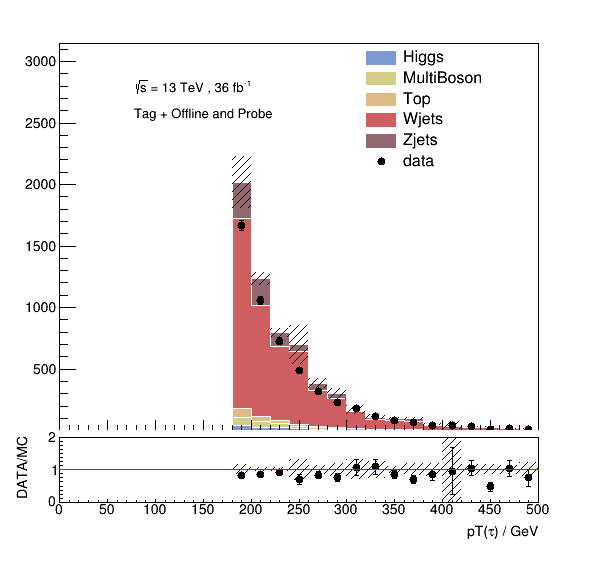
\includegraphics[width=0.45\textwidth]{Analysis/Trigger/MET/kine_pt0_xe50.png}
%}
%\subbottom[\met]{
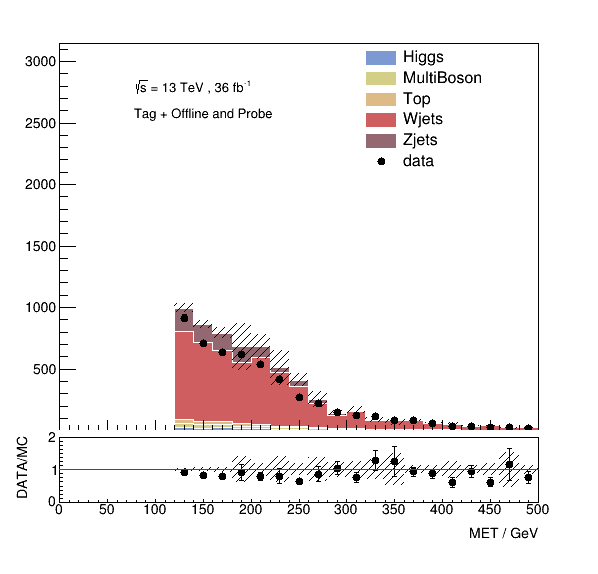
\includegraphics[width=0.45\textwidth]{Analysis/Trigger/MET/kine_met_xe50.png}
%}
\end{center}
\caption{Kinematic distributions of \ltau\ \pt\ (left) and \met\ (right) for Tag and Probe method selection. \ac{SM} background are shown by the stacked histograms while data is represented by black markers. Statistical uncertainties are shown by shaded area.}
\label{fig:TnP_kine}
\end{figure}
}

\newcommand{\metTrigEff}{
\begin{figure}[!hbt]
\begin{center}
%\subbottom[]{
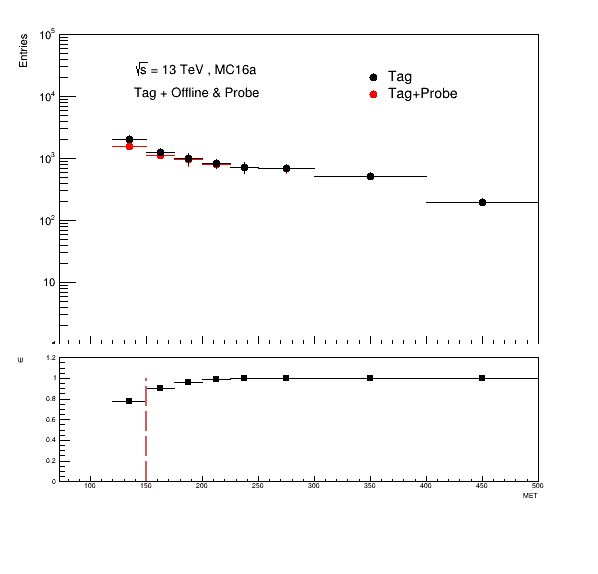
\includegraphics[width=0.45\textwidth]{Analysis/Trigger/MET/Efficiency_SUSY3_MC16a_xe50.png}
%}
%\subbottom[]{
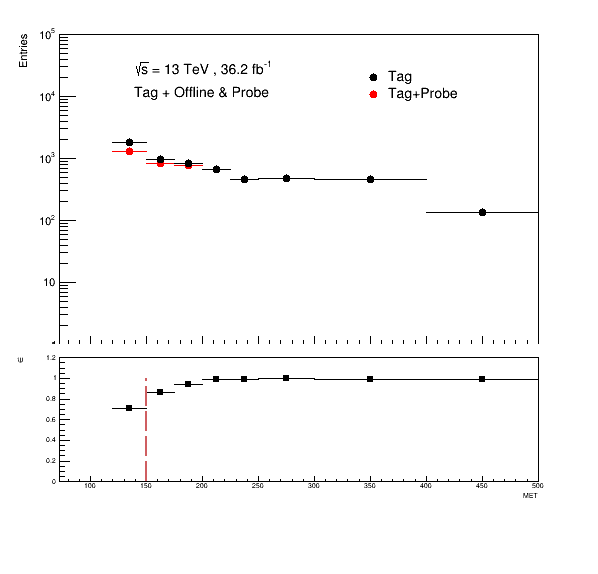
\includegraphics[width=0.45\textwidth]{Analysis/Trigger/MET/Efficiency_DATA16_xe50.png}
%}
%\subbottom[]{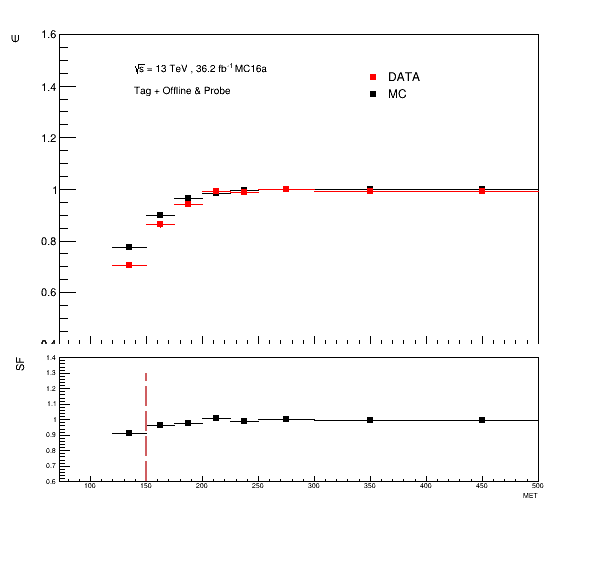
\includegraphics[width=0.45\textwidth]{Analysis/Trigger/MET/SF_xe50.png}}
\end{center}
\caption{\met\ distributions using Tag (black) and Probe (red) method for 50 \gev\ threshold \met\ trigger for a combined set of \ac{MC} simulated \ac{SM} backgrounds (left) and 36.2 \infb\ of data collected in 2016 (right). Bottom plot show corresponding efficiencies. }
%\setlength{\abovecaptionskip}{-50pt}
\label{fig:TnP_eff}
\end{figure}
}

\newcommand{\metTrigSF}{
%\begin{wrapfigure}{R}{.5\textwidth}
\begin{figure}[!hbt]
\centering
%\begin{center}
%\subbottom[]{
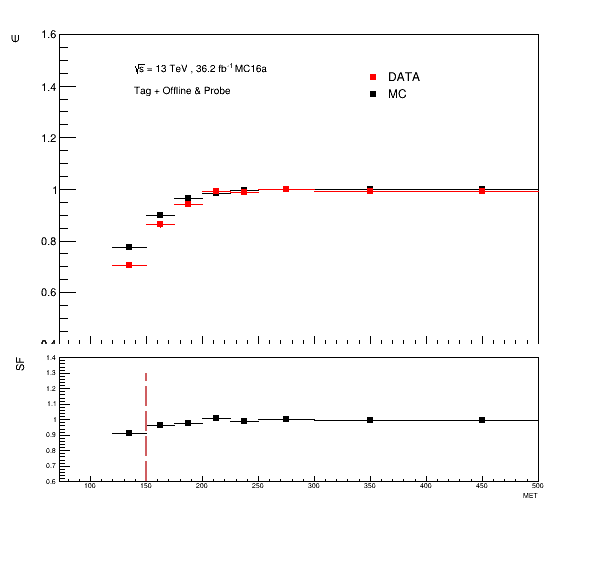
\includegraphics[width=0.6\textwidth]{Analysis/Trigger/MET/SF_xe50.png}
%}
%\end{center}
\caption{Efficiency plot of 50 \gev\ threshold \met\ trigger for combined \ac{MC} \ac{SM} backgrounds (black) and collected data (red). \ac{SF} values as a function of \met\ are shown in the bottom plot. Online \met\ thresholds shown on as vertical red dashed line.}
\label{fig:TnP_SF}
\end{figure}
%\end{wrapfigure}
}

\newcommand{\ditauClosureTest}{
\begin{figure}[!hbt]
\begin{center}
\subbottom[tau80\_tau60]{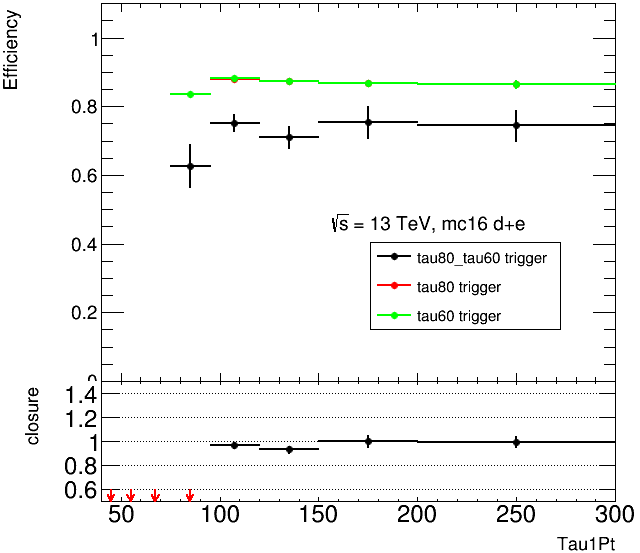
\includegraphics[width=0.33\textwidth]{Analysis/Trigger/Closure/tau80_tau60_closure.png}}
\subbottom[tau80\_tau50]{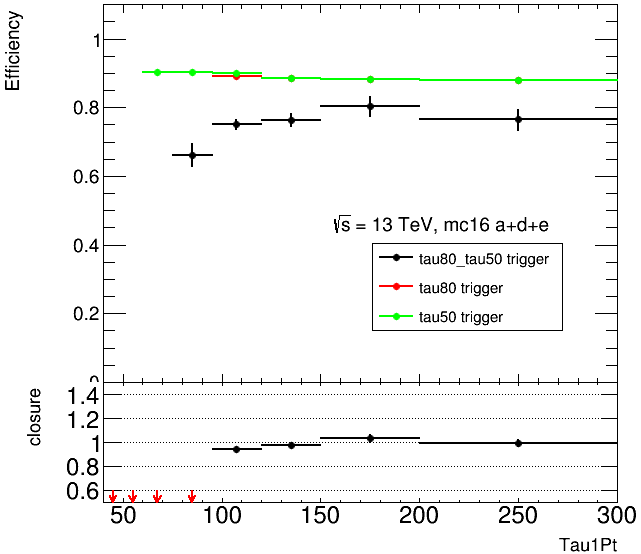
\includegraphics[width=0.33\textwidth]{Analysis/Trigger/Closure/tau80_tau50_closure.png}}
\subbottom[tau35\_tau25]{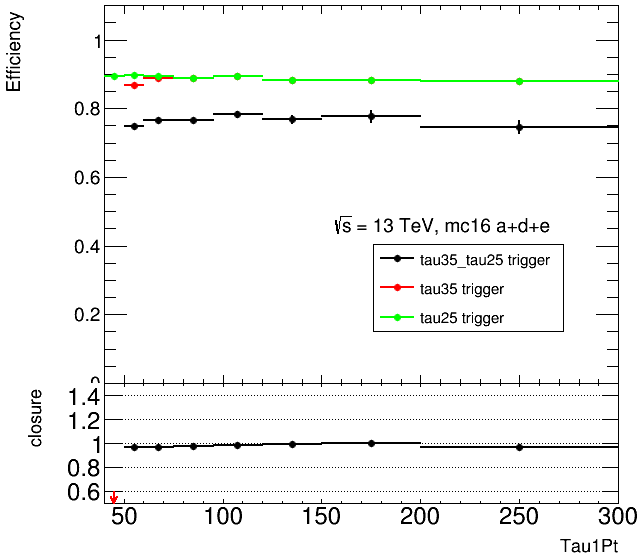
\includegraphics[width=0.33\textwidth]{Analysis/Trigger/Closure/tau35_tau25_closure.png}}
\end{center}
\setlength{\belowcaptionskip}{-20pt}
\caption{Closure test for di-tau trigger efficiencies using for tau trigger legs of the asymmetric di-tau and di-tau+\met\ triggers.
 Single tau trigger efficiencies are shown in green and red for each leg of the di-tau trigger. Combined trigger efficiency is shown in black. }
\label{fig:tau_single_leg_closure}
\end{figure}
}

\chapter{Search for direct stau production}
\label{ch:analysis}
%\epigraph{\emph{Life is not a game of luck. If you wanna win, work hard}}{Nai Sora - No Game No Life}
%\epigraph{\emph{I am just a dreamer, but you are just a dream}}{Niel Young}
\epigraph{\emph{Go closer hold the land feel partly no more than grains of sand. 
						We stand to lose all time a thousand answers by in our hand. 
						Next to your deeper fears we stand.
						Surrounded by million years.}}{Yes}

This chapter presents the analysis strategy, optimization and results of the search for direct production of supersymmetric partner of the \ltau\ in all-hadronic final state, using data collected during the Run-2 data-taking period, totalling in 139 \infb\ of $pp$ collisions at a centre-of-mass energy \com $=13$ \tev.
 In Section~\ref{sec:stratintro} an introduction to the analysis, including the motivation of the search, the signal process considered and the adopted analysis strategy is presented; 
 Sections~\ref{sec:susysig} and ~\ref{sec:smsamples} describe the \ac{SUSY} and \ac{SM} \ac{MC} generated samples used for this analysis.
 The reconstruction of the particle objects used, in both data and \ac{MC}, is described in Section~\ref{sec:objdef}. 
The study of the combined tau triggers \acp{SF} and efficiencies used in the selection of relevant events in the analysis \acp{SR} was performed by the author and is presented in Section~\ref{sec:anatrig}.
Section~\ref{sec:evtsel} describes the \ac{SR} optimisation performed by the author to isolate the signal events from the \ac{SM} background, and the background estimation methods performed for the most significant background processes. 
A major contribution of the author's work has been in the estimation of the systematic uncertainties which affect this analysis, described in Section~\ref{sec:syst_unc}. Finally, a description of the statistical analysis used, together with the corresponding results. and interpretation are given in Sections~\ref{sec:stat_ana}, ~\ref{sec:results}, and ~\ref{sec:interpretation}, respectively. 


	\section{Introduction and Strategy}
	\label{sec:stratintro}
	As already discussed in Chapter ~\ref{ch:theory}, the \ac{SUSY} extension to the \ac{SM} is an appealing proposed theory to solve the fine-tuning problem. If R-parity~\cite{JUNGMAN1996195} is conserved, \ac{SUSY} particles are produced in pairs at the \ac{LHC}, with the \ac{LSP} being stable and weakly interacting and thus a strong candidate for dark-matter.
	In the \ac{MSSM} the coloured sparticles (squarks and gluinos) have a high mass, and the weakinos instead have a low mass.
	 In this case, the first signs of \ac{SUSY} at the \ac{LHC} can be spotted in events with high lepton multiplicity and low jet activity, such as the decay of the electro-weakinos (charginos \chinopm\ and neutralinos \nino) and the sleptons (\slepton\ and \snu).
	 
	
	For this analysis only the direct production of \stau\ from $pp$ interaction at the \ac{LHC} is considered, as shown by Figure ~\ref{fig:feynman_direct_stau}. The considered final states signature is composed of two hadronically decaying \ltau s with low jet activity and large missing transverse energy (\met), originating from the neutralinos and neutrinos.	
	The signal considered in this work is generated using a simplified model, where the scalar superpartner of the left-handed $\tau$-lepton (\stauL), right-handed $\tau$-lepton  (\stauR), and the lightest neutralino (\ninoone) are the only \ac{SUSY} particles considered. 
	In this model the \ninoone\ is considered to be the \ac{LSP} while the \stauL\ and \stauR\ are assumed to be mass-degenerate and have 100\% branching fraction into \ninoone\ and $\tau$-lepton.
	 
%	 In this the only direct production of \stau\ from $pp$ interaction at the \ac{LHC} is considered, as shown by Figure ~\ref{fig:feynman_direct_stau}. The main signatures of the studied final states are two hadronically decaying taus with low jet activity and large missing transverse energy (\met) from the neutralinos and neutrinos. 
	
	\FeynmanDiagramStau 
		 
	Final states with hadronic $\tau$-leptons can be experimentally challenging due to the difficulty in the reconstruction and identification of these particles in the \ac{ATLAS} detector. The methods and challenges of \ltau\ reconstruction and identification will be discussed in more detail later in the Chapter.
	Nonetheless, they are of particular interest in \ac{SUSY} searches since light sleptons could play an important r$\mathrm{\hat{o}}$le in the co-annihilation of neutralinos in the early universe, and models with light scalar taus are consistent with dark-matter searches~\cite{Albornoz_V_squez_2011}.  
	 
	\section{SUSY signal}
	\label{sec:susysig}
	%The simulated $\tau\rightarrow\tau\nino$ signal process studied 
	The masses of all charginos and neutralinos, apart from the \ninoone, are set to 2.5 \tev\ so that they are decoupled from the phenomenology under study. 
	This leaves only a single kinematically allowed decay: $\stau^{\pm}\rightarrow\ninoone\tau^{\pm}$.  
	The masses of the other sleptons are also decoupled and not included in the production. 
	The masses of the left-hand and right-hand \stau\ are degenerate, and vary between 100-400 \gev. The mass of the bino-like \ninoone is varied between the range of 0-200 \gev.
	Most results that will be shown will use reference points with \stau\ masses of 120 \gev, 280 \gev, and a \ninoone\ mass of 1 \gev\ to illustrate typical features of the \ac{SUSY} models that this analysis is sensitive to.
	
	The signal samples for this work have been generated using \textsc{MadGraph5\_aMC@NLO 2.6.2}~\cite{madgraph} interfaced with \textsc{Pythia 8.186} with the \textsc{A14} tune~\cite{ATL-PHYS-PUB-2014-021} for the \ac{PS} modelling, hadronisation, and underlying event. The \textsc{NNPDF2.3LO} \ac{PDF}~\cite{BALL2013244} has been used for the \ac{ME} calculation, and includes the emission of up to two additional partons. The nominal cross section and its uncertainty has been taken from an envelope of cross section predictions using different \ac{PDF} sets and factorization and renormalization scales, as described in References \cite{cite-1,Beenakker:1999xh,Bozzi_2007,Fuks_2014,Fiaschi_2018}.
	The theoretical cross section used at \ac{NLO + NLL} was 140 (50) fb with \stauL\stauL (\stauR\stauR) of 120 \gev, and 5.8 (2.2) fb with \stauL\stauL (\stauR\stauR) of 280 \gev.~\cite{PhysRevD.101.032009}

	\section{SM samples}
	\label{sec:smsamples}
	In order for the analysis to robustly target the desired signal, the accurate modelling of background processes is fundamental. For this type of analysis there is a wide variety of \ac{SM} processes whose cross sections are significantly larger than of the \ac{SUSY} signal process of interest. These \ac{SM} processes, thus, constitute the background of the analysis.  
	The definition of a \ac{SR} must take into account the kinematic properties and multiplicities of the final state particles of the target signal and background processes to achieve the highest possible discrimination between the two. The defined signal region will thus be most sensitive to the target signal events.
	In order to construct a high sensitivity \ac{SR}, background processes need to be accurately simulated in \ac{MC} events.  
	%is strictly related to the sensitivity of reached by the analysis and needs to accurately account for the kinematic properties of both the target signal and background processes.  
	The backgrounds that significantly contribute to the search of direct \stau\ production in a di-$\tau+$\met\ final state scenario, with their relative \ac{MC} samples, are discussed below. 
		%The \ac{SM} backgrounds included in this analysis, which are simulated with \ac{MC}, are \Zjets, including off-shell production of the Z-boson, multi-boson (VV and VVVV), \ttbar, \ttV, \ttX, and single top production.
	\begin{description}
	\item[W boson production in association with jets:] the production of $W$ boson with jets is a relevant background for our search, due to the $W\rightarrow\ell\nu$ ($\ell=e,\mu,\tau$) decay, with a \ac{BR} of $\sim32\%$). The production of \Wjets\ events where at least one jet is misidentified as a tau is thus an important background to this search.
	\item[Z boson production in association with jets:] the production of $Z$ boson in association with jets is one of the main \ac{SM} backgrounds of our analysis. The $Z$ boson will decay via $Z\rightarrow\ell\ell$ ($\ell=e,\mu,\tau$), with a \ac{BR} of $\sim10\%$, thus contributing significantly to the \ac{SM} background producing final states with two real taus.
	\item[Multi boson production:] the production of di- or multi- boson ($VV$, $VVV$ where $V=W,Z$), are also a significant source of background events containing real tau leptons. The real taus in the multi boson production come from the $WW$ and $ZZ$ processes that decay into a $\tau\tau\nu\nu$ final state with \ac{BR} of $\sim10\%$ and $\sim2\%$, respectively.~\cite{PDG}
	\item[Top single and pair production:] single top, \ttbar\ production in association with jets, or top with an additional $W$ or $Z$ boson are collectively referred to as 'top' background.  The different decays from the single top process are generally separated into the different channel-types (\textit{s}-channel,\textit{t}-channel). All these background processes contribute towards the amount of irreducible background present in this analysis. The dominant top-quark decay is $t\rightarrow W$ with \ac{BR} of $\sim99\%$. This can in turn yield 0-lepton, 1-lepton and 2-lepton final states with $45.7\%$, $43.8\%$ and $10.5\%$ \ac{BR}, respectively. The irreducible background contribution will therefore come from the 2-lepton final state, and from the other two channels when there is at least one mis-identified jet in the event.
	\item[Higgs boson production:] there is a small contribution of from higgs boson events produced by gluon-gluon fusion and vector boson fusion. These events only contribute in small part the total irreducible background, but have still been included in this analysis. 
	\item[Multi-jet:] the multi jet production is the process with the highest cross section among the ones mentioned thus far. Despite the low probability of mis-identifying two jets as real taus, because of the large cross section of this process the background will generate a non-negligible contribution. There is also a significant contribution arising from heavy-flavour multi-jet events containing a real tau lepton from the heavy-flavour quark decay as part of the total multi-jet estimate.
	\end{description}
	
	\section{Object Definition}
	\label{sec:objdef}
	Reconstructed objects are required to pass a "loose" selection to be categorised as \textit{baseline} objects. 
	This indicates that these objects have been reconstructed with enough precision that they can be used for further analysis. 
	These baseline objects need are used as inputs for the \ac{OR} procedure described below.
	The resulting objects are referred to as \textit{signal} objects after  they pass some additional selection criteria.
	The baseline and signal objects are defined as:
	
	\begin{description}
	\item[Taus] only the visible part of the $\tau$ decay is reconstructed for the candidates candidates that are associated with a primary vertex. Taus not associated to a primary vertex are not considered.  
	An energy calibration derived independently of the jet energy scale is applied to the reconstructed $\tau$ objects.
	$\tau$ candidates with \pt\ $<$ 20 \gev\ and $|\eta|>2.5$, or in the region of 1.37 $<|\eta|<$ 1.52 are rejected. A total track charge of $\pm$ 1 is required with the presence of 1 or 3 associated tracks.  
	A \ac{BDT} discriminant is used to reject jets that do not originate from a hadronically decaying tau leptons with a \textit{Medium} working point for the signal taus and a minimum value of 0.01 for the baseline tau (see paragraphs below for more detailed description of reconstruction and identification algorithms with corresponding working points).
	\item[Electrons] Electrons must pass the Tight (loose) likelihood identification criterion to be signal (baseline) candidates. Signal electrons are required to satisfy an isolation criteria to reduce the number of jets mis-identified as charged leptons.\footnote{The scalar sum of \pt\ of tracks inside the variable-size cone around the lepton must be less that 15\% of the lepton \pt. The track isolation cone size is given by $\Delta R\, =\,10\, \mathrm{GeV}\, /\, p_T$ and must be less than 0.2.}  For electrons with \pt$>200$ \gev\ this requirement does not apply and instead an isolation requirement using a fixed size cone ($\Delta R\,<\,0.2 $) is used. Electrons must have \pt\ $>17$ \gev\ and $|\eta|\,<\,2.47$.
	%Electron candidates are reconstructed by matching clusters in the \ac{EM} calorimeter  with charged particle tracks in the \ac{ID}.
	\item[Muons] Muon candidates must pass the \textit{Medium} selection criteria, defined in Reference ~\cite{ATLASMuonRecoRun2}, and must satisfy \pt $>\,14$ \gev\ and $|\eta|\,<$ 2.7. A loose fix cut working point is applied to select the isolated signal muons. 
	\item[Jets and b-tagging] Reconstructed jets are calibrated using a \ac{JES} derived from simulation and in situ corrections based on 13 \tev\ data ~\cite{ATL-PHYS-PUB-2015-015,ATLAS-CONF-2015-037}. Jets are required to have \pt\ $>\,20$ \gev\ and $|\eta|\,<$ 2.8. Events with at least one jet arising from non-collision sources or detector noise are removed ~\cite{ATLAS-CONF-2015-029}, resulting in negligible loss of efficiency. An additional \textit{Medium} working point requirement on the \ac{JVT} is made for jets with \pt\ $<$ 20 \gev\ in central  ($|\eta|\,<$ 2.5) region of the detector to avoid selecting jets from secondary $pp$ interactions.
	In \ac{ATLAS} reconstructed jets are identified as originating from the hadronisation of a $b$-quark ($b$-tagged) via the \textsc{MV2c10} algorithm~\cite{Aaboud_2018}. 
	\item[Missing transverse momentum] The missing transverse momentum observable (\met) is defined as the size of the vectorial sum \pt\ of all selected and calibrated physics objects in the event, with an extra term added to account for soft energy in the event that is not associated to any of the selected objects. This soft term is calculated from \ac{ID} tracks associated to the primary vertex to make it more resilient to pileup contamination~\cite{ATLASMet2015,ATLASMet2012}.
	\end{description}
	
	The reconstruction algorithms in \ac{ATLAS} run independently from each other. Thus, it may happen that the detector signatures stemming from one physical object are reconstructed as two or more different objects. 
	To resolve these ambiguities, a procedure is defined which looks for reconstructed objects that lie within a certain cone to decide which particle should be kept or removed. This procedure is commonly referred to as the Overlap Removal Procedure (\ac{OR}). 
	The fixed set of requirements which the different objects need to pass for the overlap removal procedure used for this analysis are shown in Table ~\ref{tab:analysis_OLR}.
	
	\begin{table}[!hbt]
	\centering
	\caption{Consecutive steps of the overlap removal procedure used in the direct stau analysis. All objects used in the \ac{OR} are baseline objects.}
	%\documentclass[10pt]{article}
%\usepackage[usenames]{color} %used for font color
%\usepackage{amssymb} %maths
%\usepackage{amsmath} %maths
%\usepackage[utf8]{inputenc} %useful to type directly diacritic characters
%\begin{document}
%\begin{table}[]
\begin{tabular}{cccc}
\hline 
Step & \begin{tabular}[c]{@{}c@{}}Object \\ removed\end{tabular} & \begin{tabular}[c]{@{}c@{}}Object \\ compared against\end{tabular} & Condition \\ \hline \hline
1. & electron & electron & shared track \\
2. & tau & electron & $\Delta R\,<\,0.2$ \\
3. & tau & muon & $\Delta R\,<\,0.2$ \\
4. & electron & muon & shared ID track \\
5. & jet & electron & $\Delta R\,<\,0.2$ \\
6. & electron & jet & $\Delta R\,<\,0.4$ \\
7. & jet & muon & \begin{tabular}[c]{@{}c@{}}N. tracks < 3 and \\ $\Delta R\,<\,0.2$\end{tabular} \\
8. & muon & jet & $\Delta R\,<\,0.4$ \\
9. & jet & tau & $\Delta R\,<\,0.2$ \\ \hline 
\end{tabular}
%\end{table}
%
%\end{document}	
	\label{tab:analysis_OLR}
	\end{table}
	
	The analysis described in this chapter is particularly susceptible to the reconstruction and identification efficiency of hadronically decaying \ltau s, in the \ac{ATLAS} detector. 
	The method and performance of the \htau\ reconstruction and identification algorithms are thus summarised in the following paragraphs. 	
	
	\subsection*{Hadronic tau Reconstruction}
	The \htau\ reconstruction algorithm uses jets formed using the anti-$k_t$ algorithm with distance parameter $R=0.4$ and clusters of calorimeter cells, calibrated using a \ac{LC} as input seeds  for the reconstruction algorithm. These seed jests must also satisfy a \pt\ $>$ 10 \gev and $|\eta|\,<$ 2.5 requirement. Tracks associated to the \htau\ candidate must also follow some criteria. They are required to be within a cone of $\Delta R\,<$ 0.2 around the \htau candidate direction and also satisfy the following criteria: \pt $>$ 1 \gev, at least two associated hits in the pixel detector (including \ac{IBL}), and at least seven hits total in the pixel and \ac{SCT} detector. More details on the requirements and methodology of \htau\ reconstruction can be found in reference ~\cite{ATL-PHYS-PUB-2015-045}.
	
	\begin{wrapfigure}{R}{.53\textwidth}
			  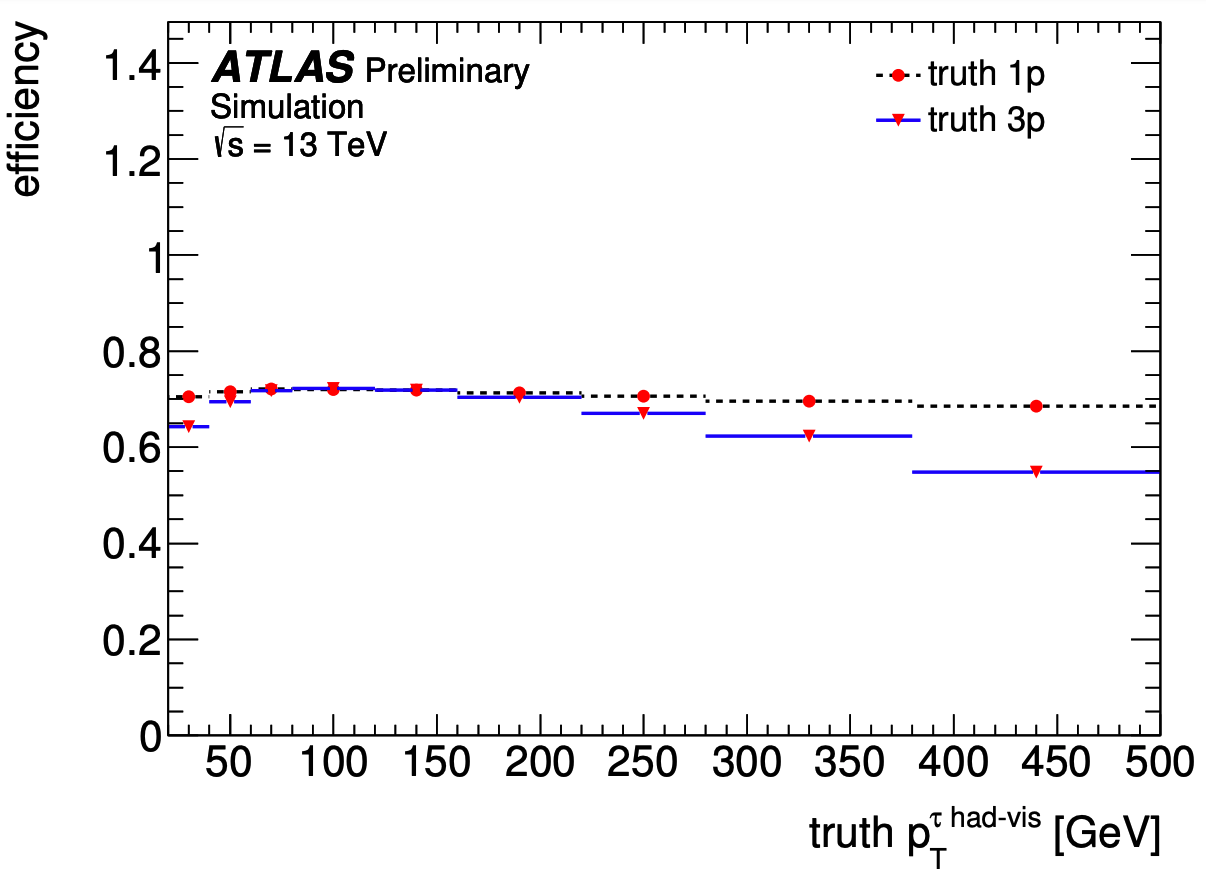
\includegraphics[width=0.5\textwidth]{FakeTau/tau_reco_eff_plt}
			  \caption{Efficiency for reconstructing the same number of tracks as the number of charged decay products of the tau lepton as a function of visible \htau\ \pt. (taken from~\cite{ATL-PHYS-PUB-2015-045})} 
			   \label{fig:tau_reco_eff}
\end{wrapfigure}
The \htau\ reconstruction efficiency is defined as the fraction of 1-prong (3-prong) \htau\ decays which are reconstructed as a 1-track (3-track) visible \htau\ candidate by the ATLAS detector and reconstruction algorithm divided by the number of true visible \htau\ objects in the event (truth $\tau_{\textrm{had-vis}}$) and identified at truth level using the truth matching method described in more details in Section ~\ref{sec:ffmeth}.
Figure ~\ref{fig:tau_reco_eff} shows the reconstruction efficiency for 1-prong and 3-prong \htau\ with respect to true visible \htau\ \pt\ ($p_T^{\tau_\textrm{had-vis}}$). 
The efficiency is relatively constant for 1-prong decays with respect to the transverse momentum of the visible \htau, peaking at around 75\% at $100$ \gev\ with a slow drop towards the higher values of momentum due to two separate effects.
Very high-\pt\ tau leptons may decay after the first pixel detector and fail the requirement on the number of hits.
Secondly, the probability of wrongly classifying an electron from photon conversion as a charged hadron from a tau decay also increases with \pt, thus increasing the probability of assigning the incorrect number of charged particles in the tau decay. 
For the 3-prong decay the efficiency is found to be ranging between 50 - 75 \%. The reduction in efficiency observed for the 3-prong decays in  the low-\pt\ bins is due to the minimum transverse momentum requirement on the charged decay products, and at high-\pt\ the increase collimation of the decay products results in an increased probability of missing a track due to overlapping trajectories.~\cite{ATL-PHYS-PUB-2015-045}
	
	\subsection*{Hadronic tau Identification}
The identification of visible \htau\ candidates to discriminate tau lepton decays from hadronic jet follows the approach described in Reference ~\cite{ATL-PHYS-PUB-2015-045} for Run-1, and the first half of Run-2 (up to 2018), where a \ac{BDT} ~\cite{ATL-PHYS-PUB-2015-045} multivariate technique is used to distinguish between the true visible \htau\ objects for QCD processes. For the second half of Run-2 (2018-onwards) the \ac{BDT}-based tau identification algorithm was superseeded by the \ac{RNN} identification algorithm described in reference~\cite{ATL-PHYS-PUB-2019-033}, which was found to have a rejection power about two times better than the previously used \ac{BDT}-based classifier for any given signal selection efficiency. 
\begin{figure}[!htb]
\centering
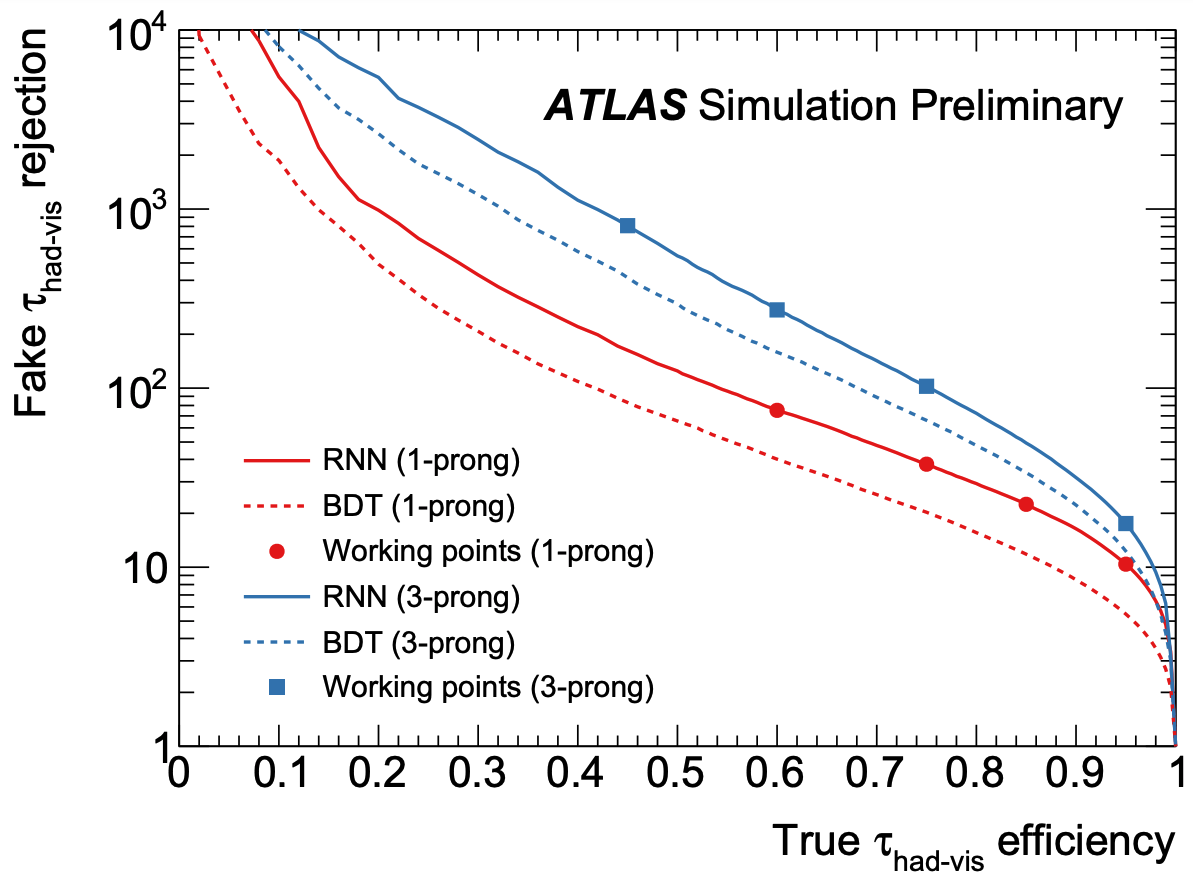
\includegraphics[width=0.75\textwidth]{FakeTau/BDT_vs_RNN}
\caption{Rejection power for jets misidentified as visible \htau\ (fake visible \htau) depending on the true visible \htau\
efficiency. Shown are the curves for 1-prong (red) and 3-prong (blue) visible \htau\ candidates using the \ac{RNN}-based (full
line) and the \ac{BDT}-based (dashed line) identification algorithms. The markers indicate the four defined working
points \textit{Tight, Medium, Loose and Very loose} with increasing signal selection efficiencies (taken from ~\cite{ATL-PHYS-PUB-2019-033}).}
\label{fig:BDTvsRNN}
\end{figure}

The rejection power against misidentified \htau\ as a function of the true visible \htau\ selection efficiency, for both \ac{BDT} and \ac{RNN} classifiers (independently for 1-prong and 3-prong candidates), is shown in Figure ~\ref{fig:BDTvsRNN}.
Four working points with increasing background rejection (\textit{Very loose}, \textit{Loose}, \textit{Medium} and\textit{Tight}) are used in the physics analyses. The corresponding signal selection efficiencies and rejection powers are given in Table \ref{tab:BDT_RNN_eff}
\begin{table}[!hbt]
\caption{List of defined working points with fixed true visible \htau\ selection efficiencies and the corresponding background rejection factors for misidentified visible \htau\ in multi-jet events for the \ac{BDT} and \ac{RNN} classifiers (taken from ~\cite{ATL-PHYS-PUB-2019-033}).}\label{tab:BDT_RNN_eff}
%\documentclass[10pt]{article}
%\usepackage[usenames]{color} %used for font color
%\usepackage{amssymb} %maths
%\usepackage{amsmath} %maths
%\usepackage[utf8]{inputenc} %useful to type directly diacritic characters
%\begin{document}
%\begin{table}[]
\resizebox{\textwidth}{!}{\begin{tabular}{lcccccc}
\hline 
              & \multicolumn{2}{c}{Signal Efficiency}                     & \multicolumn{2}{c}{Background Rejection BDT}              & \multicolumn{2}{c}{Background Rejection RNN}              \\
Working Point & \multicolumn{1}{c}{1-prong} & \multicolumn{1}{c}{3-prong} & \multicolumn{1}{c}{1-prong} & \multicolumn{1}{c}{3-prong} & \multicolumn{1}{c}{1-prong} & \multicolumn{1}{c}{3-prong} \\ \hline \hline
Tight         & 60\%                        & 45\%                        & 40                          & 400                         & 70                          & 700                         \\
Medium        & 75\%                        & 60\%                        & 20                          & 150                         & 35                          & 240                         \\
Loose         & 85\%                        & 75\%                        & 12                          & 61                          & 21                          & 90                          \\
Very Loose    & 95\%                        & 95\%                        & 5.3                         & 11.2                        & 9.9                         & 16                          \\ \hline
\end{tabular}}
%\end{table}
%
%\end{document}	
\end{table}

It is important to note that the rejection power for jets misidentified as visible \htau\ objects is strongly dependent on the reconstructed \htau\ \pt\ (as well more weakly dependent on $\eta$ and \mubar)~\cite{ATL-PHYS-PUB-2019-033}. 
Figure ~\ref{fig:BDT_RNN_rejection_power} shows the background rejection in multi-jet events for the \textit{Medium} working point for both \ac{BDT} and \ac{RNN} classifiers as a function of reconstructed \htau\ \pt. The rejection power is found to increase with increasing \pt. 
	\begin{figure}[!htb]
		\begin{center}
			\subbottom[]{
						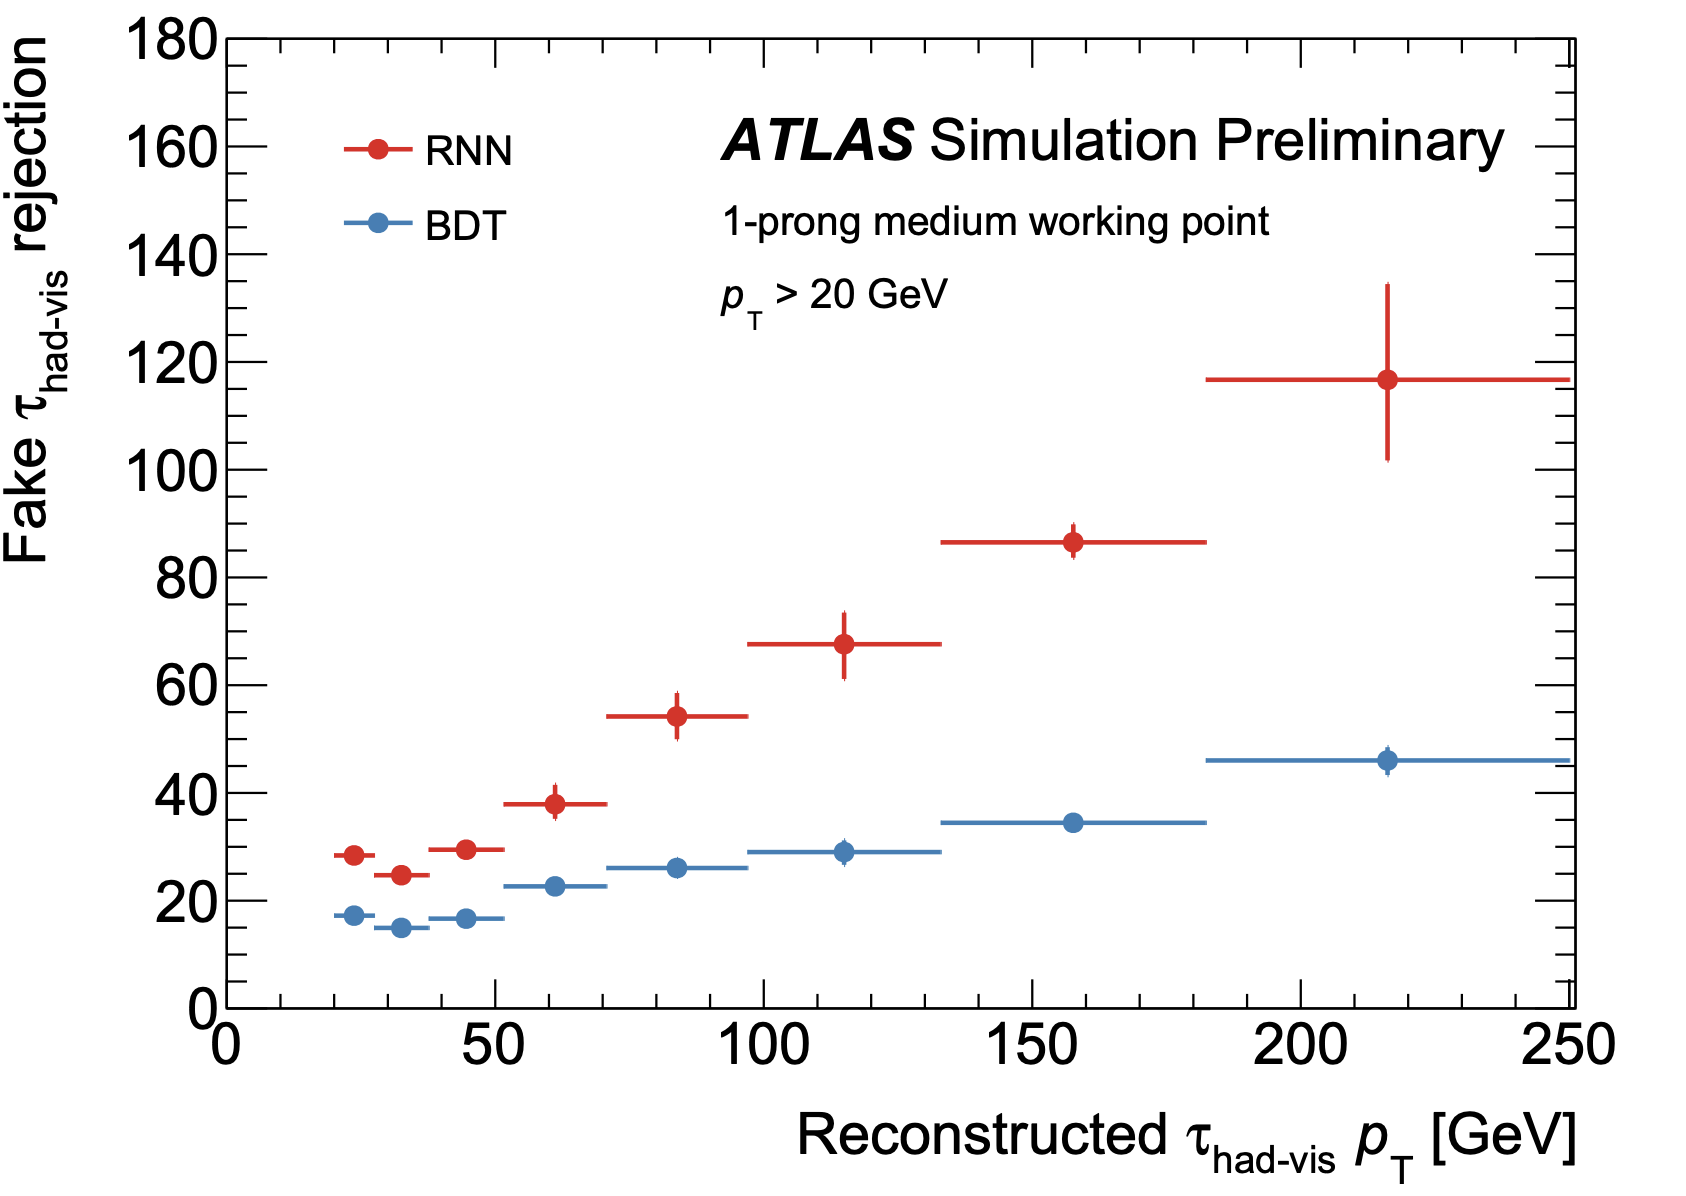
\includegraphics[width=0.45\textwidth]{FakeTau/BDT_RNN_rejection_power_1p}}\hspace{0.05\textwidth}
			\subbottom[]{
						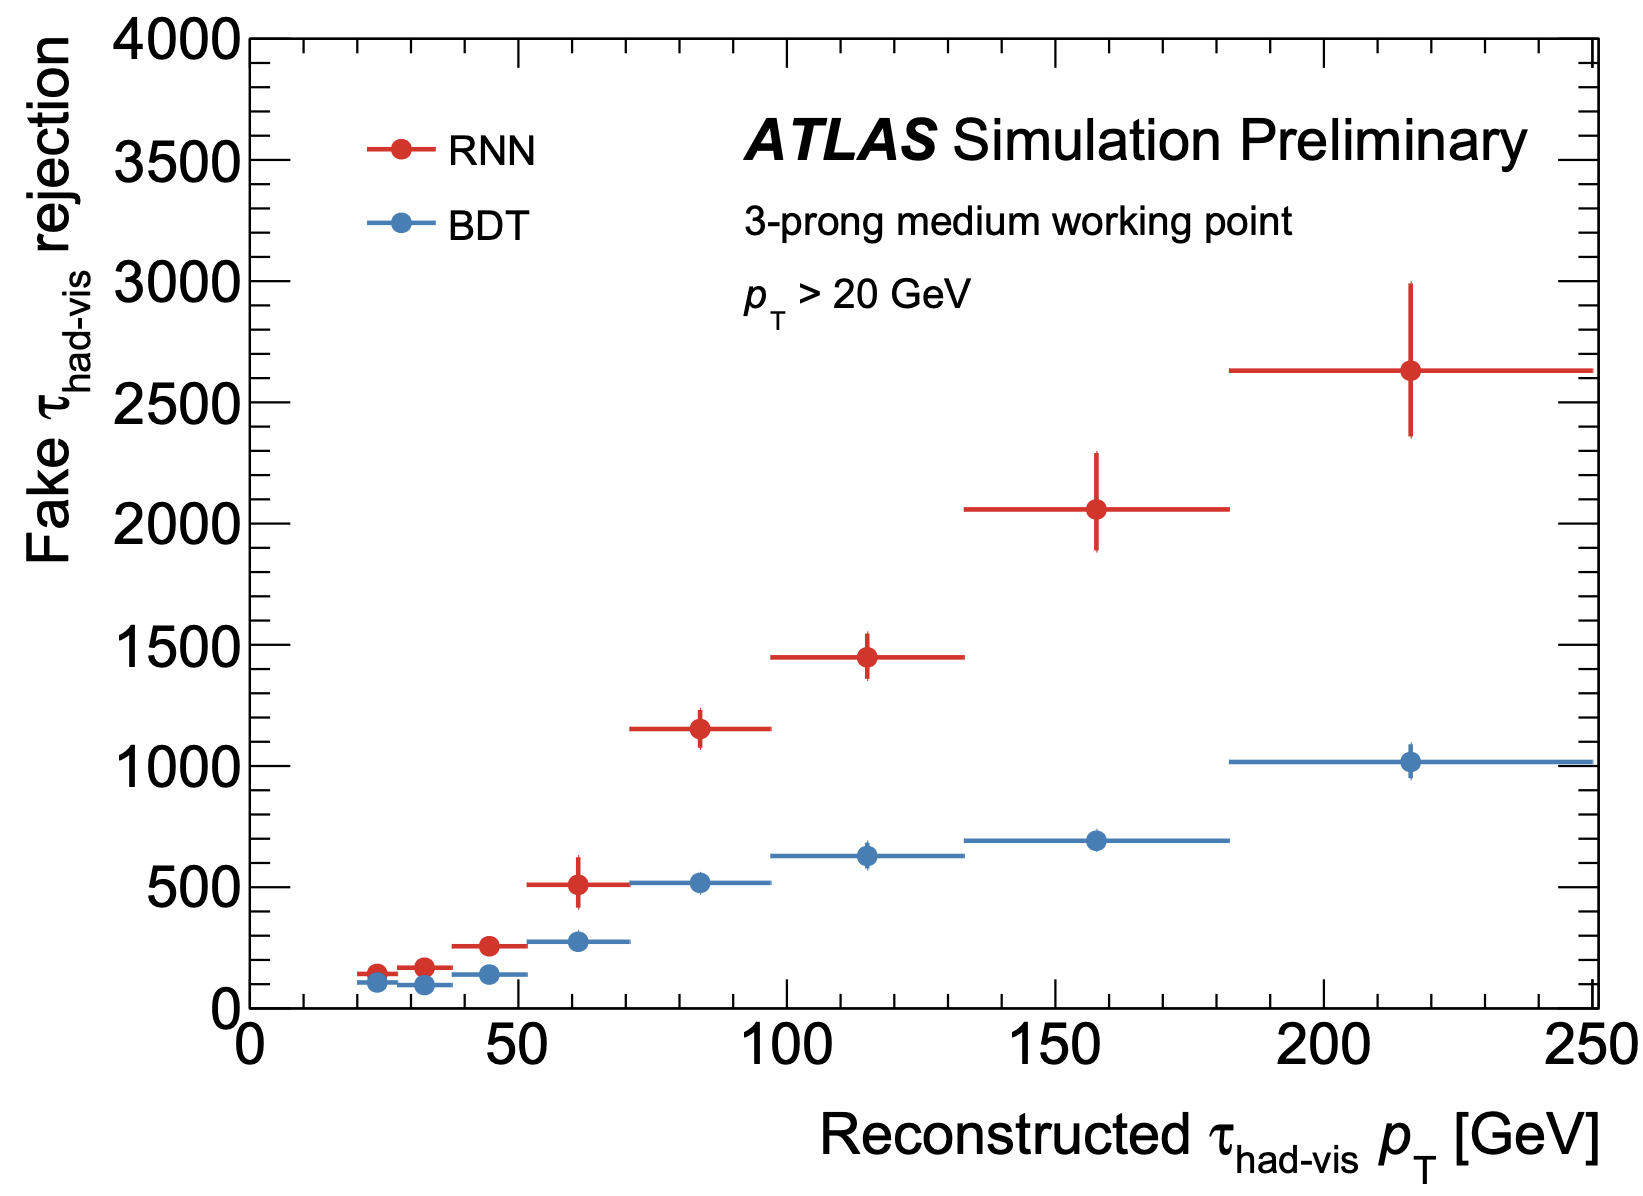
\includegraphics[width=0.45\textwidth]{FakeTau/BDT_RNN_rejection_power_3p}}\hspace{0.05\textwidth}
		\end{center}
		\caption{Rejection power for jets misidentified as visible \htau\ (fake visible \htau) for (a) 1-prong and (b) 3-prong as a function of their transverse momentum \pt. The rejection power is shown for the \textit{Medium} working point for both \ac{RNN}-based (red) and \ac{BDT}-based (blue) classifiers. (taken from ~\cite{ATL-PHYS-PUB-2019-033}).}
		\label{fig:BDT_RNN_rejection_power}
	\end{figure}

	\section{Trigger Strategy} 
	\label{sec:anatrig}
	In this section the triggers strategy used for the selection of relevant events for the search of the direct \stau\ production is presented. 
	%The study of the combined tau triggers \acp{SF} and efficiencies for use in the selection of relevant events in the \ac{SR} was performed by the author and is presented below. 
	%The trigger used for each \ac{SR}, along with the \textit{offline} (\ie\ data that has been collected and saved) selection applied to achieve high acceptance with low inefficiencies will be shown. 
	
	As discussed in Chapters ~\ref{ch:detector} and ~\ref{ch:trigger}	, physics events are only recorded if they pass a certain trigger with some \textit{online} (\ie\ during data taking) object kinematic threshold.
	In order to 	ensure high trigger efficiencies for the full range of the possible \ac{SUSY} kinematic regimes, the \ac{SR} is split into two separate and orthogonal regions based on \met. 
	Events with \met$>150$ \gev\ are triggers using the so-called \textit{di-tau+\met} trigger and target the high \stau\ mass region signature, as higher values of \met\ would be expected with for the higher \stau\ masses. For low \stau\ mass events, the expectation is that there would be lower \met\ values and thus events with \met$<150$ \gev\ are selected using the \textit{asymmetric di-tau} trigger.
	The use of these two triggers, along with the opposite \met\ requirement, ensures orthogonality of the selected events, thus removing the possibility of double counting events by the two triggers. 
	Because of changes to triggers and trigger menus throughout the Run-2 data taking period (2016-2018) the asymmetric di-tau and di-tau+\met\ triggers were changed in 2018.
	The most significant change occurred between 2017 and 2018 where the di-tau triggers were changed to use full tacking information instead of the fast tracking denoted by the \textit{tracktwoEF} nomenclature\footnote{Refer to Section~\ref{sec:Trig_intro} regarding the rules and structure used for trigger nomenclature.}.
	The lowest unprescaled triggers used for event selection in this analysis throughout the Run-2 data taking period can be found in Table~\ref{tab:analysis_triggers}.
	\begin{table}[!hbt]
	\centering
	\caption{Lowest unprescaled triggers for Run-2 with two hadronic taus (asymmetric di-tau) or two hadronic taus with missing transverse momentum (\met).}
	%\documentclass[10pt]{article}
%\usepackage[usenames]{color} %used for font color
%\usepackage{amssymb} %maths
%\usepackage{amsmath} %maths
%\usepackage[utf8]{inputenc} %useful to type directly diacritic characters
%\begin{document}
%\begin{table}[]
\resizebox{\textwidth}{!}{\begin{tabular}{c|c}
\hline 
Year & Trigger \\ \hline \hline
 & \textit{di-tau + $E_{T}^{miss}$} \\
2015-2017 & HLT\_tau25\_medium1\_tracktwo\_tau25\_medium1\_tracktwo\_xe50 \\
2018 & HLT\_tau60\_medium1\_tracktwoEF\_tau25\_medium1\_tracktwoEF\_xe50 \\ \hline
 & \textit{asymmetric di-tau} \\
2015-2017 & HLT\_tau80\_medium1\_tracktwo\_L1TAU60\_tau50\_medium1\_tracktwo\_L1TAU12 \\
2018 & HLT\_tau80\_medium1\_tracktwoEF\_L1TAU60\_tau60\_medium1\_tracktwo\_L1TAU40\\ \hline 
\end{tabular}}
%\end{table}
%
%\end{document}	
	\label{tab:analysis_triggers}
	\end{table}
	
	To properly model the efficiency of these combined object triggers on \ac{MC} simulations the \acp{SF} of these combined trigger objects are derived.
	 As discussed in Chapter ~\ref{ch:detector}, \ac{SF} are scaling factors derived from data and applied to the \ac{MC}, to match the performance observed in the data. 
	\subsection*{Efficiency}
	The trigger performance is parametrised by the efficiency of the trigger to select events of interest.  
	%To properly model the efficiency of these combined object triggers in both data and \ac{MC} simulations the \acp{SF} for the individual single objects triggers that constitute the full combined trigger, \textit{trigger legs}, are derived. As discussed in Chapter ~\ref{ch:detector}, \ac{SF} are scaling factors derived from data and applied to the \ac{MC}, to match the performance observed in the data. 
	For combined triggers such as the ones used in this analysis, the efficiency is defined as:
	\begin{equation}
		\epsilon = \frac{N_{\mathrm{S}}^{\mathrm{trig.}}}{N_{\mathrm{S}}},
		\label{eq:trig_eff}
	\end{equation}		
	where $N_{\mathrm{S}}$ is the number of events that pass some set of selection cuts for an arbitrary region, $S$, and  $N_{\mathrm{S}}^{\mathrm{trig.}}$ is the number of events that pass the same region selection and the trigger.
	To derive the efficiency of combined triggers  the individual trigger "legs" that constitute the full  trigger are considered to be independent. 
	The efficiency of the single legs of the combined triggers is, thus, derived using \ac{MC} simulations in a region defined to be abundant with the triggered object. 
	%For the asymmetric di-tau and di-tau+\met\ triggers used in this analysis,the single \ltau\ trigger leg that constitute the combined triggers online thresholds are: 25 \gev\, 35 \gev\, 50 \gev\, 60 \gev\, and 80 \gev.
	 Single \ltau\ triggers, representing the individual trigger legs that constitute the asymmetric di-tau and di-tau+\met\ triggers, with online thresholds of 25 \gev\, 35 \gev\, 50 \gev\, 60 \gev\, and 80 \gev, are used.
	These triggers are evaluated region abundant with W boson production in association with jets with \htau\ final states, as defined below:
%	\begin{itemize}
%	\item at least one medium \ltau\
%	\item one signal muon with \pt\ > 30 \gev\
%	\item \ltau\ and muon have opposite charged 
%	\item pass single muon trigger 
%	\item $65 < m(\mu,\tau) < 95$ \gev\
%	\item $b$-tagged jet events are rejected
%	\item $m_{T2}<$ 20 \gev\
%	\end{itemize}
	\begin{itemize}
	\item at least one medium \ltau\
	\item at least one jet with \pt\ > 100 \gev\
	\item \ltau\ and muon have opposite charged 
	\item pass \met\ trigger, \met\ > 200 \gev\
	\end{itemize}
	Using the above selection the transverse momentum distributions for the triggered and non-triggered tau are derived, as shown in Figure~\ref{fig:tau_single_leg_turnon} (so called \textit{turn on} curves).
	In these plots the \pt\ distributions for the leading tau object in each \ac{SM} samples are shown when using the different triggers. 
	Using equation ~\ref{eq:trig_eff}, the efficiency with respect to the non-triggered distribution is also shown in the bottom plot of the figures. 
	Vertical dashed lines are used to show offline thresholds that can be applied to ensure that the triggering is performed on the plateau of the efficiency distribution and thus where the trigger is at highest performance. 
	Higher online threshold triggers have lower offline thresholds to increase the acceptance in the higher \pt\ regions to improve statistics. 
	\singleTauTrigTurnOn
	
	The turn on curve for the single leg met trigger, with online energy threshold of 50 \gev, has been derived in a similar region as the one defined above but without any requirements on the \met.
	 For these distribution the turn on is found to be around 200 \gev.  
	These distributions can, however, only be used for reference and to evaluate the effect of the \met\ trigger on the \met\ kinematics distribution.
	Unfortunately they cannot be used to determine the efficiency of the \met\ trigger leg used in the di-tau+\met\ trigger because it should be derived in a region that is abundant with missing transverse energy originating from the \ltau\ decay process.
	The higher turn on threshold value seen in these distributions is a consequence of triggering on \met\ originating from decay processes with one \ftau\ object and \met\ originating from the decay process itself (\eg\ $Z\rightarrow\mu\nu_{\mu}$). 
	 \metTrigTurnOn
	 
	 To study the performance of the \met\ trigger a new region to isolate the $W\rightarrow\tau\nu_{\tau}$ decay process is defined using the following selection:
	 \begin{itemize}
	 \item one medium \ltau\
	 \item no light leptons ($e,\mu$)
	 \item no $b$-tagged jets
	 \item $m(\tau,E_T^{miss})\,>\,70$ \gev\	
	 \item \met\ > 120 \gev\
	 \end{itemize}
	 The invariant mass requirement between the \met\ and \ltau\ is used to select events from the \Wjets\ decay process, as mentioned previously. A \met > 120 \gev\ requirement is used to also remove events from other \ac{SM} background processes, which is possible to do in part due to the fact that only a small amount of performance will be lost, because of the large inefficiency of \met\ triggers at low missing transverse momentum values, as seen in Figure~\ref{fig:mettrig_turnon}. 
	%To check the efficiency of the prescaled \met\ trigger leg, a \textit{tag and probe method} is used. 
	Due to the inherent bias in the number of total events of the prescaled \met\ trigger leg, a \textit{tag and probe method} must be used to check the efficiency.
	%The tag and probe method is used to study the efficiency of any prescaled trigger, which has an inherit bias in the number of total events. 
	In the tag and probe method an orthogonal unprescaled trigger is used to select the relevant events (known as the \textit{tag trigger}). The prescaled trigger in question (known as \textit{probe trigger}), is then checked to see if it has also triggered for the selected event. 
	The efficiency for the tag and probe method is then calculated as the ratio of probed events over the number of events that have been tagged: 
	\begin{equation}
	\epsilon=\frac{N_{T\&P}}{N_{P}}.
	\label{eq:TnP_eff}
	\end{equation}
	For this analysis a known unprescaled single tau trigger (\textit{tag}) is used to select relevant events. 
	The \met\ trigger is then checked to see if it has also been fired (\textit{probe}) in these events. 
	A 160 \gev\ online threshold single tau trigger is used as the probe trigger with an offline \pt\ > 180 \gev\ requirement to ensure that events on the trigger plateau are selected. 
	 Figure~\ref{fig:TnP_kine} shows the \ltau\ \pt\ and \met distributions for the events that pass the tag and probe selection in this region.
	 \ac{MC} simulated \ac{SM} background processes are used to evaluate the kinematic distribution of data.
	  The simulated background processes and data distributions are found to have good agreement, with the \Wjets\ as the main contributing background process. 
	 \metTrigKine
	 
	 Using Equation~\ref{eq:TnP_eff} the trigger efficiencies in both the combined \ac{SM} background samples and collected data can be derived, as shown by the bottom plot of Figure~\ref{fig:TnP_eff}, while the top plots shows the number of events that pass the tag (black) and tag+probe (tag+probe) trigger requirements as a function of transverse missing energy, respectively.
	 The efficiency exceeds 90\% in both data and background at around 150 \gev\ (shown by red dotted line), above which it quickly increases to 100\% for higher \met\ values. 
	 \metTrigEff
	 Using derived trigger efficiencies the \met\ trigger \ac{SF} are derived, as shown in Figure~\ref{fig:TnP_SF}, for the range of \met\ values above 120 \gev.
	 The \ac{SF} are found to be approaching unity for large \met\ values, thus indicating \ac{MC} simulations to be a good at estimating for the performance of the \met\ trigger in data. Because of changes in the trigger menu between data collection years, the simple \met\ trigger was only turn on for data collected in 2016, and was not available for the data collected in the later years.
	 \metTrigSF
	 
	To ensure that the combined triggers are performing at maximal efficiency offline selections cuts for the triggered objects are used to select the event that lie on the plateau of the trigger turn on curve.
	 %To ensure that the events selected by the combined triggers are performing on the plateau of the efficiency distribution, offline selections cuts for the triggered objects are used. 
	 For the di-tau+\met\ trigger an offline  50 \gev\ minimum \pt\ requirement on the highest \ltau\ is used for data collected between 2015-2017, which was increased to 75 \gev\ in 2018 due to the change of triggers, while the second triggered \ltau\ in the event is required to have \pt\ > 40 \gev. An offline requirement of \met\ > 150 \gev\ is used for the \met\ leg of the combined trigger. 
	 For the asymmetric di-tau trigger the highest energy \ltau\ of the event is required to have an offline \pt\ > 95 \gev, while the second highest energy \ltau\ must have \pt\ > 60 (75) \gev\ for data collected between 2015-2017 (2018). 
	 The online (\ac{HLT}) and offline thresholds used by each trigger for each trigger leg are summarised in Table~\ref{tab:analysis_trig_thresh}.
	 
	 \begin{table}[!hbt]
	 \centering
	\caption{Lowest unprescaled triggers for Run-2 with two hadronic taus (asymmetric di-tau) or two hadronic taus with missing transverse momentum (\met).}
	
\begin{tabular}{ccccc}
\hline 
Trigger & Trigger leg & Year & \begin{tabular}[c]{@{}c@{}}HLT\\ {[}GeV{]}\end{tabular} & \begin{tabular}[c]{@{}c@{}}Offline\\ {[}GeV{]}\end{tabular} \\ \hline \hline
\multirow{4}{*}{di-tau+$E_T^{\mathrm{miss}}$} & \multirow{2}{*}{leading $\tau$-lepton $p_T$} & 2015-2017 & 35 & 50 \\
 &  & 2018 & 60 & 75 \\
 & 2nd leading $\tau$-lepton $p_T$ & 2015-2018 & 25 & 40 \\
 & $E_T^{\mathrm{miss}}$ & 2015-2018 & 50 & 150 \\ \hline
\multirow{3}{*}{asymmetric di-tau} & leading $\tau$-lepton $p_T$ & 2015-2018 & 80 & 95 \\
 & \multirow{2}{*}{2nd leading $\tau$-lepton $p_T$} & 2015-2017 & 50 & 60 \\
 &  & 2018 & 60 & 75 \\ \hline
\end{tabular}


	
	\label{tab:analysis_trig_thresh}
	\end{table}
	 
	\subsection*{Triggers independence test}
	The individual trigger legs of a combined trigger are considered to be independent. 
	The efficiency of the full trigger can, thus, be derived by combining the trigger efficiencies of the individual legs of which is constituted. 
	This assumption is tested and proved using a \textit{closure test}.
	The closure test is performed, using \ac{MC} simulated samples, by comparing the product of the efficiencies of the two legs with the trigger efficiency of the full di-tau trigger.
	For this closure test the asymmetric di-tau trigger as well as the combined di-tau legs of the di-tau+\met\ trigger are tested with respect to their corresponding single tau trigger legs:
	\begin{description}
	\item[tau80\_tau50:] HLT\_\textbf{tau80}\_medium1\_tracktwo\_L1TAU60\_\textbf{tau50}\_medium1\_tracktwo\_L1TAU12
	\item[tau80\_tau60:] HLT\_\textbf{tau80}\_medium1\_tracktwoEF\_L1TAU60\_\textbf{tau60}\_medium1\_tracktwoEF\_L1TAU40
	\item[tau35\_tau25:] HLT\_\textbf{tau35}\_medium1\_tracktwo\_\textbf{tau25}\_medium1\_tracktwo\_2TAU12IM
	\end{description}	
	A simple selection of 2 medium \ac{OS} \ltau s with no $b$-tagged jets, nor light leptons in the event is used. 
	Figure~\ref{fig:tau_single_leg_closure} shows the resulting efficiencies, as defined by Equation~\ref{eq:trig_eff} for the single legs and combined triggers using this selection. The bottom plot of the figures show the closure test, which is found to be close to unity for \ltau\ \pt\ values above 90 \gev\  for the asymmetric di-tau trigger. Similarly, the di-tau leg of the di-tau+\met\ is also fond to have a closure test value of approximately one for the full range of \pt\ values above 50 \gev.
	Therefore the closure test shows that the single trigger legs can be combined to give the total efficiencies of the di-tau triggers for values above the offline trigger thresholds. 
	\ditauClosureTest
	%\subsection*{Scale factors}
	\section{Event Selection}
	\label{sec:evtsel}
	The analysis presented utilises a cut-and-count strategy to isolate the \ac{SUSY} signal from the \ac{SM} background, using dedicated sets of discriminating variables. 
	Background-enriched regions, defined as \acp{CR} are used to estimate the contribution of the most relevant background in the defined \ac{SR}.
	\ac{MC}-based or data-driven methods can be used to estimate the relative contribution of background in the \ac{SR},depending on the process that is being estimated. 
	A detailed description of the background estimation methods used in this analysis can be found below. 
	
	Due to the different running conditions and configurations of the detector, some selection (\eg\ trigger requirements or calibration parameters) are applied differently between data collected in 2015 to 2018. The different selections used in the selection of relevant events will be discussed in more details in Sections ~\ref{subsec:SRopt} and ~\ref{subsec:CRest}.
	\ac{MC} samples are generated for various periods of data taking, where a random number that identified a given \ac{ATLAS} run is generated and associated to the simulated \ac{MC} event. This way simulated events can be associated with specific operation periods that reflect the parameters with which data was collected. 
	
	\subsection{Event Cleaning}
	\label{subsec:evntcleaning}
	%Faults in the \ac{ATLAS} detector during data taking can occur. In order to remove these unwanted events a set of offline (not in real time) cuts is applied to clean the event sample used.  
	Event cleaning requirements are applied to data to ensure that only events collected when the detector was fully functional are used in the analysis.
	The first requirement for the event to be accepted as \textit{"good physics"} is for the existence of a primary vertex with a minimum of two tracks, with \pt\ $>$ 400 \mev, associated to it. 
	The status of the \ac{HCAL} and \ac{ECAL} is also checked and if any error state is returned the event is discarded.
	To reduce and suppress the fake-jet (\textit{bad jet}) contamination, quality requirements on a variety of jet parameters are checked. 
	These parameters include the fraction of energy deposited in the different layers of the calorimeters, and the fraction of jet \pt\ measured by the tracks in the \ac{ID}. 
	Events containing bad jets that pass \ac{OR} are discarded. 
	Events containing muon candidates whose relative uncertainty on $e/p$ is larger than 20\%, or that have been identified as not originating from the $pp$ collision (cosmic), are also discarded. 
	\subsection{Signal Regions and optimization}
	\label{subsec:SRopt}
	The experimental signature expected for the signal topology described in Section ~\ref{sec:susysig}  is the presence of two taus that have decayed fully hadronically and a significant amount of \met. 
	No additional jets or light leptons (electrons or muons) in the signal event final state are expected.
	
	As explained in Section ~\ref{sec:anatrig}, in order to use the tau trigger \ac{SF}s and efficiencies from the individual triggers, two orthogonal \ac{SR} are constructed:
	\begin{description}
	
	\item[Low-mass SR:] Optimised to cover the low stau mass processes. The asymmetric di-$\tau$ trigger in events with \met\ $\leq$ 150 \gev is used.
	\item[High-mass SR:] Targets the high stau mass processes, using the di-$\tau+$\met\ trigger in events with \met\ $>$ 150 \gev.
	\end{description}	 
	\subsection*{Preliminary selection and discriminating variables}
	The preliminary selection (\textit{pre-selection}) is a basic selection common to both \ac{SR}s, used as an initial step to separate the signal from the backgrounds. 
	This selection includes the common event cleaning described in Section ~\ref{subsec:evntcleaning} and the trigger selection described in Section ~\ref{sec:anatrig}. 
	A further selection is applied where events are selected if they contain exactly two medium taus after \ac{OR}. 
	The two selected taus are required to be of opposite charge, generally referred to as \ac{OS} taus, and to be matched to the corresponding trigger objects at \ac{HLT} level, and apposite requirement on the offline \met\ and tau transverse momenta are applied to ensure that the triggers are in their efficiency plateau. 
	If light leptons, a third tau, or a b-jet are present, the event is rejected to ensure orthogonality from the semi-hadronic channel (where one tau decays to leptons), to suppress 3 tau background processes, and to suppress \ac{SM} backgrounds originating from top quarks.
	Events with invariant mass of the two visible taus below 120 \gev\ are rejected to suppress contribution from the \Zjets and Higgs \ac{SM} background events (Z/H veto). The summary of the used pre-selection is shown in table ~\ref{tab:analysis_preselection}.
	
	\begin{table}[!hbt]
	\centering
	\caption{Preliminary selection common to both low- and high-mass \ac{SR} in addition to the event cleaning.}
	%\documentclass[10pt]{article}
%\usepackage[usenames]{color} %used for font color
%\usepackage{amssymb} %maths
%\usepackage{amsmath} %maths
%\usepackage[utf8]{inputenc} %useful to type directly diacritic characters
%\begin{document}
%\begin{table}[]
%\resizebox{\textwidth}{!}{
\begin{tabular}{cc}
\hline 
\multicolumn{1}{c}{Low-mass Preselection} & High-mass Preselection \\ \hline \hline
\multicolumn{2}{c}{2 medium taus (OS)} \\
\multicolumn{2}{c}{light lepton veto and 3rd tau veto} \\
\multicolumn{2}{c}{b-jet veto} \\
\multicolumn{2}{c}{Z/H-veto ($m(\tau_1,\tau_2)\,>\,120$ GeV)} \\ 
\multicolumn{1}{c|}{asymmetric di-tau trigger} & di-tau+$E_T^{miss}$ trigger \\
\multicolumn{1}{c|}{$E_T^{miss}\,\leq$ 150 GeV} & $E_T^{miss}\,>$ 150 GeV \\
\multicolumn{2}{c}{$\tau_1$ and $\tau_2$ $p_T$ trigger requirements} \\ \hline 
\end{tabular}
%}

%\end{table}
%
%\end{document}	
	\label{tab:analysis_preselection}
	\end{table}
	The following event kinematic variables or global event properties, based on the decay topology of \ac{SUSY}, top, and Z events are studied to further select signal events:
	\begin{description}
	%\item [\boldmath $m_T:$] the transverse mass of the leading ($m_{T,\tau_1}$) and sub-leading  ($m_{T,\tau_2}$) tau objects in the event defined by
	% $$ m_{T}(\textbf{p}_T,\textbf{q}_T)\,=\,\sqrt{2(p_Tq_T-\textbf{p}_T\cdot\textbf{q}_T)} $$
	%where $p_T$ and $q_T$ are the transverse momenta and the transverse vector that minimises the mar
	\item [\boldmath $M_{T2}:$] \textit{stranverse mass}, which can be shown to have a kinematic endpoint for events where two massive pair produced particles decay to two objects, one of which is detected and the other escapes undetected~\cite{LESTER199999,Barr:2003rg}. In the case of this analysis, the detected object is the visible tau while the undetected object is the neutralino.
	The stransverse mass is defined as:
	$$ m_{T2}\,=\,\underset{\textbf{q}_T}{\mathrm{min}}\left[\mathrm{max}\left(m_{T,\tau_1}(\textbf{p}_{T,\tau_1},\textbf{q}_T),m_{T,\tau_2}(\textbf{p}_{T,\tau_2},\textbf{q}_T)\right)\right],$$
	where $\textbf{p}_{T,\tau_1}$ and $\textbf{p}_{T,\tau_2}$ are the transverse momenta of the two leading tau, and  $\textbf{q}_T$ is the transverse vector that minimises the larger of the two transverse masses $m_{T,\tau_1}$ and $m_{T,\tau_2}$. The transverse momenta is thus defined:
	$$ m_{T}(\textbf{p}_T,\textbf{q}_T)\,=\,\sqrt{2(p_Tq_T-\textbf{p}_T\cdot\textbf{q}_T)};$$
	\item [\boldmath $m_{T,\tau_1}+m_{T,\tau_2}:$] the sum of the transverse mass values of the leading and next-to-leading taus;
	\item [\boldmath $M_{eff}:$] the \textit{effective mass} is the scalar sum of the missing transverse energy (\met) and the transverse momenta of the leading and next-to-leading taus;
	\item [\boldmath $\Delta R(\tau_1,\tau_2):$] the cone size between the leading and next-to-leading tau. An upper cut on this variable is a powerful discriminant against back-to-back events such as multi-jets;
	\item [\boldmath $m(\tau_1,\tau_2):$] the invariant mass of the two reconstructed taus.
	\end{description}
	
	\subsection*{Optimization strategy}
	The \ac{SR} optimization is fundamental for any analysis that uses the cut-and-count method. The goal is to remove as much background events as possible while retaining the largest possible number of signal events. The set of discriminating variables described above are used to this end.
	
	To represent the discovery significance of the signal model targeted, a \ac{FoM} is employed. 
	In this analysis the \ac{FoM} used is the \textit{significance}, which is the probability that an observed event counted in a \ac{SR} could have been produced by the sole fluctuation of the background in that region.
	The optimization of the cuts that comprise the \ac{SR} of interest is performed by maximising the value of the significance $Z_n$~\cite{Zn}, which is generally implemented in the \verb+RooStats+~\cite{2010acat.confE..57M} package within the \verb+ROOT+~\cite{Brun:1997pa} framework, and is defined as:
	\begin{equation}
	Z_n\,=\,\frac{N_{\textrm{sig}}}{\sqrt{N_{\textrm{bkg}}+(N_{\textrm{bkg}}\sigma_{\textrm{bkg}})^2}},
	\end{equation}
	where $N_{\textrm{sig}}$ and $N_{\textrm{bkg}}$ are the signal and background yields, respectively. $\sigma_{\textrm{bkg}}$ is the relative systematic uncertainty on the background which has been set to a flat 30\% based on previous analyses. Signal statistical uncertainty is not taken into account, as it is assumed to be negligible compared to the background uncertainty.   
	
	To avoid potential bias on the part of the analysers during the \ac{SR} optimization a so-called \textit{blinding} procedure is employed. 
	The number of data events that fall within the \ac{SR} is purposefully hidden from the analysers, until the modelling of the background falling into that \ac{SR} has been solidly estimated from background-enriched \acp{CR} and tested in \acp{VR}. The estimation and validation of the background is discussed in detail in Section ~\ref{subsec:CRest}.
	\subsection*{SR definition}
	Based on the optimization procedure described above, the optimised signal regions are defined in Table~\ref{tab:analysis_SR}. Values of \met > 75 \gev\ are required for the Low-mass \ac{SR} to increase signal sensitivity. In addition the two $\tau$-lepton candidates are required to satisfy $\Delta R(\tau_1,\tau_2)\,<\,3.2$, $|\Delta\phi(\tau_1,\tau_2)|\,>\,0.8$ and $m_{T2}\,>\,70$ \gev\ to further suppress contributions from \ac{SM} background processes. 
	%The product of acceptance and efficiency is around 0.04\% (0.03\%) and 0.53\% (1.22\%) for the reference points with \stau\ masses of 120 \gev\ and 280 \gev\, respectively, and \nino\ mass of 1 \gev\ in Low-mass \ac{SR} (High-mass \ac{SR})
		
	\begin{table}[!hbt]
	\centering
	\caption{Optimised selection for Low-mass and High-mass \acp{SR}.}
	%\documentclass[10pt]{article}
%\usepackage[usenames]{color} %used for font color
%\usepackage{amssymb} %maths
%\usepackage{amsmath} %maths
%\usepackage[utf8]{inputenc} %useful to type directly diacritic characters
%\begin{document}
%\begin{table}[]
%\resizebox{\textwidth}{!}{
\begin{tabular}{cc}
\hline 
Low-mass SR & High-mass SR \\ \hline \hline
\multicolumn{1}{c|}{2 tight $\tau$ (OS)} & 2 medium $\tau$ (OS), $\geq\,1$ tight $\tau$ \\
\multicolumn{2}{c}{light lepton veto and 3rd medium $\tau$ veto} \\
\multicolumn{2}{c}{$b$-jet veto} \\
\multicolumn{2}{c}{Z/H-veto ($m(\tau_1,\tau_2)\,>\,120$ GeV)} \\
\multicolumn{2}{c}{$|\Delta\phi(\tau_1,\tau_2)>0.8|$} \\
\multicolumn{2}{c}{$\Delta R(\tau_1,\tau_2)<3.2$} \\
\multicolumn{2}{c}{$m_{T2}>70$ GeV} \\  
\multicolumn{1}{c|}{asymmetric di-tau trigger} & di-tau+$E_T^{miss}$ trigger \\
\multicolumn{1}{c|}{$75\,<\,E_T^{miss}\,\leq$ 150 GeV} & $E_T^{miss}\,>$ 150 GeV \\
\multicolumn{2}{c}{$\tau_1$ and $\tau_2$ trigger $p_T$ requirements} \\ \hline
\end{tabular}
%}

%\end{table}
%
%\end{document}	
	\label{tab:analysis_SR}
	\end{table}
	The so-called "N-1" plots, showing the distributions of relevant kinematic variables, after the Low-mass and High-mass \acp{SR} requirements, except for shown variable, are shown in Figures~\ref{fig:SRL_analysis_N_1} and ~\ref{fig:SRH_analysis_N_1}, respectively. 
	%These plots kinematic variables that have been added to the blinded \acp{SR} to improve the signal sensitivity. 
	The red arrow shows the kinematic region that is accepted by the selection, while the rest is rejected.
	\begin{figure}[!hbt]
	\begin{center}
			\subbottom[$m_{T2}$ ($m_{T2}\,>\,70\,$ GeV)]{
				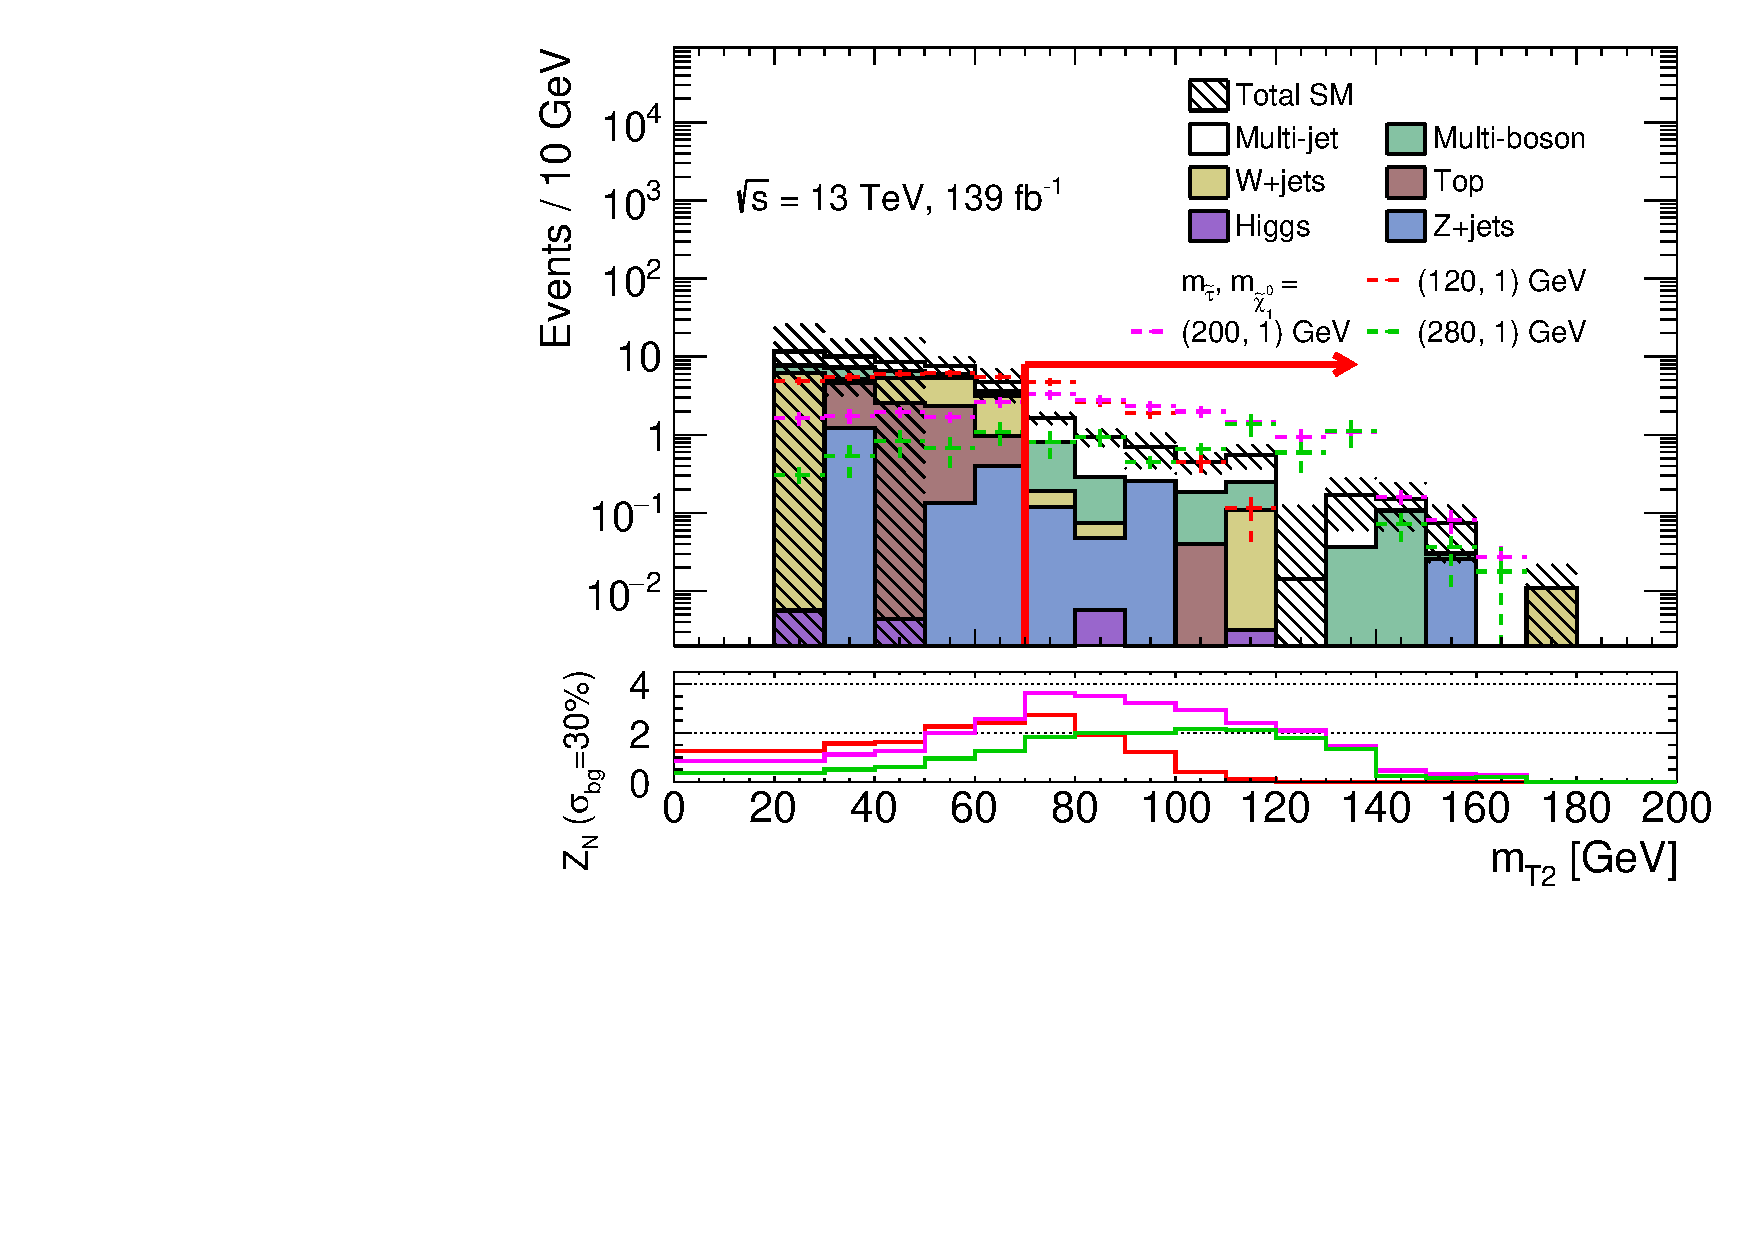
\includegraphics[width=0.4\textwidth]{Analysis/SRL/mT2_N_1}}\hspace{0.05\textwidth}	 
			 \subbottom[\met ($75\,<\,E_T^{miss}\,<\,150\,$ GeV)]{
				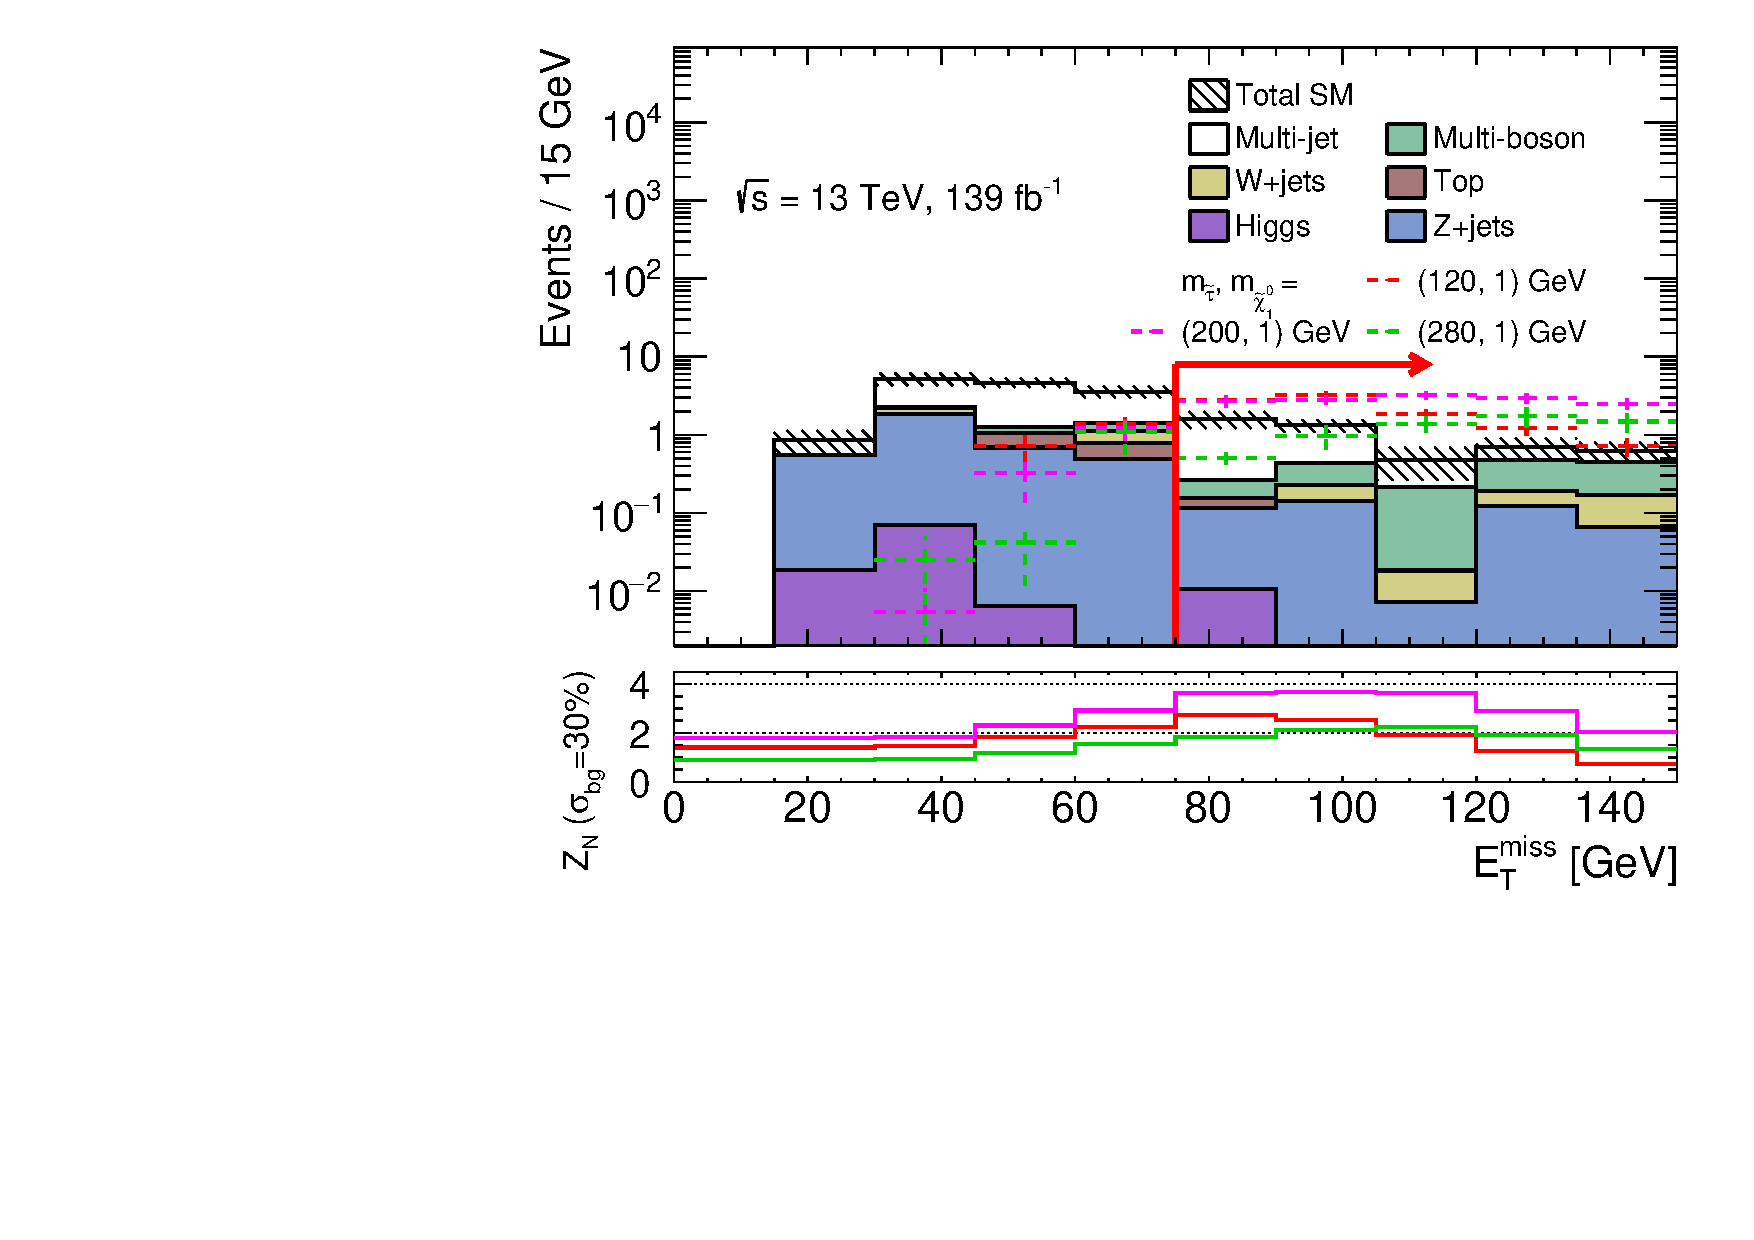
\includegraphics[width=0.4\textwidth]{Analysis/SRL/Evt_MET_N_1}}\hspace{0.05\textwidth}
			\subbottom[$\Delta R(\tau_1,\tau_2)$ ($\Delta R (\tau_1,\tau_2)\,<\,3.2$)]{
				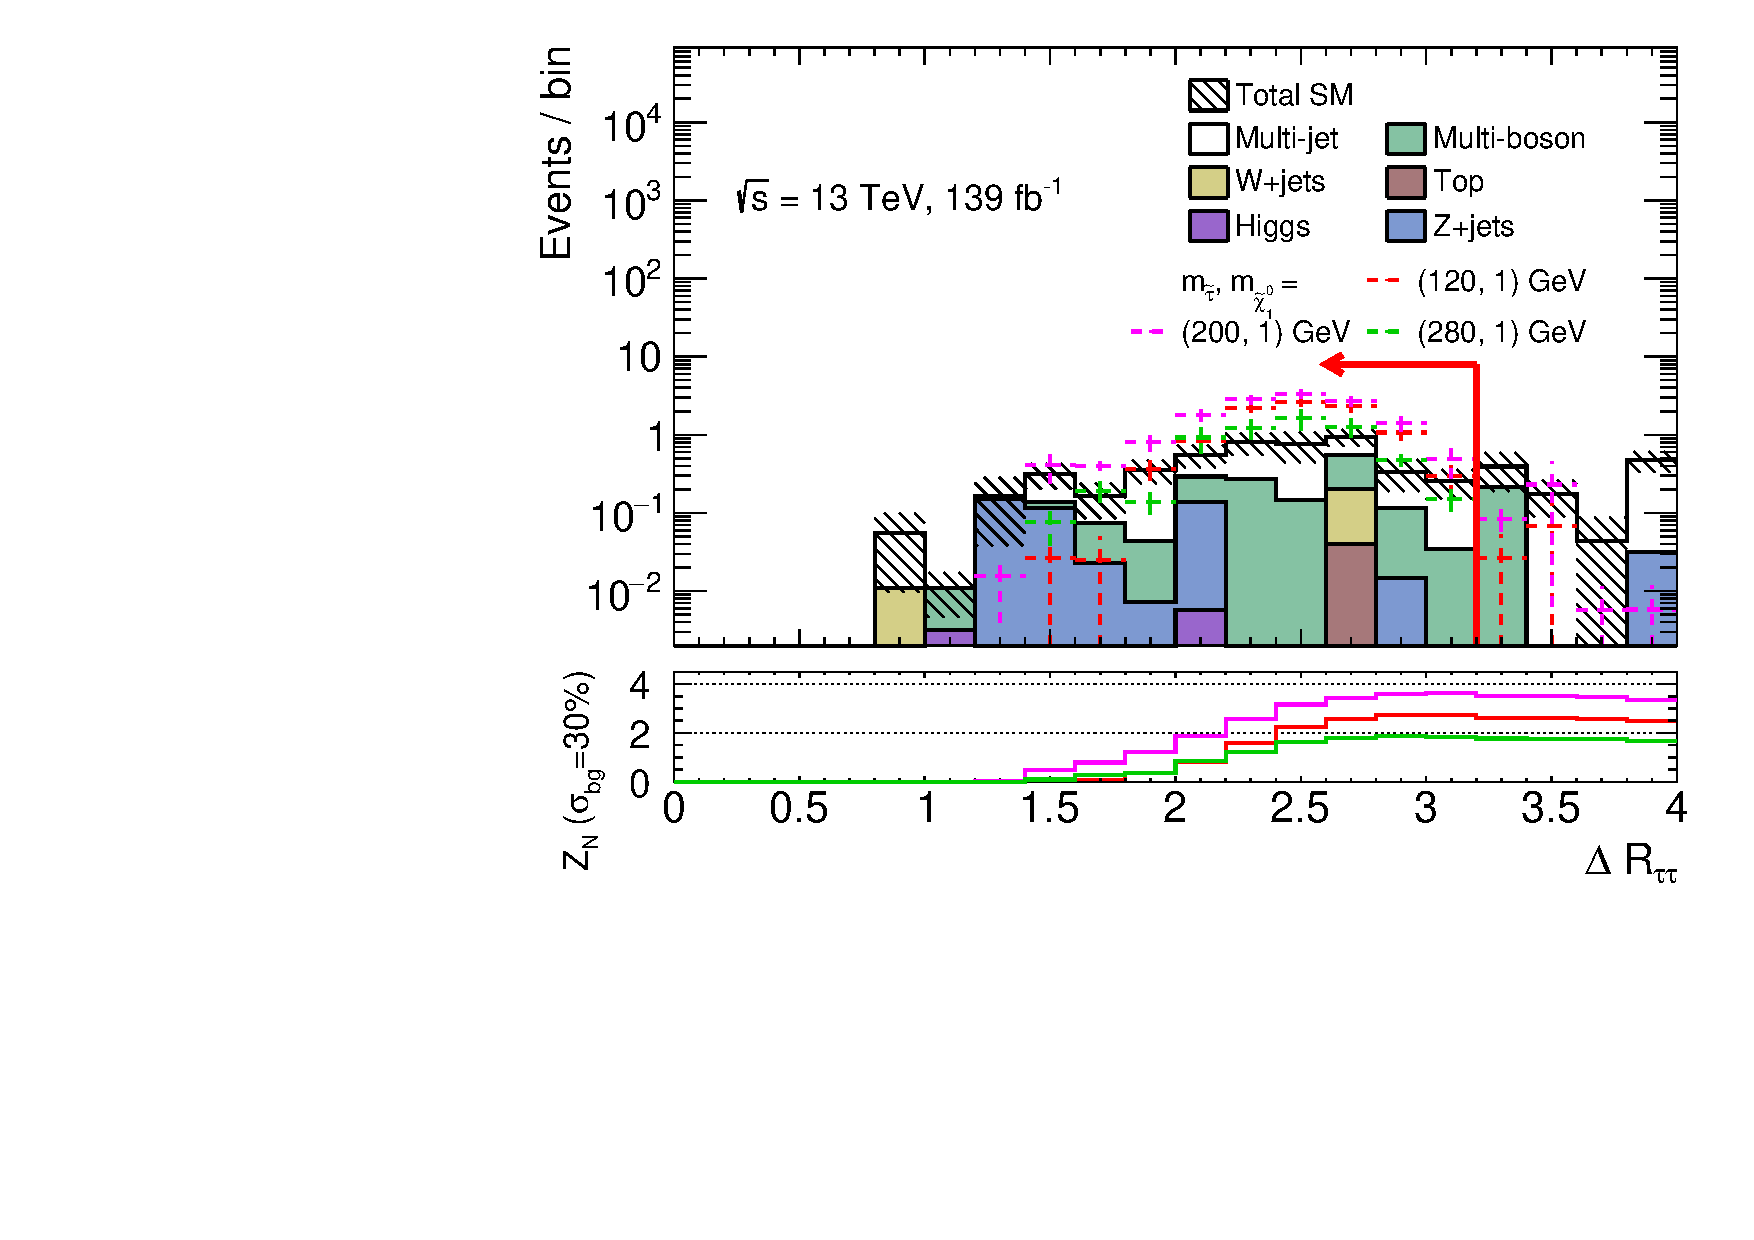
\includegraphics[width=0.4\textwidth]{Analysis/SRL/DRtt_N_1}}\hspace{0.05\textwidth}	 
			 \subbottom[$|\Delta\phi(\tau_1,\tau_2)|$ ($|\Delta\phi(\tau_1,\tau_2)|\,>\,0.8$)]{
				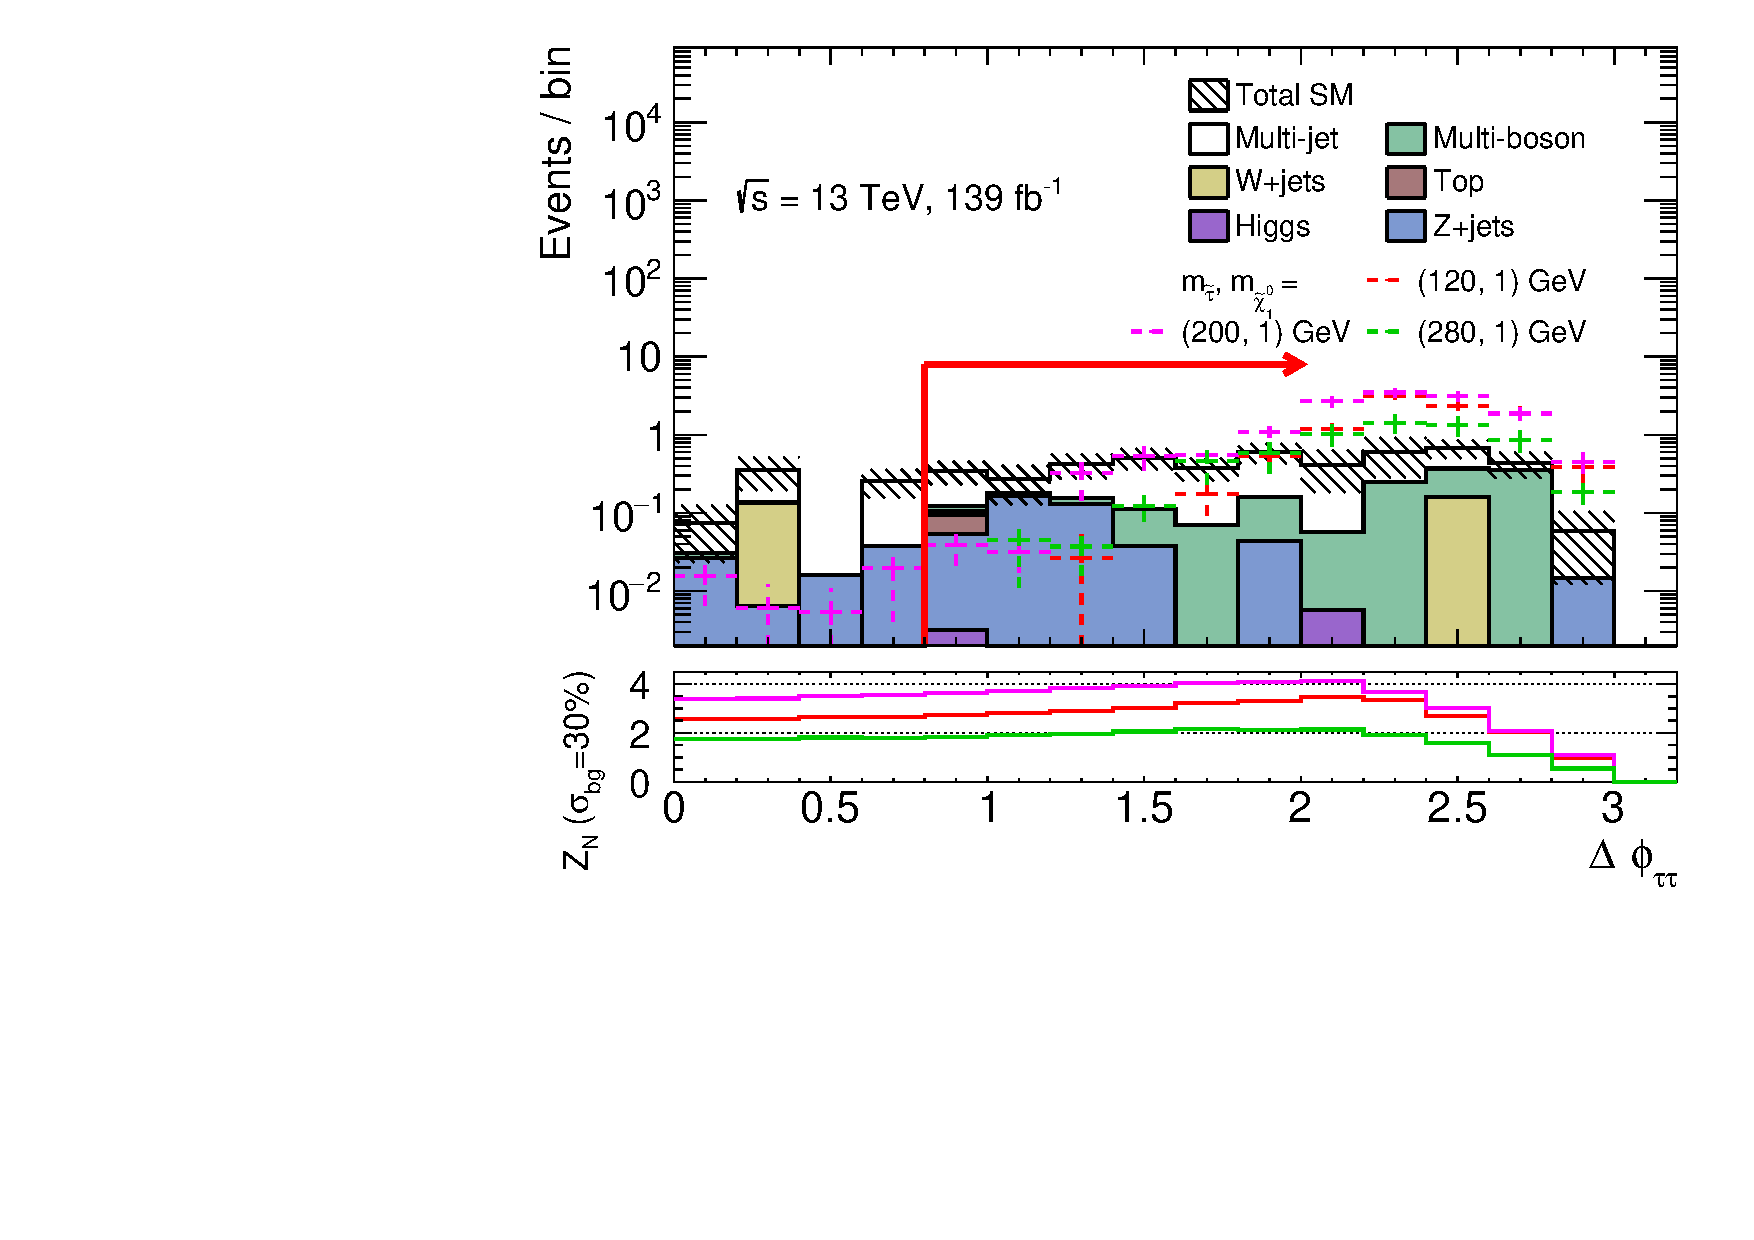
\includegraphics[width=0.4\textwidth]{Analysis/SRL/DPhitt_N_1}}\hspace{0.05\textwidth}
		\end{center}
		\caption{"N-1" distributions of relevant kinematic variables after Low-mass \ac{SR} requirements, except the one on the shown variable, are applied. The stacked histogram show the expected \ac{SM} background estimates from \ac{MC} normalised to 139 fb$^{-1}$.}
	\label{fig:SRL_analysis_N_1}
	\end{figure}	
	 
	 \begin{figure}[!hbt]
	\begin{center}
			\subbottom[$m_{T2}$ ($m_{T2}\,>\,70\,$ GeV)]{
				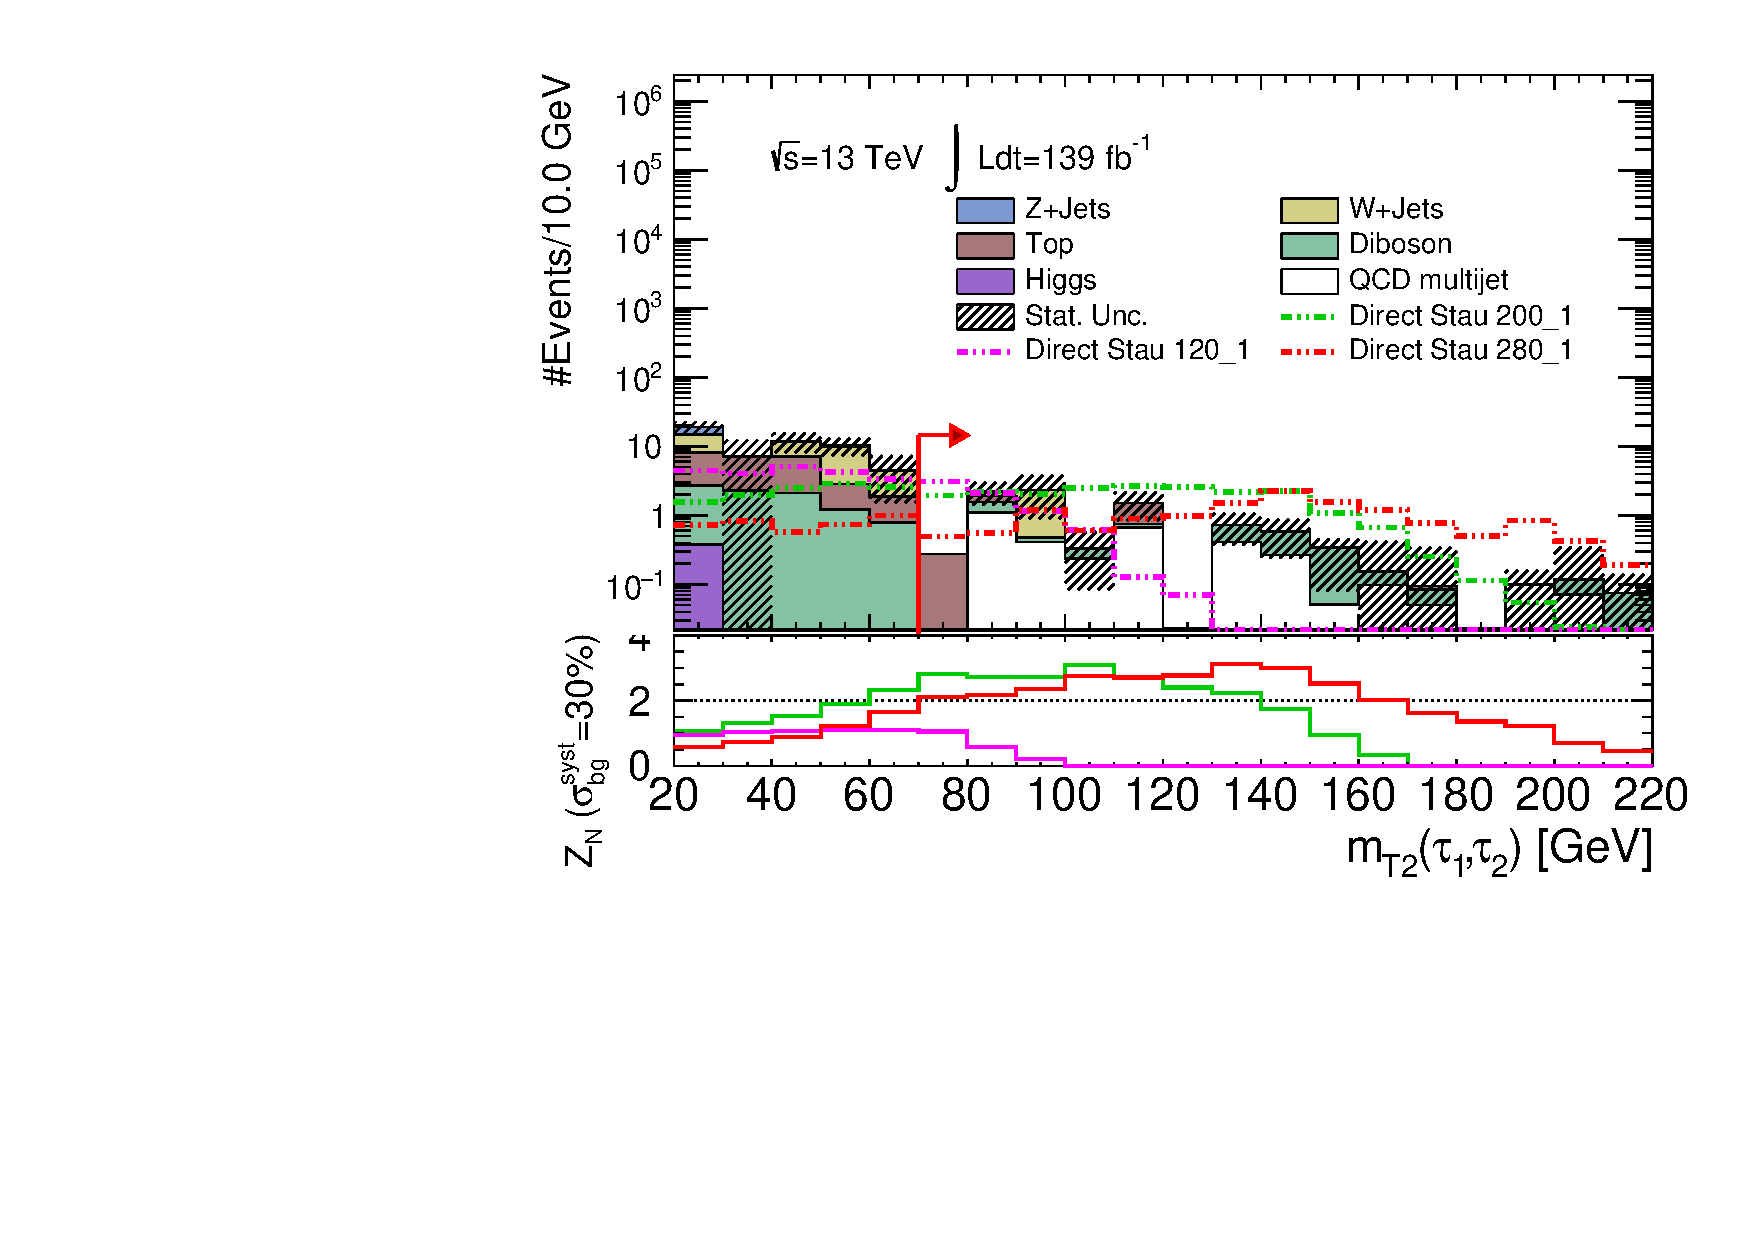
\includegraphics[width=0.4\textwidth]{Analysis/SRH/MT2_N_1}}\hspace{0.05\textwidth}	 
			 \subbottom[\met ($75\,<\,E_T^{miss}\,<\,150\,$ GeV)]{
				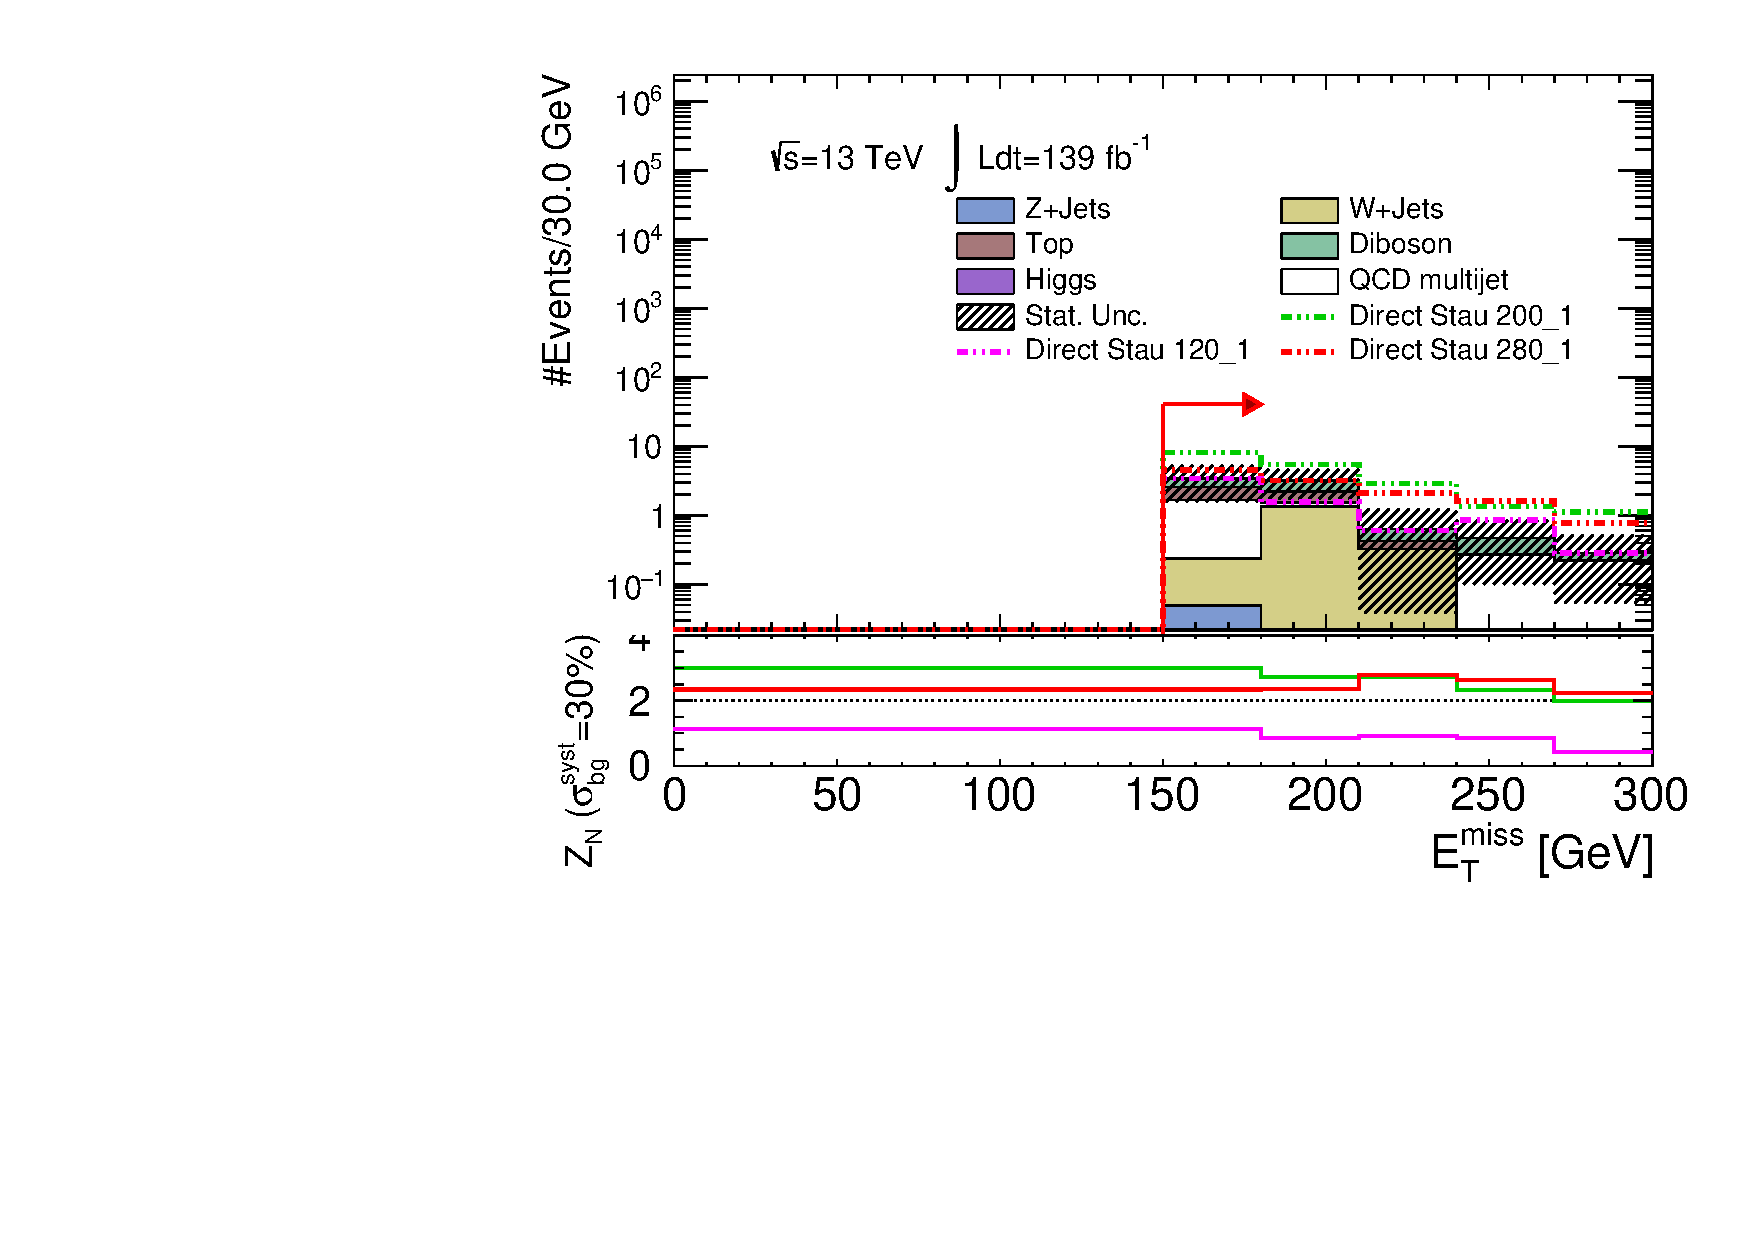
\includegraphics[width=0.4\textwidth]{Analysis/SRH/MET_N_1}}\hspace{0.05\textwidth}
			\subbottom[$\Delta R(\tau_1,\tau_2)$ ($\Delta R (\tau_1,\tau_2)\,<\,3.2$)]{
				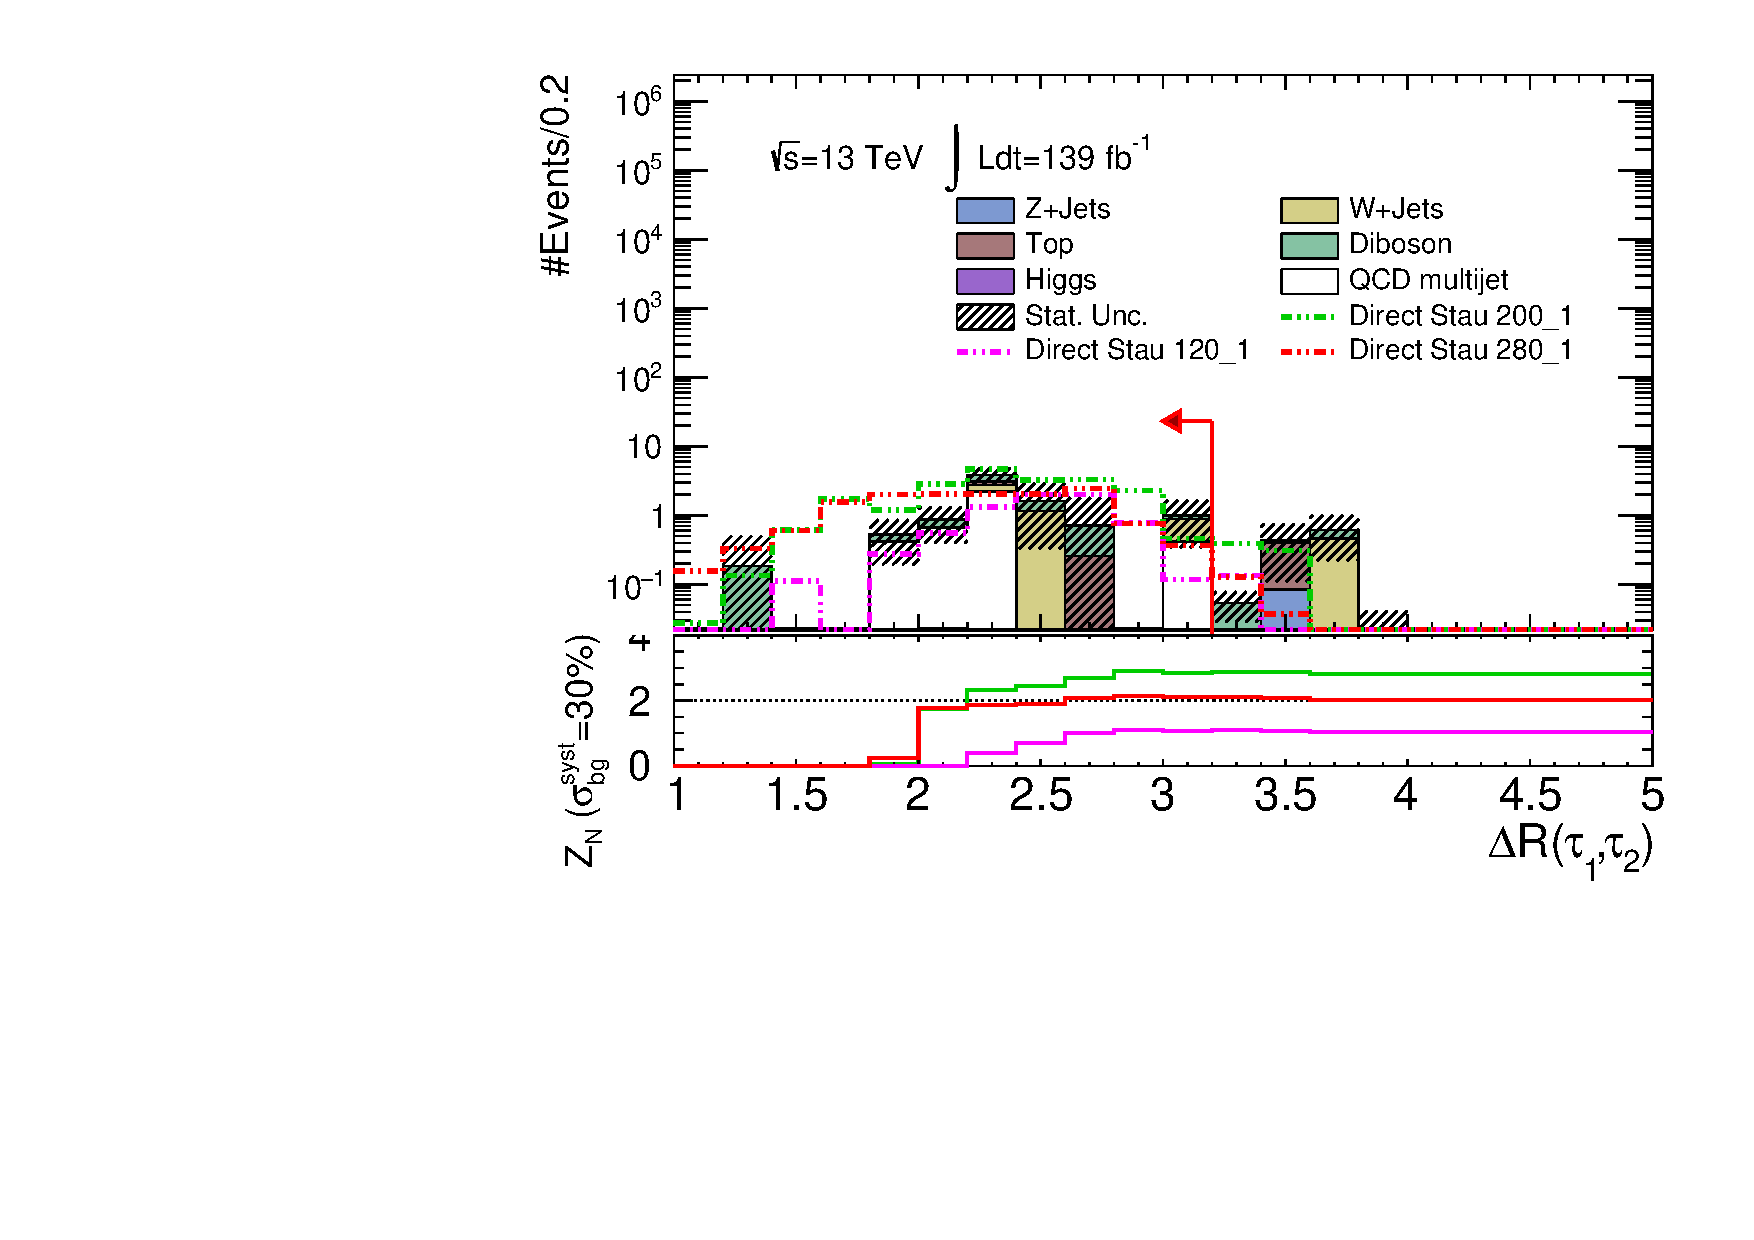
\includegraphics[width=0.4\textwidth]{Analysis/SRH/DR_N_1}}\hspace{0.05\textwidth}	 
			 \subbottom[$|\Delta\phi(\tau_1,\tau_2)|$ ($|\Delta\phi(\tau_1,\tau_2)|\,>\,0.8$)]{
				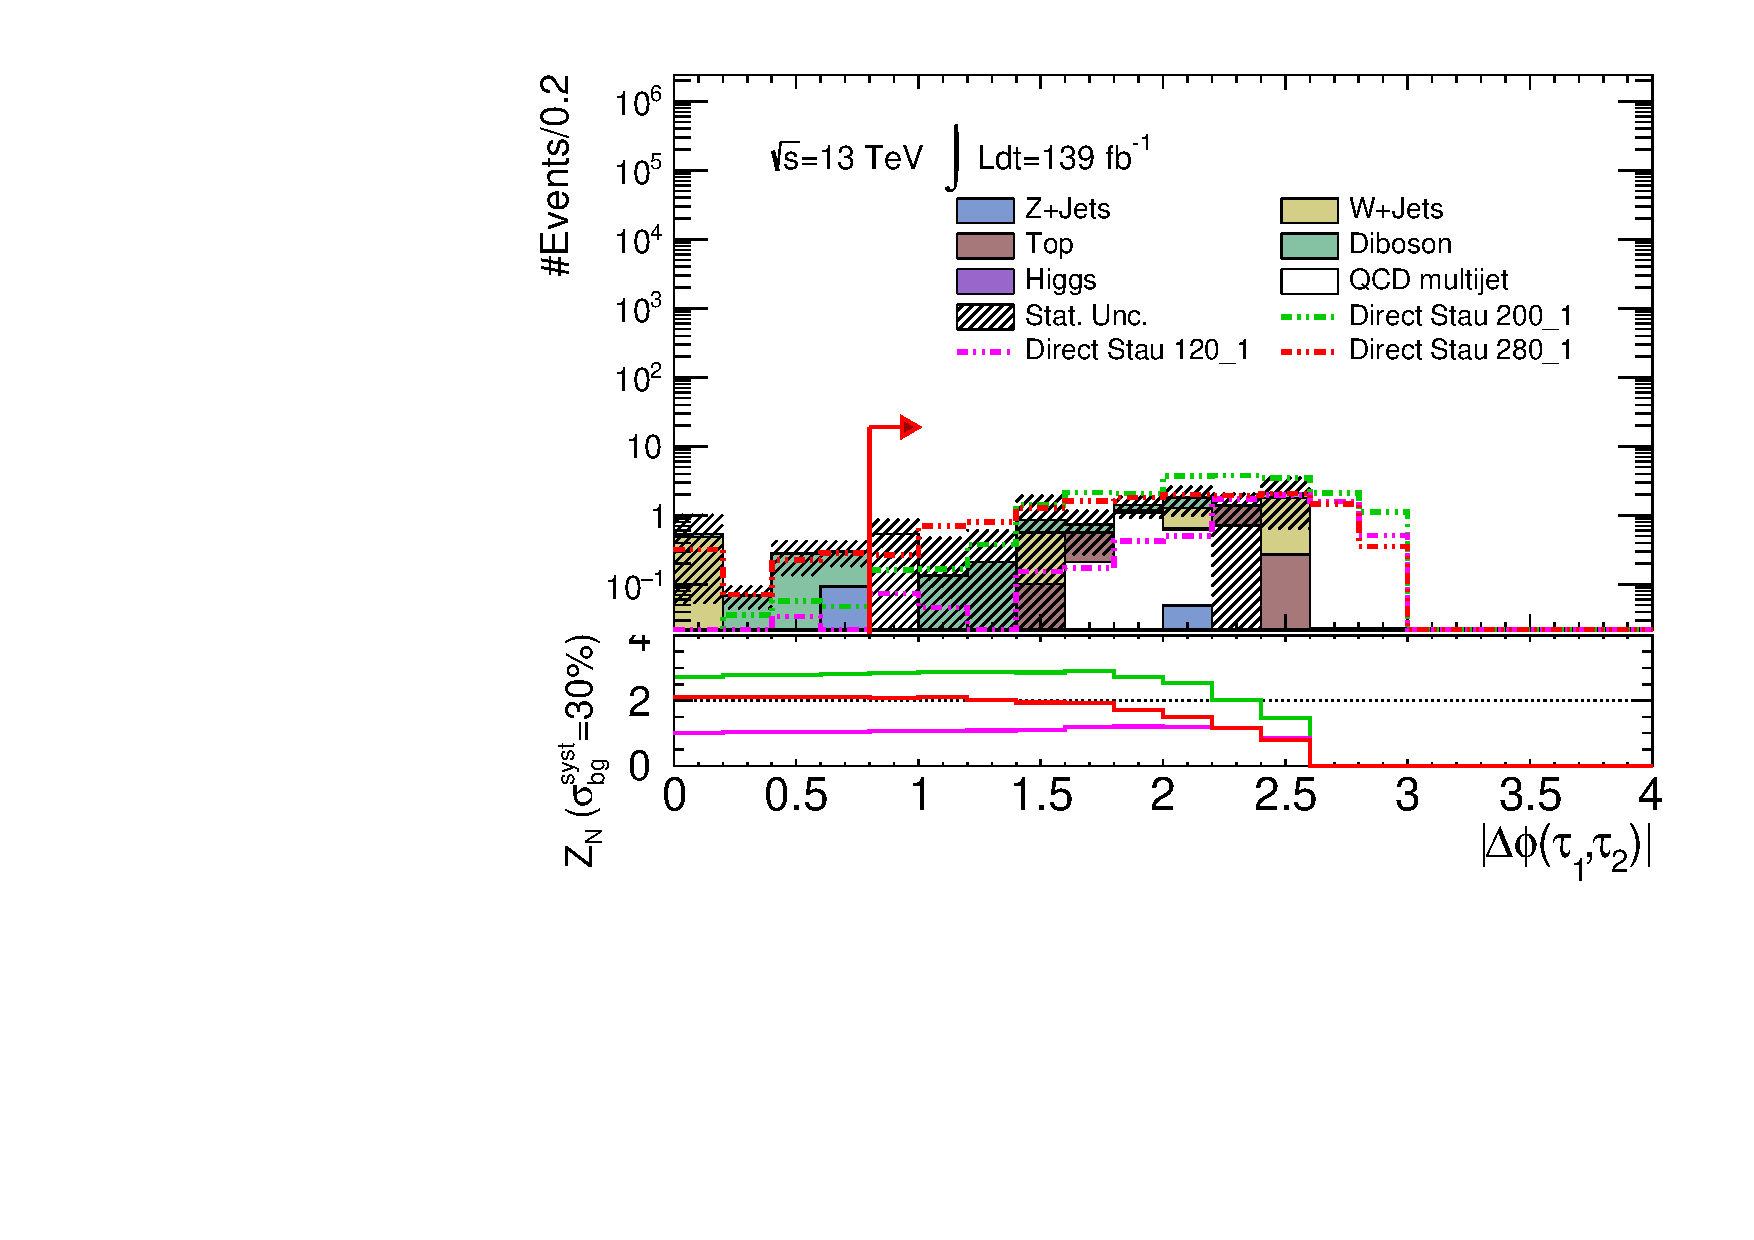
\includegraphics[width=0.4\textwidth]{Analysis/SRH/DPhi_N_1}}\hspace{0.05\textwidth}
		\end{center}
		\caption{"N-1" distributions of relevant kinematic variables after High-mass \ac{SR} requirements, except the one on the shown variable, are applied. The stacked histogram show the expected \ac{SM} background estimates from \ac{MC} normalised to 139 fb$^{-1}$.}
	\label{fig:SRH_analysis_N_1}
	\end{figure}	
	
	\subsection{Background estimation}
	\label{subsec:CRest}
	The main \ac{SM} backgrounds to this analysis are the multi-jet events, \Wjets, and multi-boson production, as explained in Section ~\ref{sec:smsamples}. Background events may contain a combination of "real" \ltau s or "fake" \ltau s. 
	The "real" \ltau s are defined as correctly identified prompt \htau s, while the "fake" \ltau s are which originate from a misidentified quark or gluon jet, en electron, or a muon.
	
	Multi-jet and \Wjets\ events are known as \textit{reducible} backgrounds. These are \ac{SM} processes whose final states involve either one or both final state objects to be mis-identified as \ltau s. 
	The contributions of the reducible background in the \acp{SR}  is thus estimated in data from dedicated \acp{CR}. 
	On the other hand the multi-boson, \Zjets, and \ttV ($V=W,Z$) background processes contribute mainly events containing real \ltau s, and are therefore called \textit{irreducible} backgrounds. To estimate the irreducible backgrounds, only \ac{MC} simulated samples are used and validated in dedicated \acp{VR}.
	\subsection*{Multi-jet background estimation}
	\label{subsec:ABCD_method}
	
	One of the dominant backgrounds in the \acp{SR} originates from jets mis-identified \ltau s in multi-jet production. It accounts for 44\% (30\%) of the total \ac{SM} contribution in the Low-mass (High-mass) \ac{SR}.
	This contribution is estimated using the so-called \textit{ABCD method}. 
	This method is an alternative to the \ac{FF} method described in detail in chapter~\ref{ch:fake_est}, which was not used in this analysis as it is not yet an \ac{ATLAS}-approved method.
	
	\ABCDschematics	
	Four exclusive regions, labelled as A, B, C  and D are defined in a two dimensional plane as a function of two (or more) uncorrelated discriminating variables. Regions A, B and C are dedicated \ac{CR} while region D is the \ac{SR}.  Figure ~\ref{fig:ABCD_schematics} shows the schematically drawn ABCD regions used in the analysis estimation of multi-jet  background.
	 The ratio of events in the regions C and B is then equal to that in the regions D and A.
	The number of multi-jet events in region D ($N_D$) can thus be calculated from the multi-jet events in region A ($N_A$) multiplied by the transfer factor $T=N_C/N_B$ where $N_C$ ($N_C$) is the number of multi-jet events in region C (B). Regions A, B, C, D are labelled as \ac{CR}-A, \ac{CR}-B, \ac{CR}-C, and Low-mass \ac{SR} (or  High-mass \ac{SR}), respectively. The ABCD method only provides a first-order estimate of multi-jet background, the normalised and uncertainty being then modified by a combined fit to \ac{CR}-A 	for both Low-mass and High-mass \ac{SR}. 
	The \ac{CR}-A and \ac{SR}-D are defined in the same way expect that the in the former the taus are required to pass the loose jet \ac{BDT} requirement but to fail the medium jet \ac{BDT} requirement to be orthogonal with \ac{SR}-D and reduce the signal contamination in \acp{CR}. The same tau \ac{BDT} identification criteria and charge requirements as in \ac{CR}-A (\ac{SR}-D) of the two taus is applied in \ac{CR}-B (\ac{CR}-C). In \ac{CR}-B and  \ac{CR}-C, less stringent requirements on the kinematic variables $M_{T2}$ and \met\ are applied. Furthermore, two validation regions, \ac{VR}-E and \ac{VR}-F are defined with similar definitions as  \ac{CR}-A and  \ac{SR}-D, respectively, except for intermediate requirements on the kinematic variables.The validation regions are used to verify the extrapolation of the ABCD estimation to the \ac{SR}-D, and to estimate the systematic uncertainty from the residual correlation between the tau-identification, the charge requirement, and kinematic variables. 
 	The definitions of the control and validations regions used are summarised in Table ~\ref{tab:ABCD_regions}, only for those requirements that are different in the \acp{CR},\acp{VR} with respect to the \acp{SR}. Requirements not listed in \acp{SR} definitions in Table~\ref{tab:ABCD_regions} but present in Table\ref{tab:analysis_SR} are applied to all ABCD method \acp{CR} and \acp{VR}. The \textit{asymmetric di-tau} (\textit{di-tau+\met}) triggers with corresponding scale factors are applied for Low-mass (High-mass) ABCD regions. 
	The number of multi-jet events in each control region and validation region is estimated from data after subtraction of other \ac{SM} contributions estimated from \ac{MC} simulation. 
	\begin{table}[!hbt]
	\centering
	\caption{The multi-jet \ac{CR} and \ac{VR} definitions for Low-mass (left) and High-mass (right) \acp{SR}. 
	Only requirements that different in the \acp{CR},\acp{VR} with respect to \ac{SR} definitions are listed.}
	\resizebox{\textwidth}{!}{
	%\documentclass[10pt]{article}
%\usepackage[usenames]{color} %used for font color
%\usepackage{amssymb} %maths
%\usepackage{amsmath} %maths
%\usepackage[utf8]{inputenc} %useful to type directly diacritic characters
%\begin{document}
%\begin{table}[]
%\resizebox{\textwidth}{!}{
\begin{tabular}{cc}
\hline
\multicolumn{2}{c}{\textbf{Low-Mass}} \\ \hline \hline
\multicolumn{1}{c|}{\textbf{CR-A}} & \textbf{Low-mass SR (D)} \\ \hline
\multicolumn{1}{c|}{$\geq2$ loose $\tau$s} & $==2$ tight $\tau$s \\
\multicolumn{1}{c|}{< 2 medium $\tau$s (OS)} & -- \\
\multicolumn{1}{c|}{$\Delta R(\tau_1,\tau_2) <3.2$} & $\Delta R(\tau_1,\tau_2) <3.2$ \\
\multicolumn{1}{c|}{$75<E_T^{miss}<150$ GeV} & $75<E_T^{miss}<150$ GeV \\
\multicolumn{1}{c|}{$M_{T2} > 70$ GeV} & $M_{T2} > 70$ GeV \\ \hline \hline
\multicolumn{1}{c|}{\textbf{VR-E}} & \textbf{VR-F} \\ \hline
\multicolumn{1}{c|}{$\geq2$ loose $\tau$s} & $==2$ tight $\tau$s (OS) \\
\multicolumn{1}{c|}{< 2 medium $\tau$s (OS)} & -- \\
\multicolumn{1}{c|}{$\Delta R(\tau_1,\tau_2) <3.2$} & $\Delta R(\tau_1,\tau_2) <3.2$ \\
\multicolumn{1}{c|}{$E_T^{miss}<150$ GeV} & $E_T^{miss}<150$ GeV \\
\multicolumn{1}{c|}{$30 < M_{T2} < 70$ GeV} & $30 < M_{T2} < 70$ GeV \\ \hline \hline
\multicolumn{1}{c|}{\textbf{CR-B}} & \textbf{CR-C} \\ \hline
\multicolumn{1}{c|}{$\geq2$ loose $\tau$s} & $==2$ tight $\tau$s (OS) \\
\multicolumn{1}{c|}{< 2 medium $\tau$s (OS)} & -- \\
\multicolumn{1}{c|}{no $\Delta R(\tau_1,\tau_2)$ cut} & no $\Delta R(\tau_1,\tau_2)$ cut \\
\multicolumn{1}{c|}{$E_T^{miss}<150$ GeV} & $E_T^{miss}<150$ GeV \\
\multicolumn{1}{c|}{$10 < M_{T2} < 30$ GeV} & $10 < M_{T2} < 30$ GeV \\ \hline 
\end{tabular}
%}

%\end{table}
%
%\end{document}	
	\quad
	%\documentclass[10pt]{article}
%\usepackage[usenames]{color} %used for font color
%\usepackage{amssymb} %maths
%\usepackage{amsmath} %maths
%\usepackage[utf8]{inputenc} %useful to type directly diacritic characters
%\begin{document}
%\begin{table}[]
%\resizebox{\textwidth}{!}{
\begin{tabular}{cc}
\hline
\multicolumn{2}{c}{\textbf{High-Mass}} \\ \hline \hline
\multicolumn{1}{c|}{\textbf{CR-A}} & \textbf{High-mass SR (D)} \\ \hline
\multicolumn{1}{c|}{$\geq2$ loose $\tau$s} & $==2$ medium $\tau$s \\
\multicolumn{1}{c|}{< 2 medium $\tau$s (OS)} & $\geq1$ tight $\tau$ \\
\multicolumn{1}{c|}{$\Delta R(\tau_1,\tau_2) <3.2$} & $\Delta R(\tau_1,\tau_2) <3.2$ \\
\multicolumn{1}{c|}{$E_T^{miss}>150$ GeV} & $E_T^{miss}>150$ GeV \\
\multicolumn{1}{c|}{$M_{T2} > 70$ GeV} & $M_{T2} > 70$ GeV \\ \hline \hline
\multicolumn{1}{c|}{\textbf{VR-E}} & \textbf{VR-F} \\ \hline
\multicolumn{1}{c|}{$\geq2$ loose $\tau$s} & $==2$ medium $\tau$s (OS) \\
\multicolumn{1}{c|}{< 2 medium $\tau$s (OS)} & $\geq1$ tight $\tau$ \\
\multicolumn{1}{c|}{$\Delta R(\tau_1,\tau_2) <3.2$} & $\Delta R(\tau_1,\tau_2) <3.2$ \\
\multicolumn{1}{c|}{$50<E_T^{miss}<100$ GeV} & $50<E_T^{miss}<100$ GeV \\
\multicolumn{1}{c|}{$50 < M_{T2} < 70$ GeV} & $50 < M_{T2} < 70$ GeV \\ \hline \hline
\multicolumn{1}{c|}{\textbf{CR-B}} & \textbf{CR-C} \\ \hline
\multicolumn{1}{c|}{$\geq2$ loose $\tau$s} & $==2$ medium $\tau$s (OS) \\
\multicolumn{1}{c|}{< 2 medium $\tau$s (OS)} & $\geq1$ tight $\tau$ \\
\multicolumn{1}{c|}{no $\Delta R(\tau_1,\tau_2)$ cut} & no $\Delta R(\tau_1,\tau_2)$ cut \\
\multicolumn{1}{c|}{$50<E_T^{miss}<100$ GeV} & $50<E_T^{miss}<100$ GeV \\
\multicolumn{1}{c|}{$30 < M_{T2} < 50$ GeV} & $30 < M_{T2} < 50$ GeV \\ \hline 
\end{tabular}

%}

%\end{table}
%
%\end{document}	
	}
	\label{tab:ABCD_regions}
	\end{table}
	The contribution from multijet events in the Low-mass (High-mass) \ac{CR}-B and \ac{VR}-E is around 96\% and 90\% (75\% and 79\%), respectively. The multi-jet impurity in \ac{CR}-A, \ac{CR}-C, and \ac{VR}-F is 74\%, 57\% and 51\% (58\%, 53\%, and 51\%), respectively, for Low-mass (High-mass) regions. 
	The signal contamination is defined as the ratio of number of signal events to the sum of signal and background events ($\textit{contamination}=N_{sig}/(N_{sig}+N_{bkg})$). The signal contamination in multi-jet \ac{CR}-A ranges from 0.4\% (1.2\%) to 9.4\% (21.4\%) for Low-mass (High-mass) \ac{SR}.
	
	The ABCD method is validated using a different method, the \textit{fake factor method}, which described in detail in Section~\ref{sec:ffmeth}. The predicted multi-jet event yields from the ABCD method and \ac{FF} method in both \acp{SR} and \acp{VR} agree within statistical and systematic uncertainties. 
	 
	\subsection*{W+jets background estimation}
	\label{subsec:Wjet_estimation}
	Around 25\% of the expects \ac{SM} background in the two \acp{SR} is expected to derive from the \Wjets\ production with at least one misidentified \ltau. A dedicated control region (WCR) is used to normalise the \Wjets\ \ac{MC} estimate to data and another region is then used to validate the estimate (WVR).
	The WCR is enriched in events where the W decays leptonically to a muon and a neutrino to suppress the contamination of multi-jet events.  Events for these regions are thus selected with a single-muon trigger. 
	Events are selected if they contain exactly one muon and one \ltau\ candidate of \ac{OS}. 
	The muon is required to have \pt\ > 50 \gev, while the \ltau\ candidate must satisfy the \textit{Medium} \ltau\ \ac{RNN} identification criteria and have \pt\ > 60 \gev. 
	 Top quark and \ttbar\ events are suppressed by rejecting events that contain $b$-tagged jets, or if they are compatible with \ttbar\ production (top-tagged)~\cite{Tovey_2008}. 
	 The transverse mass of the $\mu+$\met system ($m_{T,\mu}$) is used to reduce the contribution from \Zjets, top-quarks, and multi-boson events.
	  The \met\ and $\Delta R(\tau,\mu)$ cut are applied to further reduce the multi-jet and \Zjets\ contribution, while the invariant mass and sum of transverse mass of the muon and \ltau\ ($m(\tau,\mu)$ and $m_{T,mu}+m_{T,tau}$) are used to improve the \Wjets\ purity. Events in the WCR (WVR) are selected by requiring low (high) $m_{T2}$.
	  The selection applied in the WCR and WVR using the cuts described above is summarised in Table~\ref{tab:WCR_WVR}.
	\begin{table}[!hbt]
	\centering
	\caption{Summary of selection requirements for the \Wjets\ control (WCR) and validation (WVR) regions.}
	%\documentclass[10pt]{article}
%\usepackage[usenames]{color} %used for font color
%\usepackage{amssymb} %maths
%\usepackage{amsmath} %maths
%\usepackage[utf8]{inputenc} %useful to type directly diacritic characters
%\begin{document}
%\begin{table}[]
\begin{tabular}{cc}
\hline
WCR & WVR \\ \hline \hline
\multicolumn{2}{c}{1 medium $\tau$ and 1 isolated $\mu$ (OS)} \\
\multicolumn{2}{c}{single-muon trigger} \\
\multicolumn{2}{c}{$p_T(\tau)>60$ GeV,  $p_T(\mu)>50$ GeV} \\
\multicolumn{2}{c}{$E_T^{miss} > 60$ GeV} \\
\multicolumn{2}{c}{$b$-jet veto and top-tagged events veto} \\
\multicolumn{2}{c}{$m(\mu,\tau)>70$ GeV} \\
\multicolumn{2}{c}{$1<\Delta R(\mu,\tau)<3.5$} \\
\multicolumn{2}{c}{$50<m_{T,\mu}<150$ GeV} \\
\multicolumn{2}{c}{$m_{T,\mu}+m_{T,\tau}>250$ GeV} \\
\multicolumn{1}{c|}{$30<m_{T2}<70$ GeV} & $m_{T2}>70$ GeV \\ \hline
\end{tabular}
%\end{table}
%
%\end{document}	
	\label{tab:WCR_WVR}
	\end{table}
	
	The contribution of multi-jet events in the WCR (WVR) is estimated using the so-called \textit{OS-SS method}. The OS-SS method is performed by counting the number of events in data that satisfy the same requirements  as for the WCR (WVR) but with electric charge of the two leptons having the \ac{SS}. \ac{MC} processes other than multi-jet production are subtracted from the data counts in the \ac{SS} region using \ac{MC} simulation. This method relies on the fact that the ratio of \ac{SS} to \ac{OS} events in multi-jet events is close to unity while for \Wjets\ process is around 0.14.
	This is due to the latter process having events dominated by $gu/gd$-initiated processes that often give rise to a jet originating from the quark, which charge is anti-correlated with the $W$ boson charge. 
	The systematic uncertainty assigned to the multi-jet estimate in the WCR is 100\%, based on studies performed on simulated samples. 
	The prefit $m_{T2}$ distribution in the WCR is shown in Figure~\ref{fig:WCR}. Good agreement is observed both for the normalization and shape between data and \ac{SM} prediction, and the purity of the \Wjets selection is found to be around 79\%. The purity in the WVR is around 69\%. The contamination of signal  in WCR and WVR is negligible.
	\begin{figure}[!hbt]
		\centering
		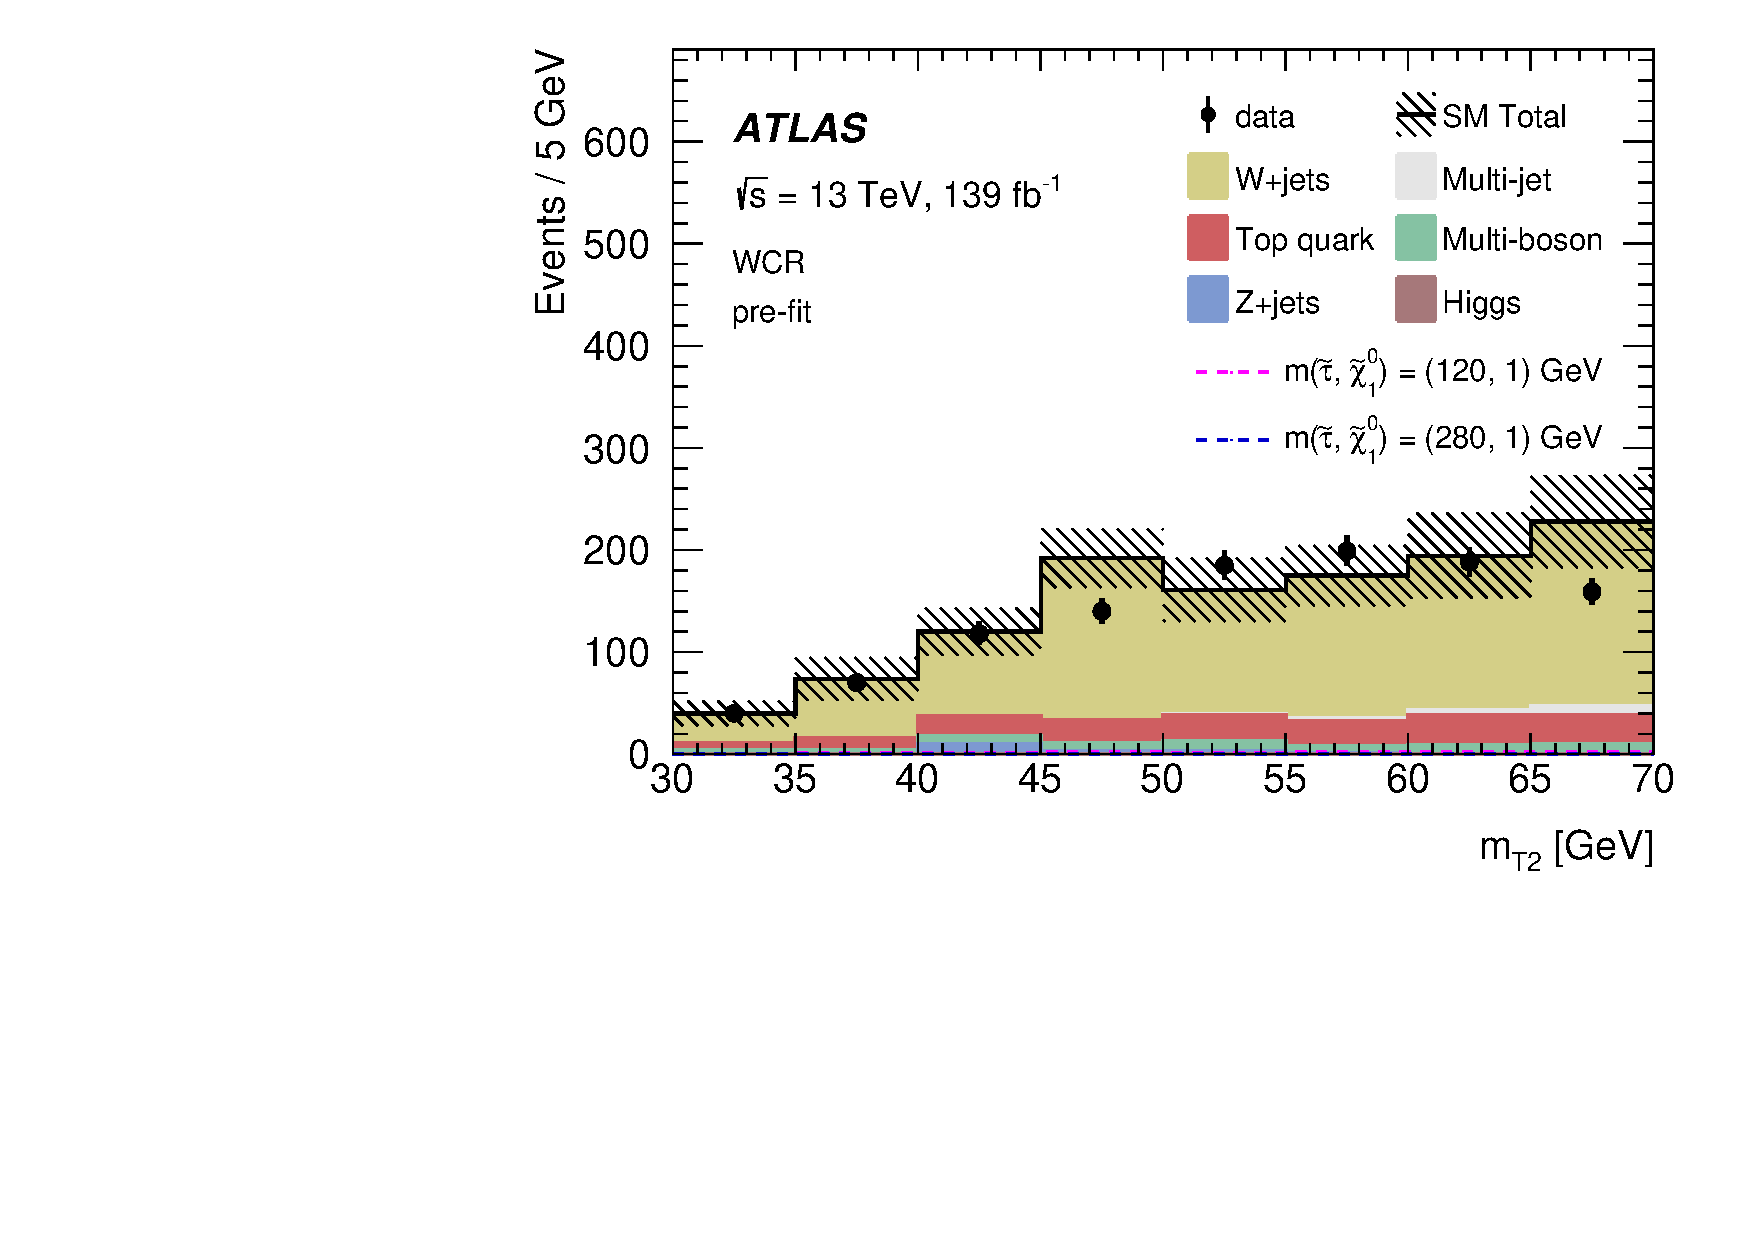
\includegraphics[width=0.75\textwidth]{Analysis/WCR/fig_04a}
		\caption{The prefit $M_{T2}$ distribution in the WCR. The \ac{SM} multi-jet production background is estimated from data using the OS-SS method, while all other backgrounds are estimated from  \ac{MC} simulation. Hatched bands represent the combined statistical and systematic uncertainties of the total \ac{SM} background. Distribution of \ac{SUSY} signal are shown but the contribution is too low to be visible. }
	\label{fig:WCR}
	\end{figure}	
	
	
	\subsection*{Irreducible background estimation}
	Irreducible \ac{SM} backgrounds arise mainly from \ttbar, single top quark, \ttV, \Zjets, and multiboson processes. All other \ac{SM} backgrounds are found to be negligible.  These relevant irreducible backgrounds are estimated with \ac{MC} simulations an validated in dedicated \acp{VR}, enriched with events from the process to be validated. 
	\begin{description}
	\item[Z+jets  Validation Refion (ZVR):] To suppress top-quark background, $b$-tagged events are vetoed. To enhance the purity of  \Zjets\ events, $\Delta R(\tau_1,\tau_2)$, $m(\tau_1,\tau_2)$, and $m_{T2}$ requirements are applied. 
	\item[Top Validation Refion (TVR):] To enrich the region with top-quark events a $\Delta R(\tau_1,\tau_2)$, requirement must be satisfied. There must also be at least on $b$-tagged jet with \pt\ > 20 \gev. An additional requirement on the $m_{T2} > 60$ \gev\ is need to be close to the \acp{SR}.
	\item[Multiboson  Validation Refion (VVVR):] The purity of multi-boson events is enhanced via $m(\tau_1,\tau_2)$ $m_{T,\tau_1}+m_{T,\tau_2}$, and $m_{T2}$ requirements. Top-quark background is also suppressed by rejecting events that have at least one $b$-tagged jet.
	\end{description}
	For all \acp{VR} events are also required to have at least two \ltau s that satisfy the \textit{Medium} \ac{RNN} identification criteria with opposite sign charge, and at least one \ltau\ candidate must satisfy the \textit{Tight} \ac{RNN} identification criteria, in order to be close to the \ac{SR}. 
	Events must also pass either the combined di-$\tau$+\met\ trigger or the asymmetric di-$\tau$ trigger for the High-mass and Low-mass selections, respectively.
	Table~\ref{tab:irreducible_VRs} gives a total summary of the described \acp{VR} selection criteria.
	\begin{table}[!hbt]
	\centering
	\caption{Summary of selection requirements for top quark (TVR), \Zjets\ (ZVR) and multiboson (VVVR) validation regions.}
	\resizebox{\textwidth}{!}{
	%\documentclass[10pt]{article}
%\usepackage[usenames]{color} %used for font color
%\usepackage{amssymb} %maths
%\usepackage{amsmath} %maths
%\usepackage[utf8]{inputenc} %useful to type directly diacritic characters
%\begin{document}
%\begin{table}[]
%\resizebox{\textwidth}{!}{
\begin{tabular}{ccc}
\hline
\multicolumn{3}{c}{\textbf{Low-Mass}} \\ \hline \hline
\textbf{TVR} & \textbf{ZVR} & \textbf{VVVR} \\ \hline
\multicolumn{3}{c}{$\geq2$ medium $\tau$ (OS), $\geq1$ tight $\tau$} \\
\multicolumn{1}{c|}{$\geq$1 $b$-jet} & \multicolumn{1}{c|}{$b$-jet veto} & $b$-jet veto \\
\multicolumn{1}{c|}{---} & \multicolumn{1}{c|}{$m(\tau_1,\tau_2)<70$ GeV} & $m(\tau_1,\tau_2)<110$ GeV \\
\multicolumn{1}{c|}{$\Delta R(\tau_1,\tau_2)>$1.2} & \multicolumn{1}{c|}{$\Delta R(\tau_1,\tau_2)<$1} & --- \\
\multicolumn{1}{c|}{---} & \multicolumn{1}{c|}{---} & $m_{T,\tau_1}+m_{T,\tau_2}>250$ GeV \\
\multicolumn{1}{c|}{$m_{T2} > $60 GeV} & \multicolumn{1}{c|}{$m_{T2} < $60 GeV} & $m_{T2} > $60 GeV \\
\multicolumn{3}{c}{asymmetric di-$\tau$ trigger} \\
\multicolumn{3}{c}{$60<E_T^{miss}<150$ GeV} \\
\multicolumn{3}{c}{$\tau_1$ and $\tau_2$ trigger $p_T$  requirements} \\ \hline
\end{tabular}
%}

%\end{table}
%
%\end{document}	
	\quad
	%\documentclass[10pt]{article}
%\usepackage[usenames]{color} %used for font color
%\usepackage{amssymb} %maths
%\usepackage{amsmath} %maths
%\usepackage[utf8]{inputenc} %useful to type directly diacritic characters
%\begin{document}
%\begin{table}[]
%\resizebox{\textwidth}{!}{
\begin{tabular}{ccc}
\hline
\multicolumn{3}{c}{\textbf{High-Mass}} \\ \hline
\textbf{TVR} & \textbf{ZVR} & \textbf{VVVR} \\ \hline
\multicolumn{3}{c}{$\geq2$ medium $\tau$ (OS), $\geq1$ tight $\tau$} \\
\multicolumn{1}{c|}{$\geq$1 $b$-jet} & \multicolumn{1}{c|}{$b$-jet veto} & $b$-jet veto \\
\multicolumn{1}{c|}{---} & \multicolumn{1}{c|}{$m(\tau_1,\tau_2)<60$ GeV} & $m(\tau_1,\tau_2)<110$ GeV \\
\multicolumn{1}{c|}{$\Delta R(\tau_1,\tau_2)>$1.2} & \multicolumn{1}{c|}{$\Delta R(\tau_1,\tau_2)<$1} & --- \\
\multicolumn{1}{c|}{---} & \multicolumn{1}{c|}{---} & $m_{T,\tau_1}+m_{T,\tau_2}>200$ GeV \\
\multicolumn{1}{c|}{$m_{T2} > $60 GeV} & \multicolumn{1}{c|}{$m_{T2} < $60 GeV} & $m_{T2} > $60 GeV \\
\multicolumn{3}{c}{di-$\tau+E_T^{miss}$ trigger} \\
\multicolumn{3}{c}{$E_T^{miss}>150$ GeV} \\
\multicolumn{3}{c}{$\tau_1$ and $\tau_2$ trigger $p_T$  requirements} \\ \hline
\end{tabular}
%}

%\end{table}
%
%\end{document}	
	}
	\label{tab:irreducible_VRs}
	\end{table}
	The data event yields and the SM predictions in the WVR,  TVR, and VVVR are shown in Figure~\ref{fig:irreducible_VRs}. The data and \ac{SM} prediction in each validation region agree within the uncertainties. 
	The purity of the selection in \Zjets\, \ttbar and multiboson events are 83\%-96\%, 83\%-96\%, and 47\%-71\% in the respective validation regions. 
	\begin{figure}[!hbt]
		\centering
		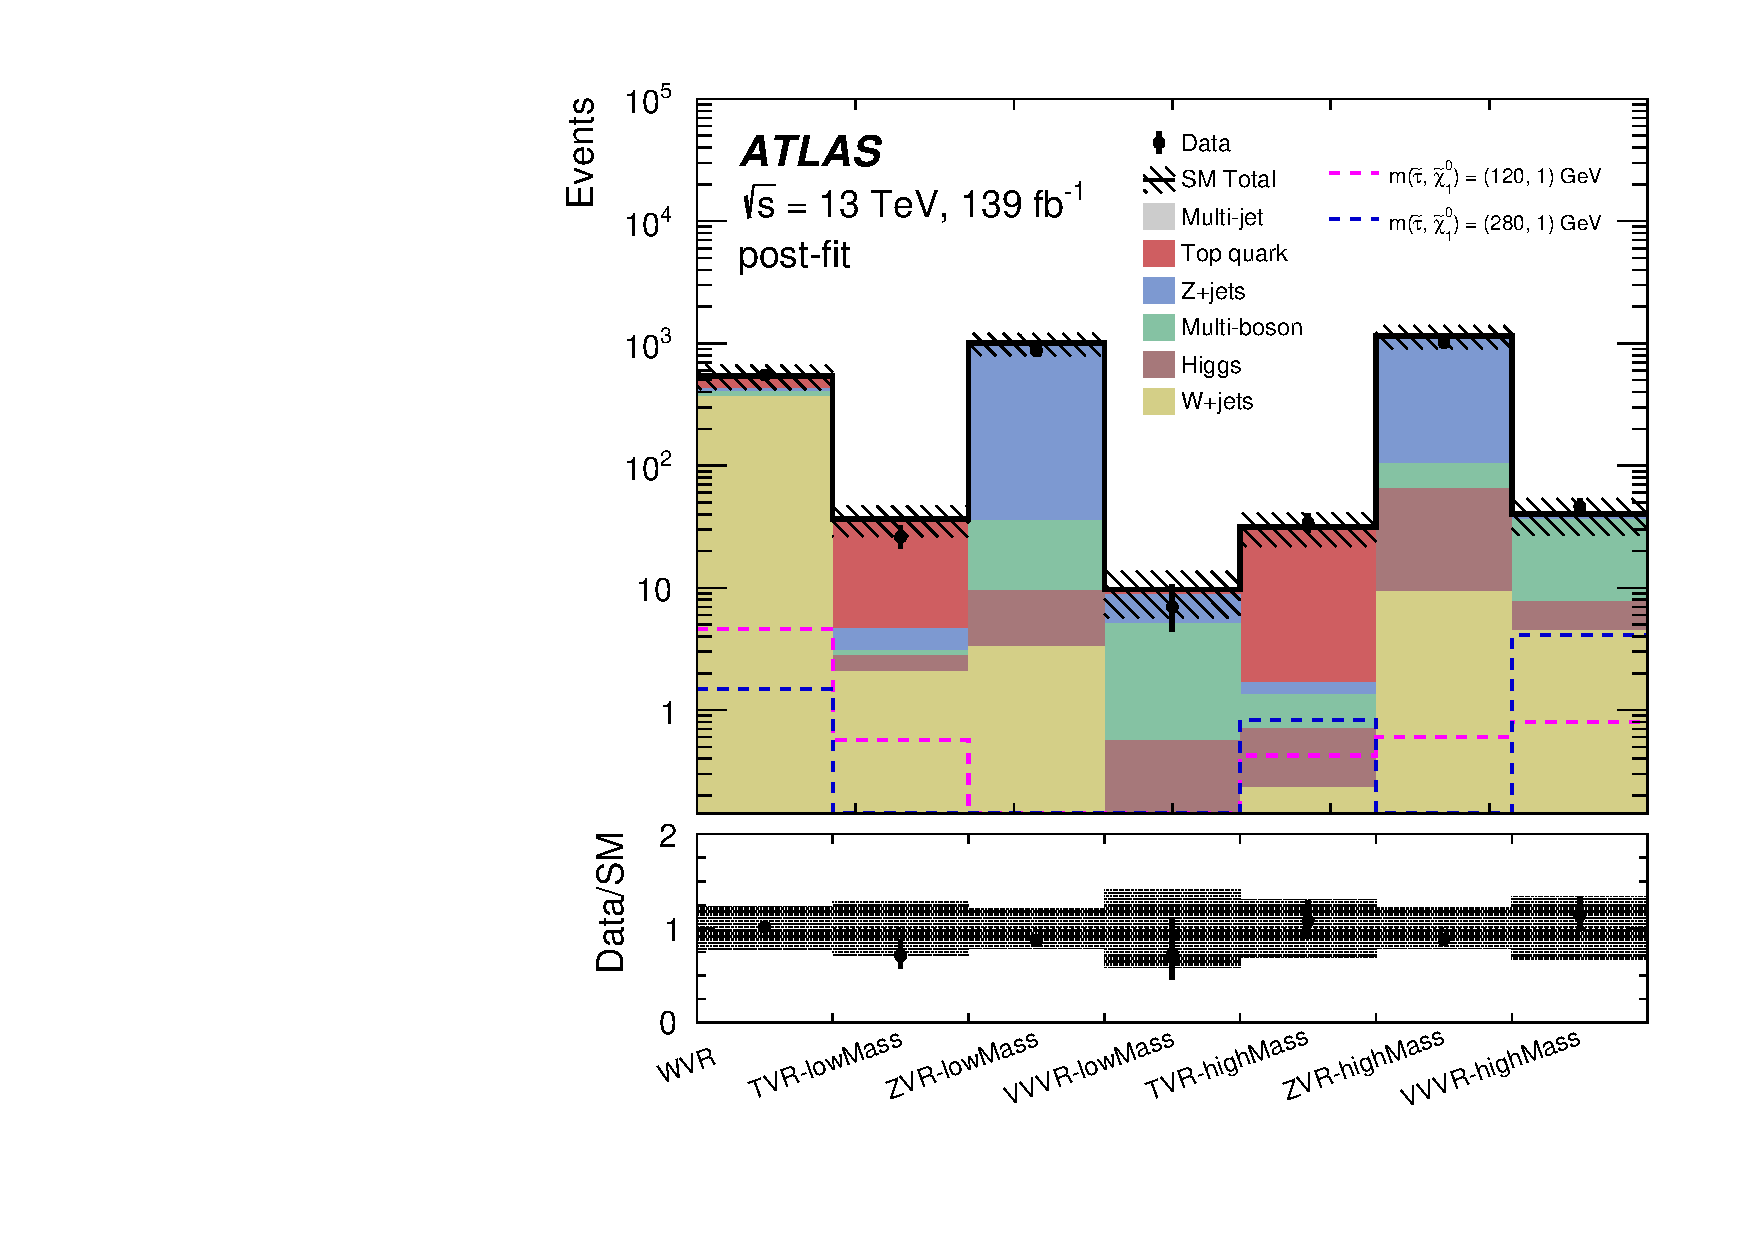
\includegraphics[width=0.75\textwidth]{Analysis/Irreducible/fig_05}
		\caption{The postfit yields in the WVRs, TVRs, ZVRs  and VVVRs for both High-mass and Low-mass selections. The \ac{SM} multi-jet production background contribution is negligible and estimated from data using the OS-SS method, while all other backgrounds are estimated from  \ac{MC} simulation. Hatched bands represent the combined statistical and systematic uncertainties of the total \ac{SM} background. Distribution of \ac{SUSY} signal are also shown. The lower panel shows the ratio of data to the \ac{SM} background estimate.}
	\label{fig:irreducible_VRs}
	\end{figure}	
	
	\section{Systematic uncertainties}
	\label{sec:syst_unc}
	For this analysis several sources of systematic uncertainties are considered. These include: experimental uncertainties, which derive from the reconstruction of physics objects and the integrated luminosity of the analysed dataset used, as well as theoretical uncertainties on the modelling of the relevant \ac{SM} background and \ac{SUSY} signal processes.  
	
	The systematic uncertainties discussed here affect the predicted background yields in the \acp{SR} and are either used when evaluating a given background yield in the \acp{SR}, by relying on the sole \ac{MC} prediction, or when computing the uncertainty on the \ac{TF}.
	The overview of the sources of systematic uncertainties is presented in this thesis in two separate section. 
	One section will be dedicated to the experimental uncertainties that affect this analysis, while the other will describe the study and derivation of the theory uncertainties, that include uncertainties on cross sections, choice of scales, and \acp{PDF}, which was primarily performed by the author. 
	\subsection{Experimental uncertainties}
	Each reconstructed object has an assigned uncertainty. Dedicated calibrations of each physics objects ($e$, $\mu$, \htau, $b-$jets, and \met) are used to estimate the associated uncertainties. These calibrations are then added to the \ac{MC} samples as \eg\ lepton/photon reconstruction efficiencies, \ac{JES}, \ac{JER}, $b$-tagging efficiencies, \met\ reconstruction, etc. 
	A list of such non-negligible uncertainties for this analysis is given here:
	\begin{description}
	\item[\ac{JES} and \ac{JER}:] the \ac{JES} and \ac{JER} arise from the measured momentum of jets, which need to be calibrated to the right energy scale ~\cite{ATLAS13TeVJES}. 
	The uncertainty on the \ac{JES} is \pt\ and pseudorapidity ($\eta$) dependent, and is evaluated in \ac{MC} simulation using a set of grouped variations consisting of six \acp{NP}, which describe how the observed property is affected by the uncertainties.  
	 %Three $\eta$ intercalibration non-closure uncertainties each as a single \ac{NP}, and three additional \acp{NP} which are a combination of all the remaining parameters ($\mathcal{O}(100)$). 
	 Three $\eta$ intercalibration non-closure uncertainties and three additional uncertainties, the combination of all the remaining parameters ($\mathcal{O}(100)$), are used as a \ac{NP} each, for a total of six \acp{NP}.
	The uncertainty due to the \ac{JER} is evaluated by smearing the jet energy using a simple set of systematic variations with 8 \acp{NP}.
	\item[Hadronically decaying taus:] \ltau\ energy scale~\cite{Mitani:2199788}, resolution, and identification are one of the main sources of experimental systematic uncertainties in the \acp{SR}, because of the requirement of at least two of these objects to be present in the final selection. 
	 Uncertainties on the \ltau\ \ac{JES} are evaluated using \acp{SF} and corresponding uncertainties on the efficiency of reconstructing a jet, identifying it as a tau jet, and for passing the electron \ac{OR}.
	\item[Light leptons:] lepton reconstruction, identification and isolation efficiencies have contributions to the background. For electrons, uncertainties on the electron energy scale and resolution are evaluated by scaling and smearing the energies of electrons in simulated events. Similarly, muon uncertainties originating from the muon energy resolution, isolation, reconstruction and momentum scale are evaluated by modifying the energies of muons in simulated events. 		
	\item[\textit{b}-Jets:] \ac{SF} uncertainties in $b$-tagging depend on the kinematics of the jet and on the jet flavour. The efficiency of correctly identifying a jet originating from a $b$-quark, as well as the efficiency of incorrectly tagging a jet originating from a $c$ or light quark are modelled using three uncertainty variations to the $b$-jet weight called \textit{nominal}, \textit{up}, and \textit{down}, which are propagated to the \acp{SF} for $b$-jets.
	\item[\boldmath \met:] uncertainties on the missing transverse momentum are evaluated by propagating the uncertainties of the constituent objects, as described above. There is a residual uncertainty due to the "soft-term", which sums up the tracks not associated to any of the physics objects described above. Scale and resolution uncertainties for this term are evaluated by modifying it accordingly, and evaluating the effect of this change on the event selection. 
	\item[Pile-up:] the uncertainty on  the distribution of the number of simultaneous interactions in each $pp$ collision is performed by varying \mubar\ by $\pm4\%$. and using the modified parameter to perform a pile-up re-weighting procedure to match the distributions of the number of reconstructed bertices observed in data~\cite{PhysRevLett.117.182002}.
	\item[Trigger:] \ltau\ trigger \acp{SF} are a source of uncertainty that is implemented using results taken from dedicated measurements~\cite{ATLAS-CONF-2017-061} and are included with the \ltau\ identification uncertainty.
	\item[Luminosity:] an uncertainty in the integrated luminosity of $\pm2.0\%$ is applied for the combined 2015,2016, 2017, and 2018 dataset~\cite{ATLAS-CONF-2019-021}.
	
	The sources of uncertainties associated to the determination of the multijet background via the ABCD method are: the correlation among the \ltau\ identification, the charge requirement, and the kinematic variable $m_{T2}$, the limited number of events in the \acp{CR}, and the subtraction of the other \ac{SM} backgrounds.
	The systematic uncertainty in the correlation is determined by comparing the transfer factor described in section ~\ref{subsec:ABCD_method}, between \ac{CR}-B to \ac{CR}-C to that of \ac{VR}-E to \ac{VR}-F.   
	
	\begin{table}[!hbt]
	\centering
	\caption{The postfit relative systematic uncertainty (\%) in the  background estimate (signal reference points) in the Low-mass and High-mass \acp{SR} from the leading sources at top (bottom). Uncertainties from different sources in the background estimates may be correlated, and do not necessarily add in quadrature to the total uncertainty. }
	\resizebox{0.7\textwidth}{!}{
	%\documentclass[10pt]{article}
%\usepackage[usenames]{color} %used for font color
%\usepackage{amssymb} %maths
%\usepackage{amsmath} %maths
%\usepackage[utf8]{inputenc} %useful to type directly diacritic characters
%\begin{document}
%\begin{table}[]
\begin{tabular}{lcc}
\hline
\begin{tabular}[c]{@{}l@{}}Source of systematic uncertainty\\ on background prediction\end{tabular} & \begin{tabular}[c]{@{}c@{}}Low-mass SR\\ {[}\%{]}\end{tabular} & \begin{tabular}[c]{@{}c@{}}High-mass SR\\ {[}\%{]}\end{tabular} \\ \hline \hline
\begin{tabular}[c]{@{}l@{}}Statistical uncertainty \\ of MC samples\end{tabular} & 11 & 21 \\
\begin{tabular}[c]{@{}l@{}}$\tau$-lepton identification \\ and energy scale\end{tabular} & 19 & 10 \\
\begin{tabular}[c]{@{}l@{}}Normalization uncertainties \\ of multijet background\end{tabular} & 12 & 8 \\
Multijet estimation & 4 & 10 \\
Jet energy scale and resolution & 5 & 8 \\
\begin{tabular}[c]{@{}l@{}}$E_T^{miss}$ soft-term \\ resolution and scale\end{tabular} & 2 & 2 \\ 
\end{tabular}
%\end{table}
%
%\end{document}	}
	\resizebox{0.7\textwidth}{!}{
	%\documentclass[10pt]{article}
%\usepackage[usenames]{color} %used for font color
%\usepackage{amssymb} %maths
%\usepackage{amsmath} %maths
%\usepackage[utf8]{inputenc} %useful to type directly diacritic characters
%\begin{document}
%\begin{table}[]
\begin{tabular}{lcc}
\hline
\begin{tabular}[c]{@{}l@{}}Source of systematic uncertainty \\ on signal prediction\end{tabular} & \begin{tabular}[c]{@{}c@{}}Low-mass SR\\ {[}\%{]}\end{tabular} & \begin{tabular}[c]{@{}c@{}}High-mass SR\\ {[}\%{]}\end{tabular} \\ \hline \hline
$m(\tilde{\tau},\tilde{\chi}_1^0)$ {[}GeV{]} & (120,1) & (280,1) \\ \hline \hline
\begin{tabular}[c]{@{}l@{}}$\tau$-lepton identification \\ and energy scale\end{tabular} & 29 & 14 \\
\begin{tabular}[c]{@{}l@{}}Statistical uncertainty \\ of MC samples\end{tabular} & 6 & 10 \\
Jet energy scale and resolution & 3 & 2 \\
\begin{tabular}[c]{@{}l@{}}$E_T^{miss}$ soft-term \\ resolution and scale\end{tabular} & 3 & \textless{}1 \\ \hline
\end{tabular}
%\end{table}
%
%\end{document}	}
	\label{tab:exp_unc}
	\end{table}
	Table ~\ref{tab:exp_unc} summarises the main sources of experimental systematic uncertainties in the \ac{SM} background estimates for the Low-mass and High-mass \acp{SR}, where 
	the statistical uncertainty of the event yields in the \acp{CR} is propagated to the \acp{SR} as a systematic uncertainty.
	The dominant uncertainties in the \acp{SR} are the statistical uncertainty of the \ac{MC} prediction (11\%-21\%), \ltau\ identification and energy scale (10\%-19\%), and multijet background normalization (8\%-12\%).
	The total uncertainty in the signal yields for for the \ac{SUSY} reference points is about 17\%-31\% and are dominated by the \ltau\ identification and energy scale (14\%-29\%) and the statistical uncertainty of the signal \ac{MC} predictions (6\%-20\%).
	
	
	
	\end{description}
	\subsection{Theory Uncertainties}
	The theoretical uncertainties are evaluated by considering variations with respect to the nominal settings and choices for the event generation.
	The three main sources of theoretical uncertainties considered for this analysis are: the uncertainty associated to missing higher order corrections to the cross-section, the uncertainty on \acp{PDF}, and the uncertainty on the strong coupling ($\alpha_S$).
	The \textit{re-normalization scale} ($\mu_R$) give the dependence for the running strong coupling constant ($\alpha_S$), and is set to equal the momentum transfer $Q$ of the scattering. 
	The \textit{factorization scale} ($\mu_F$) refers to the separation of the hard scattering \ac{QCD} effects from the \ac{PDF}. 
	A \textit{scale variation}, \ie\ a variation of the re-normalisation and factorisation scales by some fixed factors, is generally used to estimate the uncertainty associated to the missing higher order in the perturbative expansion of the partonic cross-section.
	%The chosen scale also affects the cross-section calculation of the process. 
	The uncertainty on the \acp{PDF} will change accordingly to experimental uncertainties introduced in the datasets used in the \ac{PDF} fits. Two sets of \acp{PDF} are compared to the nominal \ac{PDF} to check the spread between the different \ac{PDF} sets and their uncertainties.  
	The strong coupling constant is determined experimentally from the combination of different datasets and its value is quoted at the scale of the $Z$ boson mass. The associated uncertainties are thus a combination of the experimental errors and the truncation of the theoretical value at a fixed order in perturbation theory.  
	 %The three main theoretical uncertainties thus considered are: the uncertainty associated to missing higher order corrections, the uncertainty on \acp{PDF}, and the uncertainty on the strong coupling ($\alpha_S$).%constant used for the generation of the \ac{MC} samples.
	 
	Each systematic uncertainty $i$ is described as a \ac{NP} ($\theta_i$) that parametrizes the impact on the parameter(s) of interest (\ie\ rate of signal process, normalization factors, etc.). They are thus described as variations from the nominal, \eg\ $\theta_i=\pm1$ for $\pm1\sigma$, where $1\sigma$ means one standard deviation.
	 
	The recipes used for the estimation of the theoretical uncertainties for the main backgrounds is below. 
	\begin{description}
	\item[Multiboson:] The prescription used for the estimation of the uncertainties for the higher order corrections requires the usage of the factorization and re-normalization scale variations. These implemented as seven weights in the nominal sample corresponding to the variations of the \ac{QCD} factorization and re-nomalization scales in the matrix element by a factor of 2 and 0.5,  avoiding variations in the opposite direction~\cite{QCDvar}. These uncertainties are then combined by taking the envelope of all the uncertainties. 
	Uncertainties on the \ac{PDF}+$\alpha_s$ are computed following the \textsc{PDF4LHC} prescriptions, that can be found in Ref.~\cite{PDF4LHC}, and include 100 variations as well as variations in the central value of the \ac{PDF}. A global 6\% uncertainty due to scale and \ac{PDF} should be applied to $WW/WZ/ZZ$ cross sections. 
	
	\item[\boldmath \ttbar, single top:] Uncertainties associated to the parton shower, which affect the event yield of the \ttbar\ background, are evaluated by comparing the predictions of \textsc{PowHeg+Pythia8} and \textsc{PowHeg+Herwig7}. The uncertainty associated to the \ac{ISR}/\ac{FSR} are also evaluated by comparing the predictions of \textsc{PowHeg+Pythia8} with two samples with varied radiation settings. These uncertainties are implemented as a \ac{NP} for each scale variation and process; they are not constraint.
	The inclusive cross section uncertainty at \ac{NNLO+NNLL} is 6\%.
	
	\item[\boldmath $W$,\boldmath$Z+$\textbf{jets}:] Similarly to the multi boson case, $W$/\Zjets\ modelling include uncertainties from the factorization and re-normalization scales, computed using different variations implemented as weights in the nominal sample. Uncertainties affecting the \textsc{Sherpa} event generator predictions are also estimated using the \ac{PDF} sets following the \textsc{PDF4LHC} recommendations.
	
	\item[SUSY signal:] signal cross sections are calculated at \ac{NLO + NLL} using the resummino code from Ref.~\cite{cite-1} with two sets of \acp{PDF} (\textsc{CTEQ6.6} and \textsc{MSTW2008nlo90cl}). Only the cross-section uncertainty is taken into account for signal processes and it varies from 2 to 3\% for the considered \ac{SUSY} models. 
	
	\begin{table}[!hbt]
	\centering
	\caption{Fractional variations from nominal of theoretical uncertainties in Low-mass \ac{SR} and High-mass \ac{SR}.
	%The the higher order cross-section via combination of re-normalisation and factorization scales, the strong coupling constant ($\alpha_s$), and the \acp{PDF}.
	}
	\resizebox{\textwidth}{!}{
	%\documentclass[10pt]{article}
%\usepackage[usenames]{color} %used for font color
%\usepackage{amssymb} %maths
%\usepackage{amsmath} %maths
%\usepackage[utf8]{inputenc} %useful to type directly diacritic characters
%\begin{document}
%\begin{table}[]
\begin{tabular}{lcccccc}
\cline{2-7}
 & \multicolumn{6}{c}{Low-mass SR} \\ \cline{2-7} \cline{2-7} 
 & \begin{tabular}[c]{@{}c@{}}Combined \{$\mu_R$,$\mu_F$\}\\ up / down\end{tabular} & \begin{tabular}[c]{@{}c@{}}$\mu_R$\\ up / down\end{tabular} & \begin{tabular}[c]{@{}c@{}}$\mu_F$\\ up / down\end{tabular} & \begin{tabular}[c]{@{}c@{}}$\alpha_S$\\ up / down\end{tabular} & \begin{tabular}[c]{@{}c@{}}PDF\\ up / down\end{tabular} & \begin{tabular}[c]{@{}c@{}}alt. PDF\\ up / down\end{tabular} \\ \hline \hline
\multirow{2}{*}{Higgs} & 0.193 & 0.103 & 0.027 & 0.091 & 0.017 & 0.016 \\
 & 0.116 & 0.115 & 0.037 & 0.036 & 0.013 & 0.012 \\ \hline
\multirow{2}{*}{Multiboson} & 0.248 & 0.237 & 0.010 & 0.026 & 0.020 & 0.018 \\
 & 0.168 & 0.161 & 0.006 & 0.044 & 0.020 & 0.001 \\ \hline
\multirow{2}{*}{Top} & 0.126 & 0.084 & 0.065 & 0.047 & 0.025 & 0.024 \\
 & 0.125 & 0.076 & 0.055 & 0.039 & 0.031 & 0.030 \\ \hline
\multirow{2}{*}{W+jets} & 0.355 & 0.353 & 0.012 & 0.038 & 0.023 & 0.015 \\
 & 0.221 & 0.219 & 0.011 & 0.049 & 0.026 & 0.008 \\ \hline
\multirow{2}{*}{Z+jets} & 0.362 & 0.359 & 0.009 & 0.061 & 0.027 & 0.005 \\
 & 0.232 & 0.229 & 0.009 & 0.067 & 0.031 & 0.001 \\ \hline
\end{tabular}
%\end{table}
%
%\end{document}	}
	\resizebox{\textwidth}{!}{
	%\documentclass[10pt]{article}
%\usepackage[usenames]{color} %used for font color
%\usepackage{amssymb} %maths
%\usepackage{amsmath} %maths
%\usepackage[utf8]{inputenc} %useful to type directly diacritic characters
%\begin{document}
%\begin{table}[]
\begin{tabular}{lcccccc}
\cline{2-7}
 & \multicolumn{6}{c}{High-mass SR} \\ \cline{2-7} \cline{2-7} 
 & \begin{tabular}[c]{@{}c@{}}Combined \{$\mu_R$,$\mu_F$\}\\ up / down\end{tabular} & \begin{tabular}[c]{@{}c@{}}$\mu_R$\\ up / down\end{tabular} & \begin{tabular}[c]{@{}c@{}}$\mu_F$\\ up / down\end{tabular} & \begin{tabular}[c]{@{}c@{}}$\alpha_S$\\ up / down\end{tabular} & \begin{tabular}[c]{@{}c@{}}PDF\\ up / down\end{tabular} & \begin{tabular}[c]{@{}c@{}}alt. PDF\\ up / down\end{tabular} \\ \hline \hline
\multirow{2}{*}{Higgs} & 0.134 & 0.093 & 0.017 & 0.056 & 0.015 & 0.014 \\
 & 0.099 & 0.101 & 0.013 & 0.018 & 0.011 & 0.010 \\ \hline
\multirow{2}{*}{Multiboson} & 0.270 & 0.257 & 0.014 & 0.037 & 0.022 & 0.016 \\
 & 0.195 & 0.183 & 0.013 & 0.070 & 0.023 & 0.000 \\ \hline
\multirow{2}{*}{Top} & 0.152 & 0.113 & 0.039 & 0.045 & 0.062 & 0.027 \\
 & 0.142 & 0.075 & 0.043 & 0.033 & 0.030 & 0.029 \\ \hline
\multirow{2}{*}{Wjets} & 0.411 & 0.396 & 0.014 & 0.128 & 0.031 & 0.006 \\
 & 0.256 & 0.246 & 0.012 & 0.094 & 0.030 & 0.012 \\ \hline
\multirow{2}{*}{Zjets} & 0.391 & 0.375 & 0.016 & 0.058 & 0.031 & 0.011 \\
 & 0.246 & 0.233 & 0.013 & 0.053 & 0.028 & 0.002 \\ \hline
\end{tabular}

%\end{table}
%
%\end{document}	}
	\label{tab:theo_unc_SR}
	\end{table}
	The theoretical uncertainties determined for the Low-mass and High-mass \acp{SR} for the most relevant \ac{SM} backgrounds are shown in Table~\ref{tab:theo_unc_SR}.
	The uncertainties are shown as fractional values for the \textit{up} and \textit{down} variations from the nominal value of interest.
	The uncertainties associated to the high order corrections to the cross-section are shown by the combined re-normalisation and factorisation scale, as well as with the individual uncertainties to the $\mu_R$ and $\mu_F$. The \ac{PDF} uncertainties are also shown also for the alternative \ac{PDF} set for comparison.
	
	In addition to the theoretical uncertainties derived for the \acp{SR}, the same uncertainties are derived for the WVR, WCR, and transfer factors from the WCR to the WVR, and from the WCR to the High-mass and Low-mass \acp{SR}. The systematic uncertainty on the transfer factor is defined as 
	\begin{equation}
	\Delta TF_{Syst}^{Process} = \frac{TF_{Syst}^{Variation}-TF_{Syst}^{Nominal}}{TF_{Syst}^{Nominal}} = \frac{TF_{Syst}^{Variation}}{TF_{Syst}^{Nominal}}-1,
	\label{eq:TF}
	\end{equation}
	where $TF_{Syst}^{Nominal}$ and $TF_{Syst}^{Variation}$ are the transfer factors derived using the nominal and varied property, respectively, for the studied uncertainty. 
	The full set of tables showing the fractional variations from nominal for the theoretical uncertainties for these control and validation regions, as well as corresponding transfer factors can be found in Appendix~\ref{app:analysis}.
	
	The derived theoretical uncertainties are used, in combination to the experimental uncertainties described above, in the statistical interpretation of the results performed using the profile likelihood method, that will be discussed in more detail below in section~\ref{sec:stat_ana}.
	\end{description}
	\section{Statistical analysis}
	\label{sec:stat_ana}
	A statistical tool able to take into account all the derived uncertainties (statistical and systematic) is required to produce quantitative results. The statistical tool used for the interpretation of the results of this analysis is performed using the profile likelihood method implementation in the \textsc{HistFitter} framework~\cite{histfitter}, a common framework used in \ac{ATLAS}. 
	This framework is used to implement the background-only fit with control regions, described in Sections~\ref{subsec:CRest} and ~\ref{subsec:Wjet_estimation}, and statistical uncertainties to establish the compatibility of the results obtain from the data analysis to the given hypothesis. 

	Once the \acp{CR} and \acp{VR} are constructed and satisfactory agreement is found between the normalised background predictions and the observed data in the \acp{VR}, the background predictions can be extrapolated to the \acp{SR}. The observation of predicted background with observed data in the \acp{SR} is a process generally referred to as \textit{unblinding}. There are two possible outcomes for the unblinding procedure: an excess of data is observed compared to the predicted background, or there is perfect agreement to the predicted \ac{SM} background. 
	\subsection{Likelihood Construction}
	Key ingredients for the fitting procedure are the transfer factors described in some detail in sections ~\ref{subsec:ABCD_method}, ~\ref{subsec:Wjet_estimation} for the multijet and \Wjets\ background. 
	The transfer factors allow for the normalization of each \ac{SM} background processes between each \acp{SR} and \acp{CR}. 
	The estimated number of background events in the \ac{SR} ($N_B(SR)$) is therefore given by number of observed events in the \ac{CR} ($N_p^{obs.}(CR)$) and the of \ac{TF}, which is the ratio between the raw number \ac{MC} events in the \ac{SR} ($N_p^{MC}(SR)$) and \ac{CR}, ($N_p^{MC}(CR)$) for process $p$:
	\begin{equation}
	N_B(SR)=N_p^{obs.}(CR)\times\left[ \frac{N_p^{MC}(SR)}{N_p^{MC}(CR)} \right]=\mu_p \times N_p^{MC}(SR)
	\end{equation}
	 where $\mu_p$ is the ratio between the observed and estimated background yields obtained in the fit to data, and is used as a normalization factor for background. Similarly, the number of estimated signal process ($s$) events in the \ac{SR} is given by $N_S(SR)=\mu_s \times N_s^{MC}(SR)$ where $\mu_s$ is the signal strength, while $N_s^{MC}(SR)$ is the expected signal yield in the signal region $SR$. 
	 %The \acp{TF} allow the observations in the \acp{CR} to be converted into background estimates in the \acp{SR} for the combination of signal ($s$) and background ($b$) processes $p$ ($p=s,b$), using:
	%\begin{equation}
%	N_{SR}=\sum_{p=s,b}N^{CR,obs.}_p\times\left[\frac{N_p^{SR,raw}}{N_p^{CR,raw}}\right]=\sum_{p=s,b}\mu_pN_p^{SR,raw},
%	\end{equation}
%	where $N_{SR}$ is the number of expected events in the signal region $SR$. $N^{CR,obs.}_p$ is the number of observed events 
	The total expected number of events in signal region $SR$ is, thus, given as:	
	%act as normalisation factors for the \ac{SM} background estimation in the \acp{SR} ($\mu_b$), for a given signal strength ($\mu_s$), so that the total expected number of events in any given signal region $SR$ can be calculated as:
	\begin{equation}
	N_{SR} = \mu_sN_s+\sum_{i}\mu_b^iN_b^i,
	\label{eq:N_SR}
	\end{equation}
	where $N_s$ and $N_b^i$ are the number of expected signal and background \ac{MC} yields for the $i^{\textrm{th}}$ background in the $SR$ signal region, respectively.
	 The background normalization factor $\mu_b$ is therefore used to normalise the \ac{SM} background raw un-normalised \ac{MC} estimates to data in the \ac{SR}, while the signal strength $\mu_s$ provides a scale factor associated to the theoretical strength of the signal model in the given region, determined using the profile likelihood that will be described in more detail below.
	The effect of systematic uncertainties on the signal and background yields are implemented  in the above equation as nuisance parameters associated to the signal ($\theta_s^j$) and $i^{\textrm{th}}$ background ($\theta_b^{ij}$), respectively:
	%, need to be introduced to the above equation, thus changing it to:
	\begin{equation}
	N_{SR}=\mu_sN_s(1+\sum_{j}\theta_s^j\sigma_s^j)+\sum_{i}\mu_b^iN_b^i(1+\sum_{j}\theta_b^j\sigma_b^{ij}).
	\label{eq:N_SR_unc}
	\end{equation}
	%where $\theta_s^j$ and $\theta_b^{ij}$ are the $j^{\textrm{th}}$ nuisance parameters associated to the signal and $i^{\textrm{th}}$ backgrounds, respectively. 
	The nuisance parameters are given as variations from the nominal yields (\ie\ $\theta=0$) by some factor of a standard deviation ($\theta$), so that when the variation from nominal is zero in both signal and background, equation ~\ref{eq:N_SR_unc} reverts to equation~\ref{eq:N_SR}.
	
	The \ac{SM} background normalization factors, $\mu_b$, signal strength $\mu_s$ and nuisance parameters $theta$ are extracted from the analysis using a likelihood function $\pazocal{L}$, which describes the number of events observed in the \ac{SR} and/or \ac{CR} as the combination of Poisson distributions and of additional distributions that implement the constraints on systematic uncertainties. The likelihood function can thus be written as:
	\begin{equation}
	\begin{split}
	\pazocal{L}\left(N_{\mathrm{obs}},\theta^0|\mu_{\mathrm{s}},\mu_{\mathrm{b}},\theta\right) & =\, P_{\mathrm{SR}}\, \times\,P_{\mathrm{CR}}\,\times\,C_{\mathrm{syst}}\\
	& = P \left( N_{\mathrm{SR}}^{\mathrm{obs}} | N_{\mathrm{SR}} \left( \mu_{\mathrm{s}}, \mu_{\mathrm{b}}, \theta\right) \right) \times \prod_{i \in \mathrm{CR}} P \left( N_i^{\mathrm{obs}} | N_i \left( \mu_\mathrm{s}, \mu_{\mathrm{b}}, \theta \right) \right)  \times  C_{\mathrm{syst}}(\bm{\theta}^0,\bm{\theta})
	\end{split}
	\label{eq:likelihood}
	\end{equation}
where $N_{\mathrm{obs}}$ is the observed yield for a given region (denoted by the subscript). 
The impact of systematic uncertainties is included in the probability density function $C_{\mathrm{syst}}(\bm{\theta^0},\bm{\theta})$, where $\bm{\theta}^0$ are the central values of the auxiliary measurements, which are set to zero for the fitting procedure around which $\bm{\theta}$ can be varied when, for instance, maximising the likelihood. 
If the systematics as assumed to be subject to Gaussian fluctuations the term take the form:
\begin{equation}
C_{\mathrm{syst}}( \bm{\theta}^0,\bm{\theta} ) = \prod_{j \in S} G (\theta_j^0-\theta_j),
\end{equation}
where $S$ is the full set of systematic uncertainties considered for the auxiliary measurements $\theta_j^0$ by the fluctuating nuisance parameter $\theta_j$. More details can be found in Ref.~\cite{histfitter,Cranmer:1456844}.
Once the likelihood equation ~\ref{eq:likelihood} is constructed, it is possible to obtain the relevant \ac{SM} background normalization parameters via a \ac{MLE}, as discussed in detail in Ref.~\cite{cowan1998statistical}. 
This is performed in \textsc{HistFitter}~\cite{histfitter} interfaced with the \textsc{HistFactory}~\cite{Cranmer:1456844} package.
%	=P(n_S|\lambda_S(\mu_{sig},\textbf{b},\textbf{\theta}))\times
%	The number of observed events in a \acp{SR} or \acp{CR} is Poisson distributed with mean $N_{SR}$ determined by the predicted yield from equations ~\ref{eq:N_SR_unc}. 
%	used to constrain the free parameters contained in the likelihood function 
%	The number of events observed in a given regions is 
	\subsection{Hypothesis testing}
	The \ac{BSM} signal discovery or exclusion is determined using a statistical procedure known as \textit{statistical hypothesis testing}~\cite{Cowan2015}. For this type of analysis the null hypothesis $H_0$, \ie\ the hypothesis to be tested against the alternative $H_1$, is chosen to be background-only, while the alternative is the signal-plus-background.
	The probability of an observation to be a number of Gaussian standard deviations away from the null hypothesis is given by the significance $Z$, given by:
	\begin{equation}
	Z=\Phi^{-1}(1-p),
	\label{eq:significance}
	\end{equation}
	where $\Phi^{-1}$ is the inverse of the cumulative Gaussian distribution and $p$ is the probability ($p$-value) of the observation under $H_0$.
	 Equation~\ref{eq:likelihood} can be condensed by referring to the signal and background model (and associated nuisance parameters) as $\bm{\theta}$, and the likelihood as $\pazocal{L}(\mu_s,\hat{\hat{\theta}})$. In turn, a statistic test can be obtained as follows:
	 \begin{equation}
	 \lambda(\mu_s)=\frac{\pazocal{L}(\mu_s,\hat{\hat{\theta}})}{\pazocal{L}(\mu_s,\hat{\theta})},
	\label{eq:likelihood_ratio}	
	 \end{equation}
	 where the denominator is maximised over all parameters and is absolute, and the numerator is maximised for a given value of the signal strength $\mu_s$ parameter. 
	 The background-only (null hypothesis) corresponds to $\mu_s=0$ (\ie\ \ac{SM} without \ac{SUSY}), while $\mu_s=1$ corresponds to alternative hypothesis which is for the presence of the \ac{SUSY} model being tested.
	 Therefore, the larger the $\lambda$ values the better the agreement of the data with the hypothesis being tested (where $0<\lambda<1$). 
	 It is possible to redefine Equation~\ref{eq:likelihood_ratio} and assign it as our test statistic:
	\begin{equation}
	q = -\mathrm{ln}(\lambda(\mu_s)).
	\end{equation}
	for the \textsc{HistFitter} software to randomly generate thousands of pseudo-data from Poisson distributions, to the calculation of the $p$-value. This is done for all the models of $\mu_s$ that are being tested, which results in independent $p$-values for every hypothesis, including background-only. 
	
	 To claim discovery (evidence) against the background-only hypothesis a value of $Z=5$ ($Z=3$) is required, which corresponds to a $p$-value of $2.87\times10^{-7}$ (0.0013). 
	To exclude a given signal model a significance of $1.54\sigma$, which corresponds to $p=0.05$ is used instead. 
	
	\subsection{Exclusion limits}
	The $p$-values can also be defied as a \ac{CL}, an alternative \ac{FoM} to describe the confidence at which the measurements have been performed~\cite{Read:2002hq}.
	A signal model is excluded if the $p$-value between the signal hypothesis and observed data ($p_{s+b}$) is $<0.05$. In confidence level terms this corresponds to a 95\% \ac{CL}. 
	This approach however suffers from falsely excluding models for which the analysis has little or no sensitivity to. 
	To account for this effect a new confidence level is used, with which, on top of the signal and background $p$-value ($p_{s+b}$), it accounts for the $p$-value of the background only hypothesis ($p_b$):
	\begin{equation}
	CL_s=\frac{p_{s+b}}{1-p_b}.
	\label{eq:CL}
	\end{equation}
	Using this \ac{CL} method, when the discovery and exclusion test statistic show similar distributions, the nominator and denominator of equation ~\ref{eq:CL}  will be of the same order, which guarantees that signals are not excluded. 
	\subsection{Discovery limits}
	Model independent limits are used to show how compatible the observed data is with the background-only hypothesis,
	and are generally referred to as \textit{Discovery Limits}. These limits are particularly significant when estimating the sensitivity to new physics in regions with excess data compared to the estimated \ac{SM} background. The limits include:
	\begin{description}
	\item[Background upper limit:] on the number of events that can be observed before compatibility with \ac{SM} breaks down.
	\item[Signal upper limit:] on the visible signal cross section, defined by the signal cross section, the detector acceptance and the analysis efficiency. 
	\end{description}
	A scan of $\mu_s$ in each \ac{SR} is performed independently, starting with large excluded value, and reducing until $p$-value $=0.05$, to obtain the visible signal cross-sections limits. $\mu_s$ therefore acts a a dummy signal to test scenarios not included in this thesis.
	\subsection{Performing the fits}
	As previously discussed, the interpretation of the results is performed using a profile likelihood method implemented in the \textsc{HistFitter} framework~\cite{histfitter}.
	The fit parameters are determined by maximising the produce of the Poisson probability functions and the Gaussian probability constraints for the nuisance parameters.
	For the combined Low-mass and High-mass \acp{SR} three types of fits are performed:
	\begin{description}
	\item[background-only:] uses the observed events and expected \ac{SM} background contributions in the \ac{CR}-A and WCR as well as the transfer factions as inputs to the fit. The normalizations of the \Wjets\ and multijet contributions are used a free parameters in the fit. The signal is assumed to be absent.
	\item[model-independent:] data event yields and \ac{SM} background estimates with associated uncertainties are combined in the \textit{model-independent limit} fit in a given \ac{SR}, to test whether any new physics contributes to the \ac{SR}.
	The background yields and uncertainties are taken from the background only fit results. 
	\item[model-dependent] \ac{SUSY} signal is allowed to populate both the \acp{SR} and \acp{CR}, and is scaled by a freely floating signal normalization factor in the fit. Background normalization factors are also determined at the same time in the fit. If the upper limit on the signal normalization factor obtained in the fit is smaller than unity then the \ac{SUSY} model is rejected at 95\% \ac{CL}. 
	\end{description}
	The result of the background only fit is presented in Table~\ref{tab:background_only_fit}, which shows a summary of the observed, expected, and fitted events in the High-mass and Low-mass multijet \acp{CR} as well as the \ac{CR} and \ac{VR} used for \Wjets\ \ac{SM} background estimation.
	The fitting shows comparable results with the observed event multiplicity in all the \acp{CR} as well as in the WVR, which gives great confidence in the modelling of the relevant backgrounds and their estimations. 
	The \acp{SR} can therefore be unblinded, and the data yields in the \acp{SR} can be compared to the prediction.
	\begin{table}[!hbt]
	\centering
	\caption{Observed, expected, and fitted event  yields of \ac{SM} processes in the multijet \acp{CR} and \Wjets\ \ac{CR} and \ac{VR}. The fitted event yields are given after the background-only fit. Uncertainties correspond to the sum in quadrature of statistical and systematic uncertainties.}
	%\resizebox{\textwidth}{!}{
	%\documentclass[10pt]{article}
%\usepackage[usenames]{color} %used for font color
%\usepackage{amssymb} %maths
%\usepackage{amsmath} %maths
%\usepackage[utf8]{inputenc} %useful to type directly diacritic characters
%\begin{document}
%\begin{table}[]
\begin{tabular}{lcccc}
\hline
 & \textbf{\begin{tabular}[c]{@{}c@{}}Multijet CR-A\\ Low-mass\end{tabular}} & \textbf{\begin{tabular}[c]{@{}c@{}}Multijet CR-A\\ High-mass\end{tabular}} & \textbf{WCR} & \textbf{WVR} \\ \hline
\textbf{Observed} & 72 & 27 & 1099 & 552 \\ \hline
\textbf{Total SM (fit)} & $72.05 \pm 8.41$ & $26.97 \pm 4.92$ & $1099.10 \pm 33.14$ & $545.46 \pm 134.13$ \\ \hline
Multiboson & $1.43 \pm 0.56$ & $1.88 \pm 0.98$ & $63.19 \pm 20.80$ & $36.55 \pm 12.00$ \\
W+jets & $12.96 \pm 4.31$ & $4.31_{-4.31}^{+7.26}$ & $853.86 \pm 67.29$ & $365.60 \pm 130.02$ \\
Top & $2.65 \pm 0.92$ & $3.31 \pm 1.61$ & $167.28 \pm 41.34$ & $115.78 \pm 32.18$ \\
Z+jets & $0.25_{-0.25}^{+1.41}$ & $1.47 \pm 0.69$ & $12.78 \pm 7.26$ & $27.04 \pm 20.43$ \\
Higgs & $0.01_{-0.01}^{+0.34}$ & $0.01 \pm 0.01$ & $1.05_{-1.05}^{+1.77}$ & $0.48_{-0.48}^{+1.01}$ \\
Multijet & $54.74 \pm 9.86$ & $15.99 \pm 6.28$ & $0.93 \pm 0.93$ & $0.00 \pm 0.00$ \\ \hline
\textbf{Total SM (exp.)} & 72.00 & 27.00 & 1184.34 & 581.27 \\ \hline
\end{tabular}
%\end{table}
%
%\end{document}
	%}
	\label{tab:background_only_fit}
	\end{table}
	
	
	\section{Results}
	\label{sec:results}
	In this section the results for the search of direct production of \stau\ particle in final states with two hadronically decaying \ltau\ and \met\ are presented using 139 \infb\ of collected data with the \ac{ATLAS} experiment at the \ac{LHC}, at a centre-of-mass energy of $\sqrt{s}=13$\tev.
	The \acp{CR} and \acp{VR} used for the estimation \ac{SM} background, as well as the \acp{SR} used to isolate the \ac{SUSY} signal of interest have been previously discussed in Sections~\ref{subsec:CRest} and ~\ref{subsec:SRopt}, respectively. 
	The statistical strategies adopted have also been discussed in Section~\ref{sec:stat_ana}.
	
	The fitted, expected, and observed event yields in the Low-mass and High-mass \acp{SR} is summarised in Table~\ref{tab:SR_yields}. In both signal regions, observation and background predictions are found to be compatible within uncertainties. The most dominant background contribution is found to be from the multijet background process, which contributes to $\sim50\%$ ($\sim30\%$) of all background processes in the Low-mass (High-mass) \ac{SR}.
	This is further illustrated by Fig. ~\ref{fig:mT2_SR_yields} which shows the $m_{T2}$ distributions for data, expected \ac{SM} backgrounds, and the \ac{SUSY} reference signal points defined in Section~\ref{sec:susysig}. The background distributions in these plots have been scaled to the values determined from the simultaneous fit.
	 It is clear that the distributions show no statistically significant excess in the data compared to the \ac{SM} background in either \acp{SR}.
	  The observations and predictions are thus fully compatible within uncertainties.
	\SRyields
	\begin{table}[!hbt]
	\centering
	\caption{Observed, expected, and fitted event  yields of \ac{SM} processes in the Low-mass and High-mass \acp{SR}. The fitted event yields are given after the background-only fit. Uncertainties correspond to the sum in quadrature of statistical and systematic uncertainties. }
	%\resizebox{\textwidth}{!}{
	%\documentclass[10pt]{article}
%\usepackage[usenames]{color} %used for font color
%\usepackage{amssymb} %maths
%\usepackage{amsmath} %maths
%\usepackage[utf8]{inputenc} %useful to type directly diacritic characters
%\begin{document}
%\begin{table}[]
\begin{tabular}{lcc}
\hline
 & \textbf{\begin{tabular}[c]{@{}c@{}}SR\\ Low-mass\end{tabular}} & \textbf{\begin{tabular}[c]{@{}c@{}}SR\\ High-mass\end{tabular}} \\ \hline \hline
\textbf{Observed} & 10 & 7 \\ \hline
\textbf{Total SM (fit)} & $5.97 \pm 1.67$ & $10.17 \pm 3.47$ \\ \hline
Multiboson & $1.36 \pm 0.78$ & $2.57 \pm 1.23$ \\
W+jets & $1.49 \pm 0.69$ & $2.51 \pm 2.25$ \\
Top & $0.04_{-0.04}^{+0.80}$ & $1.96 \pm 0.54$ \\
Z+jets & $0.44_{-0.44}^{+0.49}$ & $0.04_{-0.04}^{+0.13}$ \\
Higgs & $0.01_{-0.01}^{+0.02}$ & $0.00 \pm 0.00$ \\
Multijet & $2.63 \pm 0.74$ & $3.09 \pm 1.40$ \\ \hline
\textbf{Total SM (exp.)} & 6.06 & 10.34 \\ \hline
\end{tabular}
%\end{table}
%
%\end{document}	
	%}
	\label{tab:SR_yields}
	\end{table}
	
	Individual model-independent fits of the Low-mass \ac{SR} and High-mass \ac{SR} on the visible \ac{BSM} cross section, are used to derive the $p$-value for the background to fluctuate to the observer yield if no signal is present $p$($s=0$), $p_0$, and are reported in Table~\ref{tab:SR_limits}. 
	No significant excess is observed for either the High-mass or Low-mass \acp{SR}, with only a small ($<2\sigma$) over-fluctuation in the Low-mass \ac{SR} corresponding to a $p_0$-value of 0.11. 
	In case of an under-fluctuation the $p$-value is defaulted at 0.5. 
	The observed and expected 95\% \ac{CL} upper limits on the visible \ac{BSM} cross section ($\sigma_{\mathrm{vis}^{95}}$) derived from the same model-independent fits are also presented.
	Signal models are excluded if the \ac{CL}$_s$ is less then 0.05
	\begin{table}[!hbt]
	\centering
	\caption{Observed and expected event yields for the \ac{SUSY} $m($\stau$)$ 120 \gev\ and 280 \gev\ with $m($\ninoone$)=$1 \gev\, for all \acp{SR} considered in this analysis. The uncertainties include experimental, theoretical and statistical uncertainties. Table also reports the observed and expected 95\% \ac{CL}: upper limits on the visible \ac{BSM} cross-section ($\sigma_{\mathrm{vis}}^{95}$), the number of signal events ($S^{95}$). The discovery $p$-value ($p_0$)  is also reported. Values of $p_0>0.5$ are truncated at $p_0=0.5$.}
	%\resizebox{\textwidth}{!}{
	%\documentclass[10pt]{article}
%\usepackage[usenames]{color} %used for font color
%\usepackage{amssymb} %maths
%\usepackage{amsmath} %maths
%\usepackage[utf8]{inputenc} %useful to type directly diacritic characters
%\begin{document}
%\begin{table}[]
\begin{tabular}{lcc}
\hline
 & \textbf{\begin{tabular}[c]{@{}c@{}}SR\\ Low-mass\end{tabular}} & \textbf{\begin{tabular}[c]{@{}c@{}}SR\\ High-mass\end{tabular}} \\ \hline \hline
$m(\tilde{\tau},\tilde{\chi}_1^0)=(120,1)$ GeV & $9.8\pm4.0$ & $7.2\pm2.2$ \\
$m(\tilde{\tau},\tilde{\chi}_1^0)=(280,1)$ GeV & $6.1\pm1.5$ & $14.4\pm2.5$\\ 
$p_0$-value (Z) & 0.11 (1.23) & 0.50 (0.00) \\
$S_{\mathrm{exp}}^{95}$ & $7.7^{+3.5}_{-2.0}$ & $0.9_{-2.7}^{+3.5}$ \\
$S_{\mathrm{obs}}^{95}$ & 11.6 & 7.3 \\
Expected $\sigma_{\mathrm{vis}}^{95}$ [fb]  & $0.055^{+0.025}_{-0.014}$ & $0.065_{-0.019}^{+0.025}$ \\
Observed $\sigma_{\mathrm{vis}}^{95}$ [fb]  & $0.08$ & $0.05$ \\ \hline
\end{tabular}
%\end{table}
%
%\end{document}	
	%}
	\label{tab:SR_limits}
	\end{table}
	\section{Interpretation}
	\label{sec:interpretation}
	In the absence of any significant excess over the expected \ac{SM} background, exclusion limits at 95\% \ac{CL} are set on the masses of the \stau\ and \ninoone\ using the model-dependent limit fit.
	The exclusion limits are set using the observed and expected number of events in the signal regions derived in the analysis. 
	Figure~\ref{fig:exclusion_staustau} shows the exclusion limits for the combined Low-mass and High-mass \acp{SR} for the simplified \ac{SUSY} model mentioned in Section~\ref{sec:susysig} and discussed in more details in Chapter~\ref{ch:theory}.
	The solid lines show the observed exclusion contours, while the dash lines represent the expected exclusion limits. The yellow band around the expected limit is used to represent the $\pm1\sigma$ variations, which include all uncertainties except for theoretical uncertainties in the signal cross-section. 
	The sensitivity to $\pm1\sigma$ variations of the  theoretical uncertainties in the signal cross-section are shown by the dotted lines around the observed limit.
	Stau masses from 120 \gev\ to 390 \gev\ are excluded for a massless lightest neutralino in the scenario of combined \stauL\ and \stauR\ ($\tilde{\tau}_{L+R}\tilde{\tau}_{L+R}$). 
	The exclusion limits for the individual left-handed and right-handed \stau\ production have also been derived and are shown in Figure~\ref{fig:exclusion_stauLstauR}. 
	For \stauL\ pair production only (\stauL\stauL), the exclusion limit extends from 155 \gev\ to 310 \gev. 
	For the counterpart \stauR\  pair production  (\stauR\stauR) no significant observed exclusion limit was set. While the \stauL\ pairs have a higher production cross-section, the \stauR\ have a higher efficiency times acceptance due to kinematic differences in the resulting decay products. 
	These limits extend significantly beyond the previous found results in the high \stau\ mass regions, shown in References~\cite{ThreeLepPaper,Sirunyan_2020,sleptons_decaying_to_leptons,cms_stau}.
	
	\exclusionstaustau
	\exclusionstauLstauR
	
	\section{Summary}
	In this chapter the strategy and methodology used for the search for the direct production of the supersymmetric partner of the \ltau\ (\stau) from $pp$ collisions at the \ac{LHC} is presented. 
	The final state signature of the \ac{SUSY} process studied by this analysis is composed of two hadronically decaying \ltau s and two \ninoone\  ($pp\rightarrow\stau\stau\,,\,(\stau\rightarrow\tau\ninoone)$), which is not visible in the \ac{ATLAS} detector and is, thus, considered as \met. 
	The construction and optimization of the two orthogonal signal regions used  to tackle high and low \ac{SUSY} signal mass points, via the application of two different di-tau triggers (\textit{asymmetric di-tau} and \textit{di-tau+\met}) whose performance studies and \acp{SF} derivation was done by the author, is presented. 	 
	This is followed by a description of the main sources of \ac{SM} backgrounds that pollute the \acp{SR}, as well as the methods and \acp{CR} used to estimate their contributions to number of events observed in the \acp{SR}.
	 The main sources of \ac{SM} background processes with corresponding \acp{CR} and \acp{VR} employed is summarised below;
	\begin{description}
	\item[\boldmath $W+\mathrm{jets}$] background derived from the mis-identification of one \ltau. The \Wjets contribution is estimated using a dedicated W\ac{CR} enriched in W boson decay events, which is in turn validated in an orthogonal W\ac{VR}.
	\item[Multijet] events produce the highest background multiplicity in the constructed \ac{SR}, from jets being mis-identified as \ltau, due to the process's high cross-section. The contribution to signal region is estimated using a set of \textit{transfer factors} derived using a combination of \acp{CR} and \acp{VR} named the \textit{ABCD method}.
	\item[Irreducible] backgrounds refer to \ac{SM} processes that produce final states identical to the \ac{SUSY} process final states. These include processes such as \Zjets, \ttbar, single top, \ttV, and multiboson production. The contribution of these \ac{SM} background to the \ac{SR} event yields is estimated using \ac{MC} simulated samples in dedicated \acp{VR}.
	\end{description}
	Systematic uncertainties are separated into experimental and theory uncertainties, the latter of which have been studied and derived by the author, and are implemented into the fitting procedures used to retrieve the background scale factors and discovery limits.
	No statistically significant excess in data collected was found in either High-mass or Low-mass \acp{SR}, thus exclusion limits on the mass of the \stau\ and \ninoone\ have been extracted. This analysis has been presented at several conferences and has been published in the \textit{Physical Review D} journal, see Reference~\cite{PhysRevD.101.032009}.
	\label{sec:sum}
	

			
